% REMEMBER: You must not plagiarise anything in your report. Be extremely careful.

\documentclass{l4proj}

    
%
% put any additional packages here
%
\usepackage{pdfpages}
\begin{document}

%==============================================================================
%% METADATA
\title{Song Recommendation Tool}
\author{Leonidas Ioannou}
\date{March 22, 2024}

\maketitle

%==============================================================================
%% ABSTRACT
\begin{abstract}
    Recommender Systems are integrated into many different products and services, with Music Recommender Systems being a significant subset of them. These systems are often integrated in various ways in music platforms, potentially resulting in large amounts of recommendations, which could be overwhelming to the user who is just trying to discover some new music. Therefore, this project aims to investigate whether a system that only focuses on providing music recommendations to users based on a small amount of their explicit preferences can be successful in providing high-quality recommendations. The project is implemented using a combination of a simple, user-friendly interface and a Data Science approach to analyse user input and derive recommendations. Users generally noted that the Song Recommendation Tool provides good recommendations, that they appreciate the user interface, and that they would use the application again. Simultaneously, users suggested various features to further improve the Song Recommendation Tool and make it more competitive. 
\end{abstract}

%==============================================================================

% EDUCATION REUSE CONSENT FORM
% If you consent to your project being shown to future students for educational purposes
% then insert your name and the date below to  sign the education use form that appears in the front of the document. 
% You must explicitly give consent if you wish to do so.
% If you sign, your project may be included in the Hall of Fame if it scores particularly highly.
%
% Please note that you are under no obligation to sign 
% this declaration, but doing so would help future students.
%
%\def\consentname {My Name} % your full name
%\def\consentdate {20 March 2018} % the date you agree
%
\educationalconsent

Signature: Leonidas Ioannou \space \space Date: 22 March 2024
%==============================================================================
\tableofcontents

%==============================================================================
%% Notes on formatting
%==============================================================================
% The first page, abstract and table of contents are numbered using Roman numerals and are not
% included in the page count. 
%
% From now on pages are numbered
% using Arabic numerals. Therefore, immediately after the first call to \chapter we need the call
% \pagenumbering{arabic} and this should be called once only in the document. 
%
% Do not alter the bibliography style.
%
% The first Chapter should then be on page 1. You are allowed 40 pages for a 40 credit project and 30 pages for a 
% 20 credit report. This includes everything numbered in Arabic numerals (excluding front matter) up
% to but excluding the appendices and bibliography.
%
% You must not alter text size (it is currently 10pt) or alter margins or spacing.
%
%
%==================================================================================================================================
%
% IMPORTANT
% The chapter headings here are **suggestions**. You don`t have to follow this model if
% it doesn`t fit your project. Every project should have an introduction and conclusion,
% however. 
%
%==================================================================================================================================
\chapter{Introduction}

% reset page numbering. Don`t remove this!
\pagenumbering{arabic} 

\section{Music Recommendation}
While access to music is easier than ever with the existence of streaming platforms, the sheer abundance of available music can sometimes make it overwhelming to explore and find new tracks, albums, or artists that one might like. To combat this, as will be discussed in the Background chapter, modern streaming platforms employ systems that analyse the user's listening history, behaviour, and ultimately their music taste to recommend music that they could potentially like. These systems are called Music Recommender Systems, and are often very complex in their implementation, sometimes including concepts like Deep Learning. Furthermore, music platforms tend to introduce these systems in more than one aspect of their product. For example, users could encounter system recommendations inside their playlists, as curated playlists created by the application itself, or even in the form of informing users what other users are listening to. Moreover, it is important to mention that these systems extend beyond music and can be used to recommend all kinds of products. In addition, there are many different ways of deriving recommendations by analysing different aspects of a user, creating Recommender Systems that vary widely in complexity and quality. A more in-depth analysis of Recommender Systems, and specifically Music Recommender Systems, is present in the Background chapter.
\section{Motivation}
Music Recommender Systems are often just implemented as one aspect of the total experience of using a music platform, and are seen as complementary features in addition to features like organising the user's music library, and of course listening to the music itself. The large sum of features means that users do not have to leave that platform for any reason as any possible music-related features they might like to use are already included inside the application, with the discovery of new music being one of those features. This could potentially lead to an overwhelming or negative experience for the user, as corporations could be prioritising user engagement with the platforms over the quality of the user's experience. Therefore, this project aims to explore the viability and possible success of creating an application with the sole focus of providing users with music recommendations; offering transparency, simplicity, and high-quality recommendations. While the complexity of an industry-level Music Recommender System might be unreachable for a project of this scope, creating an application that delivers a high enough level of performance to leave users consistently satisfied should certainly be possible.
\section{Project Goals}
The specification for this project is to create a system that recommends songs to users based on their explicit preferences, in the form of specific songs and their ratings of those songs. This splits the application into two distinct parts: The user interface where users input the songs and receive their recommendations, and the underlying Data Science where the user input is processed, analysed, and recommendations are derived based on the user's music preferences. Both of these aspects should be effectively exchanging information to deliver an efficient experience to the user that should make them want to return to the application when they are in need of more music recommendations.
\section{Dissertation Outline}
\begin{itemize}
    \item \textbf{Chapter 2 - Background:} In-depth analysis and discussion of the concepts of Recommender and Music Recommender Systems, the aspects surrounding them, and how they relate to this project.
    \item \textbf{Chapter 3 - Analysis/Requirements:} This chapter outlines the different essential and non-essential requirements for the design and implementation of the Song Recommendation Tool.
    \item \textbf{Chapter 4 - Design:} The general design philosophy and workflows present in the Song Recommendation Tool, without any specific implementation details.
    \item \textbf{Chapter 5 - Implementation:} Highly detailed and technical explanations of the different aspects that make up the implementation of the Song Recommendation Tool.
    \item \textbf{Chapter 6 - Evaluation:} Setup, procedure, results, and reflection of the evaluation process developed to assess the quality of the Song Recommendation Tool.
    \item \textbf{Chapter 7 - Conclusion:} Final discussion about the application, also including potential future improvements.
\end{itemize}

%==================================================================================================================================
\chapter{Background}
\section{Recommender Systems}
\begin{figure}
    \centering
    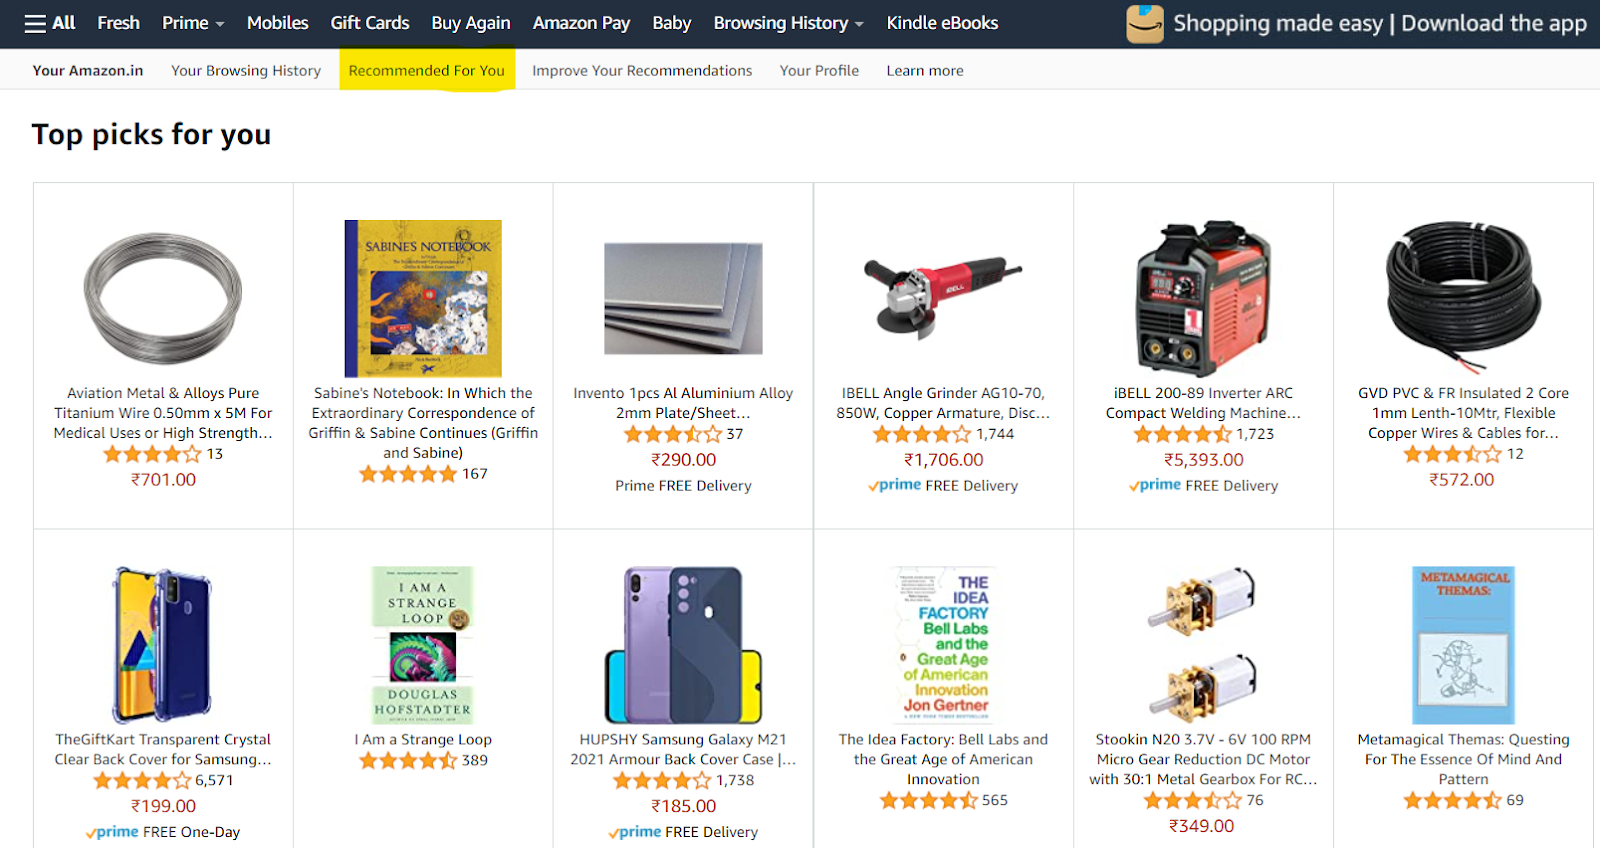
\includegraphics[width=1\linewidth]{images/amazonrecs.png}
    \caption{Recommendations on Amazon(\cite{Muralidharan_2023})}
    \label{fig:amazon}
\end{figure}
\begin{figure}
    \centering
    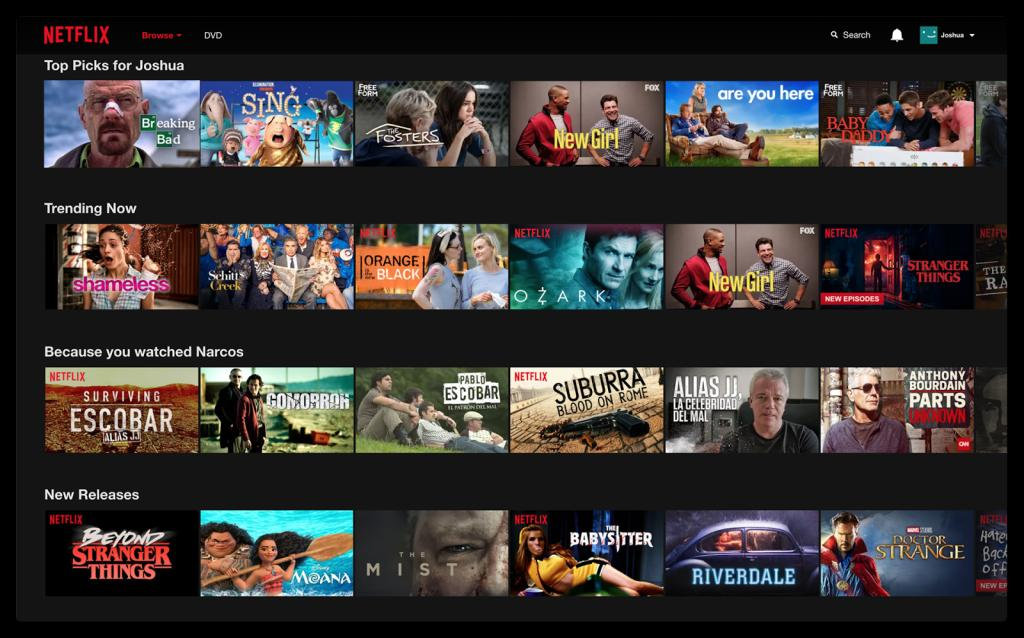
\includegraphics[width=1\linewidth]{images/netflixrecs.png}
    \caption{Recommendations on Netflix(\cite{Krysik_2021})}
    \label{fig:netflix}
\end{figure}
Recommender systems are found in different forms and serve a wide variety of purposes in many applications and services available to the consumer today, e.g. Netflix, Amazon, Spotify, YouTube (\cite{NflixResearch}, \cite{Hardesty_2024}, \cite{SpotifyResearch}, \cite{Goodrow_2021}), as seen in Figures \ref{fig:amazon} and \ref{fig:netflix}. They are products that seek to learn about and understand users in order to deliver `personalised' information to achieve `customer satisfaction'(\cite{Karakayali_Kostem_Galip_2017}). All recommender systems in their basic forms record some kind of user activity and behaviour(\cite{Paul_Kundu_2019}) to deliver recommendations on films, music, products, and many more(\cite{Yedidi_2023}). Recommender systems are usually split into three different categories: content-based recommender systems, collaborative recommender systems and hybrid recommender systems(\cite{Roy_Dutta_2022}), with each category being analysed in this section. Furthermore, this section contains analysis of the challenges faced in the current state of recommender systems. 
\subsection{Content-based Recommender Systems}
In content-based recommender systems, all items are classified based on their description or features(\cite{Roy_Dutta_2022}). For example, in a content-based recommender system for movies, features can be movie genres, directors, actors, year of release etc. Features are assigned to items automatically or manually, and must be represented in a way that items can be compared meaningfully, as items are recommended based on the comparison between available items and items in the user's profile(\cite{Paul_Kundu_2019}). The developed algorithm for the system must be able to thoroughly analyse a user's profile in order to make recommendations(\cite{Paul_Kundu_2019}). This approach can recommend items based on a little amount of data, however its correctness is reliant upon the model of features assigned to items(\cite{Paul_Kundu_2019}). Other advantages of content-based recommender systems are that they can adapt to a user's preferences changing over time, and that data of other users is not required to give recommendations, increasing data privacy and security(\cite{Roy_Dutta_2022}). Figure \ref{fig:content-based} represents the workflow of a Content-based Recommender System.
\begin{figure}
    \centering
    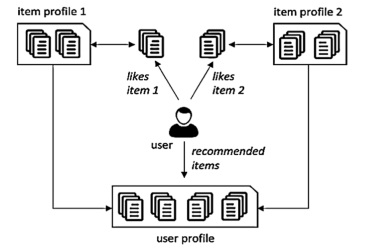
\includegraphics[width=0.55\linewidth]{images/Content-based-RS.png}
    \caption{Content-based Recommender System(\cite{Roy_Dutta_2022})}
    \label{fig:content-based}
\end{figure}
\subsection{Collaboration-based Recommender Systems}
Collaboration-based(or Collaborative filtering-based) recommender systems collect the preferences of many users and give recommendations based on the taste of others that have similar preferences as the user(\cite{Paul_Kundu_2019}, \cite{Roy_Dutta_2022}). This approach relies on the algorithm that determines the user's `neighbourhood', i.e. the set of users with similar tastes(\cite{Roy_Dutta_2022}). Rating systems in this approach are split into explicit: a user-defined rating scale e.g. stars, likes; and implicit: based on user activity and behaviour(\cite{Paul_Kundu_2019}). This approach suffers from a few drawbacks. Firstly, the cold-start problem entails that recommendations at early stages are poor as there is an insufficient amount of data to extract inferences from(\cite{Paul_Kundu_2019}, \cite{Roy_Dutta_2022}). The cold-start problem occurs when a new user or a new item is registered(\cite{Schedl_Zamani_Chen_Deldjoo_Elahi_2018}). Further analysis of the cold-start problem takes place further on. Figure \ref{fig:collab-based} represents the workflow of a Collaboration-based Recommender System.
\begin{figure}
    \centering
    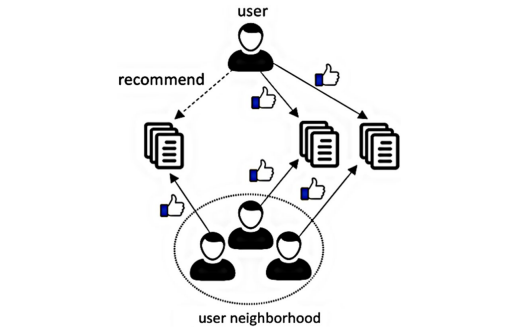
\includegraphics[width=0.55\linewidth]{images/Collab-based-RS.png}
    \caption{Collaboration-based Recommender System(\cite{Roy_Dutta_2022})}
    \label{fig:collab-based}
\end{figure}
\subsection{Hybrid Recommender Systems}
To address limitations faced by individual recommender system techniques, hybrid recommender systems are developed: a combination of two or more recommendation techniques(\cite{Roy_Dutta_2022}). In addition to different techniques working simultaneously resulting in the systems mitigating each other's drawbacks, these approaches are usually significantly more efficient and effective in delivering high-quality recommendations to the user(\cite{Paul_Kundu_2019}, \cite{Roy_Dutta_2022}). For example, hybrid algorithms may incorporate content-based filtering in a collaboration-based system or vice-versa(\cite{Roy_Dutta_2022}). Some approaches to hybridization(which are beyond the scope of this project but mentioned for posterity) include meta-level, feature-combination, and cascade hybridization(\cite{Roy_Dutta_2022}). Many industry leaders use hybrid recommender systems for their algorithms: For example, Amazon's ``item-to-item collaborative filtering" and YouTube's combination of collaborative filtering and using video metrics like Watchtime and Likes(\cite{Hardesty_2024}, \cite{Goodrow_2021}).
\subsection{Challenges faced by Recommender Systems}
\subsubsection{Cold start problem}
The Cold-start problem(as mentioned above) is the issue where the recommendation system cannot draw inferences from existing data, usually because the amount of data is insufficient for the algorithm, and usually occurs when the user or the item is new in the system(\cite{Roy_Dutta_2022}, \cite{Schedl_Zamani_Chen_Deldjoo_Elahi_2018}). As a result, new (or cold) users who have not provided a sufficient amount of ratings are not delivered high-quality recommendations(\cite{Roy_Dutta_2022}). Solutions to this issue include asking users to enter their preferences, asking users to rate items on sign-up, and collecting user data like location or age and presenting items similar users(according to the data collected) have rated positively(\cite{Paul_Kundu_2019}, \cite{Roy_Dutta_2022}). Figure \ref{fig:coldstart} accurately illustrates the cold start problem, with systematic bootstrapping referring to the initialisation of the system(\cite{Lendave_2021}).
\begin{figure}
    \centering
    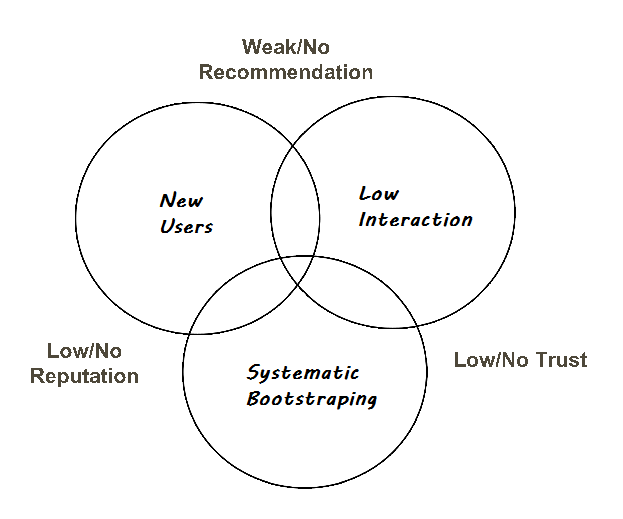
\includegraphics[width=0.75\linewidth]{images/coldstart.png}
    \caption{The cold start problem(\cite{Lendave_2021})}
    \label{fig:coldstart}
\end{figure}
\subsubsection{Scalability}
Scalability issues arise in recommender systems as these systems deal with massive amounts of data, with new items constantly being added at rapid rates(\cite{Roy_Dutta_2022}). This problem can be seen as the opposite of the cold start problem, as the systems might not be able to properly handle the storage and server load of the large volumes of new items and users. Solutions to mitigate scalability issues in recommender issues are reducing dimensionality, and using clustering to group users and data into clusters instead of operating over the entire database for every user(\cite{Roy_Dutta_2022}).
\subsubsection{Other issues}
Other issues in recommender systems include shilling attacks, latency issues, the grey sheep problem, and more(\cite{Roy_Dutta_2022}). Shilling attacks describe situations where bad actors give multiple items intentionally dishonest ratings to either increase or decrease an item's prevalence in a system(\cite{Roy_Dutta_2022}). This results in the accuracy and reliability of a recommender system decreasing, with a solution to this being systems detecting these users, deleting their ratings, and banning them from the system(\cite{Roy_Dutta_2022}). Latency issues occur in collaboration-based recommender systems when the rapid addition of new items results in those items not being recommended as the system has not reviewed them yet(\cite{Roy_Dutta_2022}). Finally, the grey sheep problem is another collaboration-based recommender system-specific issue and arises when a user's preferences are unique to the degree where they cannot be placed into any user neighbourhood(\cite{Roy_Dutta_2022}). Consequently, the system fails to recommend high-quality recommendations to the user(\cite{Roy_Dutta_2022}).
\section{Music Recommender Systems}
\begin{figure}
    \centering
    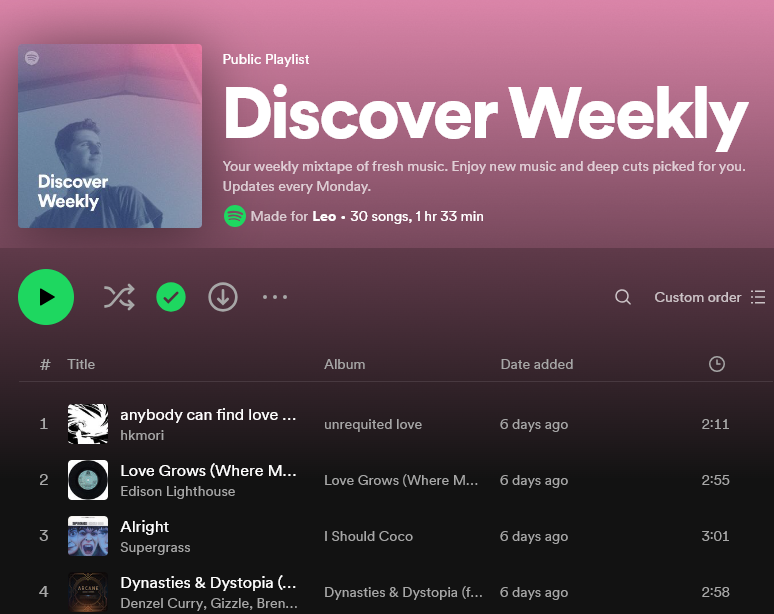
\includegraphics[width=0.75\linewidth]{images/discoverweekly.png}
    \caption{Spotify's Discover Weekly playlist with the description: ``Your weekly mixtape of fresh music. Enjoy new music and deep cuts just for you. Updates every Monday"}
    \label{fig:discover}
\end{figure}
\begin{figure}
    \centering
    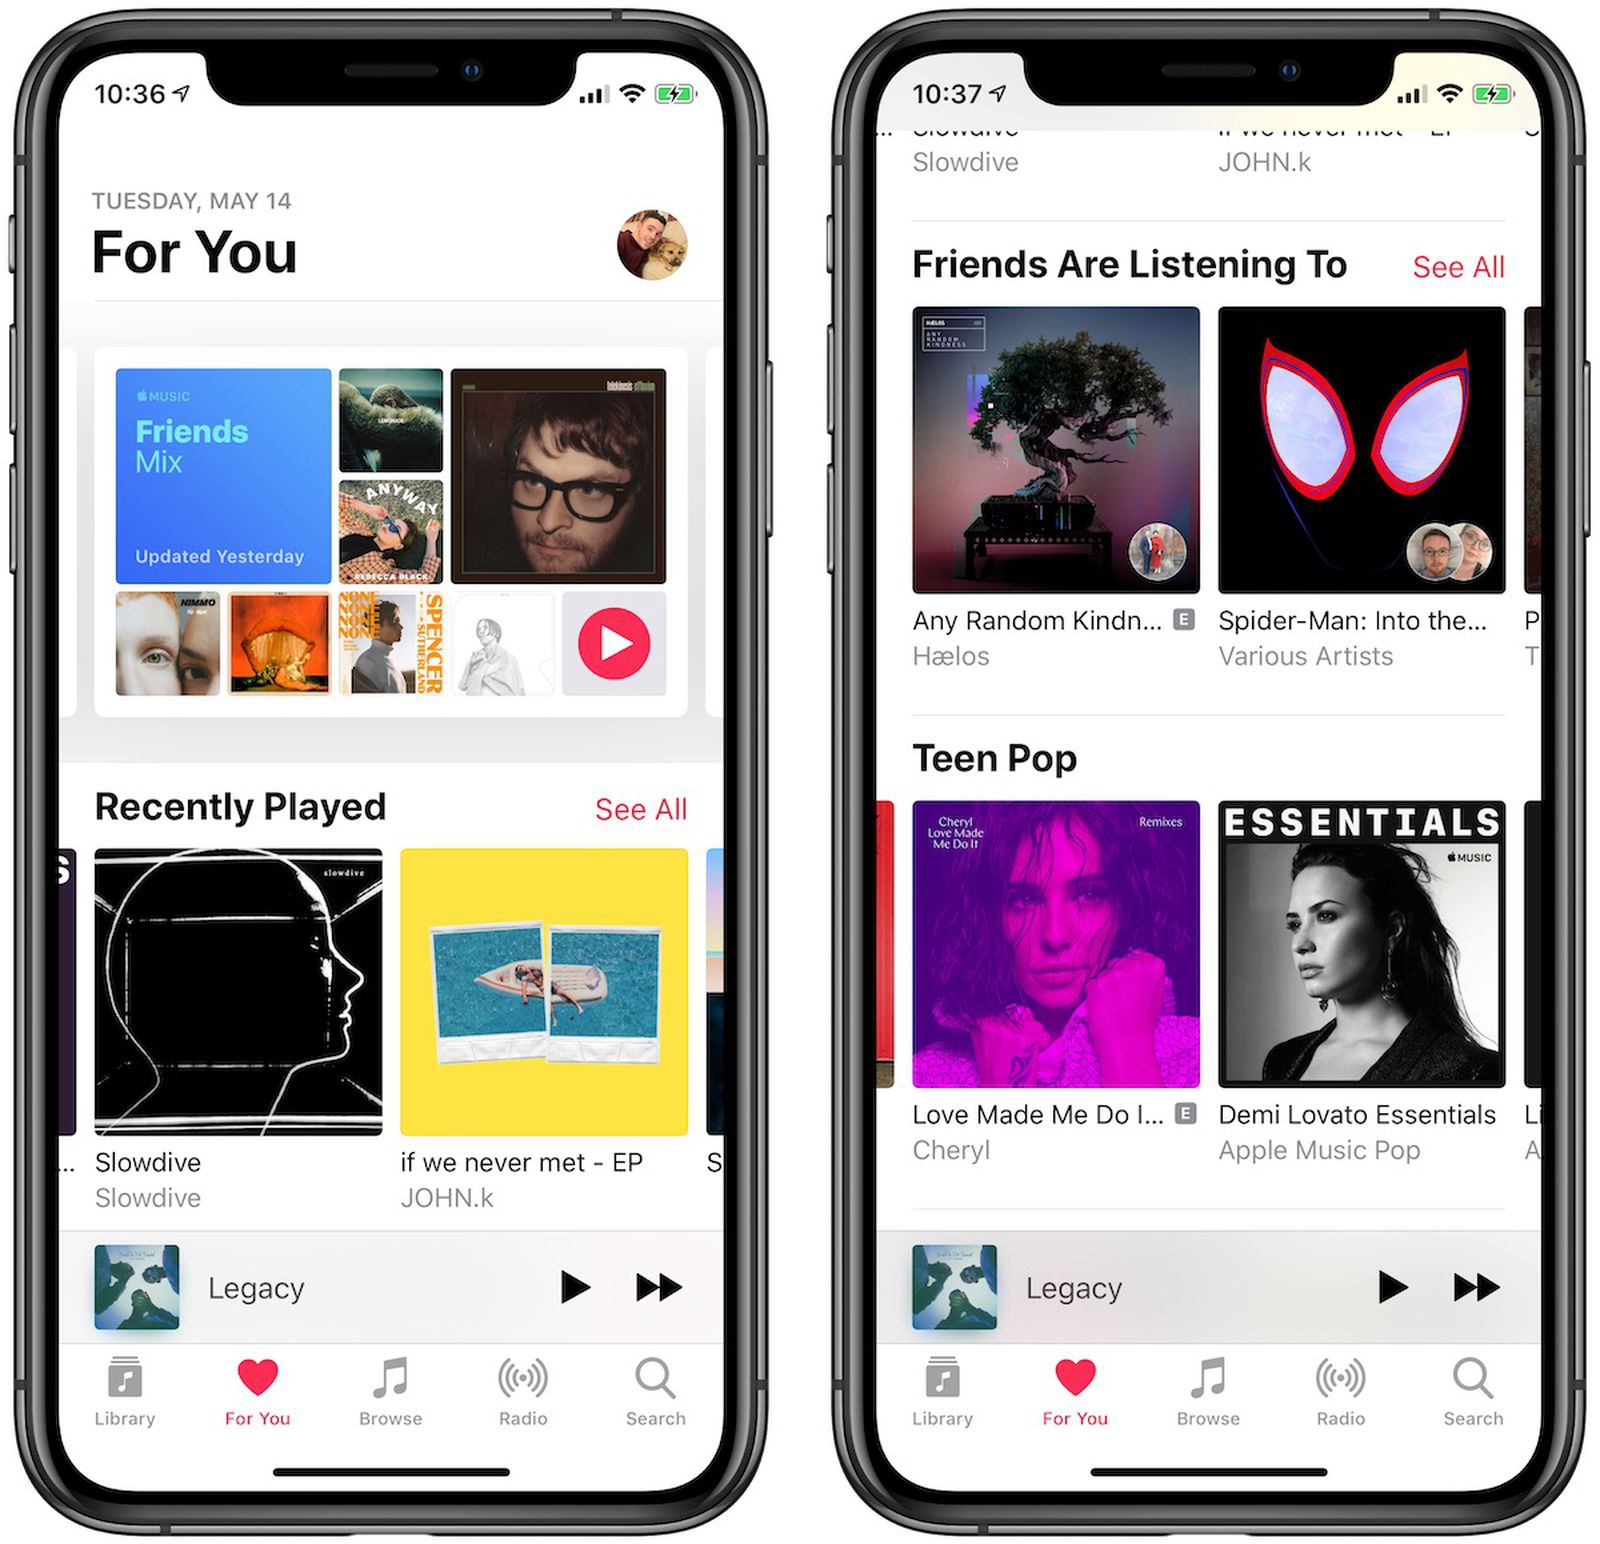
\includegraphics[width=0.5\linewidth]{images/apple-music-for-you-514.jpg}
    \caption{Apple Music's For You tab(\cite{Broussard_2019})}
    \label{fig:apple}
\end{figure}
Music Recommender Systems are recommender systems specifically tailored to recommending songs, music artists, or albums to users of their platform. They rely on user listening activity and behaviour, reducing the human effort it takes to discover new music by automatically recommending music based on various factors(\cite{Paul_Kundu_2019}). Major music streaming platforms like Spotify and Apple Music deploy recommender systems(as seen in Figures \ref{fig:discover} and \ref{fig:apple}) to allow users to ``explore their taste" by ``building highly effective, personalized and interactive models that exploit contextual information and historical user interactions"(\cite{SpotifyResearch}). This section will take the aspects and approaches to recommender systems mentioned in the previous section and analyse their applications and respective counterparts in music. In addition, this section contains analysis of challenges mentioned previously that music recommender systems also face, as well as challenges unique to music recommender systems. Moreover, this section explores the effect of music recommender systems on music taste, as people often rely on these systems to discover music(\cite{Karakayali_Kostem_Galip_2017}). This section is crucial to this project, as the main goal was to develop a tool that can recommend music to users based on their preferences.
\subsection{Content-based Music Recommender Systems}
As mentioned in the previous section, content-based recommender systems, when applied to music, recommend items(in this case songs) based on how similar songs are to a user's taste profile(\cite{Paul_Kundu_2019}). The model the system uses to assign terms to songs is crucial to the quality of recommendations delivered (\cite{Paul_Kundu_2019}). In the case of this project and many other systems, the terms(or tags) assigned to songs are based on genres/sub-genres of music, although other systems could analyse the acoustic features of a song(loudness, tempo, rhythm, etc.) to calculate recommendations(\cite{Paul_Kundu_2019}). Once terms are assigned, the most common methods systems employ to compute similarity are K-means clustering and expectation-maximization with Monte Carlo sampling(\cite{Paul_Kundu_2019}). While the cold start problem certainly exists in music recommender systems, content-based music recommender systems can overcome it, as they can recommend songs with a very small amount of data gathered(\cite{Paul_Kundu_2019}).
\subsection{Collaboration-based Music Recommender Systems}
Collaboration-based Music Recommender Systems generate recommendations to users by collecting the preferences and music tastes of many users(\cite{Paul_Kundu_2019}). In addition to recording user listening activity and behaviour(implicit ratings), these systems could utilise explicit user ratings, although that requires consistency in user rating habits(\cite{Paul_Kundu_2019}). As mentioned in the previous section, this approach can suffer from the cold start problem, resulting in poor initial recommendations(\cite{Paul_Kundu_2019}). Furthermore, if the user is aware that their ratings are needed to generate recommendations, they are less likely to rate songs the more effort it takes to generate recommendations(\cite{Paul_Kundu_2019}). K-nearest neighbours algorithms are used to split users into similar taste groups(\cite{Paul_Kundu_2019}).
\subsection{Hybrid Music Recommender Systems}
Hybrid Music Recommender Systems are far superior to single model systems when it comes to delivering high-quality music recommendations(\cite{Paul_Kundu_2019}). The combination of multiple systems results in the drawbacks of any single system included in the model being dulled(\cite{Paul_Kundu_2019}). For example, a Hybrid Music Recommender System could overcome the cold start problem mainly faced by collaboration-based systems by asking users what genres they prefer on sign-up(content-based) to initially recommend songs as the user's taste profile is slowly being built. In order to have a music recommendation system that is competitive in industry, that system would have to be hybrid. For example, Spotify uses a hybrid recommender system to deliver recommendations(\cite{Mohan_2023}). While the Song Recommendation Tool developed for this project is not at all at the same level of complexity as an industry-leading music recommender system, it is also a Hybrid Music Recommender System.
\subsection{Other approaches to Music Recommender Systems}
Some other methods that have been developed in the field of music recommendation systems and algorithms are: Emotion-based Filtering, Context-based Models, Cross-domain recommendations, and more in-depth analysis of a user's listening history(\cite{Paul_Kundu_2019})(\cite{Schedl_Zamani_Chen_Deldjoo_Elahi_2018}). 
\subsubsection{Emotion-based Filtering}Firstly, systems that use Emotion-based Filtering, as the name suggests, utilise a song's acoustic features to determine the emotions that the song may trigger, and recommend songs that trigger the same emotion(\cite{Paul_Kundu_2019}). These systems are based on the great research effort about how a user's mood affects their selection of music, and vice-versa(\cite{Paul_Kundu_2019}). Drawbacks of this approach are that it requires massive volumes of data to be collected to train the model and that there is ambiguity in the dataset as different people process emotions differently(\cite{Paul_Kundu_2019}).
\subsubsection{Context-based Models} Context-based(or situation-aware) models for recommending music utilise multiple factors in the user's environment to deliver high-quality recommendations. For example, these systems could recommend items based on their perception on social media and their popularity(how streaming platforms use charts)(\cite{Paul_Kundu_2019}). These kinds of recommendations could become even more personalised by recommending songs popular in the user's region(\cite{Paul_Kundu_2019}). Furthermore, Context-based Models can further utilise user location by taking into consideration the building they are in(library, gym, office, etc.)(\cite{Schedl_Zamani_Chen_Deldjoo_Elahi_2018}). Other factors these systems could consider are the time of day, social context(alone or with company), activity, weather, and day of the week(\cite{Schedl_Zamani_Chen_Deldjoo_Elahi_2018}). Research shows that these situational signals are strong indicators in search engine performance, and therefore could perform similarly for music recommendation(\cite{Schedl_Zamani_Chen_Deldjoo_Elahi_2018}).
\subsubsection{Cross-domain recommendations} Cross-domain recommender systems use data from other media domains to understand the user's taste and make recommendations(\cite{Schedl_Zamani_Chen_Deldjoo_Elahi_2018}). For example, a user's preferences in movies or books could be collected, processed, and music recommendations of a similar style could be derived and delivered.
\subsubsection{Further analysis of user listening history} While listening history is the base of music recommender systems, this dataset can be analysed and processed even further to derive more information about user habits. Breaking down this data into separate sessions of listening to music can provide insights into what users listen to in succession, their short-term preferences, and their long-term preferences(\cite{Paul_Kundu_2019}).
\subsection{Challenges faced by Music Recommender Systems}
Similarly to Recommender Systems in general, Music Recommender Systems face many of the same challenges. However, some of the challenges mentioned in this section are unique to Music Recommender Systems. Once again, this section will contain analysis of the cold-start problem(specifically for Music Recommendation). Furthermore, included in this section are explorations on the challenge of Automatic playlist continuation and issues with evaluating music recommender systems.
\subsubsection{Cold start problem} Following from the previous analysis of the cold start problem, there are aspects of this issue and approaches to overcome it unique to music recommender systems. For example, by extracting the acoustic properties of new items, inferences can be made about them, as this feature representation can accurately predict a user's taste(\cite{Schedl_Zamani_Chen_Deldjoo_Elahi_2018}). Moreover, if semantic labels are available(genres, instruments, etc.), it is possible to build models that can map acoustic features to semantic labels, making the feature representation even stronger(\cite{Schedl_Zamani_Chen_Deldjoo_Elahi_2018}). However, the acoustic features found in each song can be highly subjective(\cite{Schedl_Zamani_Chen_Deldjoo_Elahi_2018}). Hybrid systems consisting of collaborative as well as content-based filtering are also able to tackle this issue, although these systems are often much more complex, computationally expensive, and ambiguous(\cite{Schedl_Zamani_Chen_Deldjoo_Elahi_2018}). Using cross-domain recommendations(as mentioned above) and integrating other information about users that is unrelated to music can improve the estimate of their preferences(\cite{Schedl_Zamani_Chen_Deldjoo_Elahi_2018}). Despite that though, there are insufficient datasets for cross-domain systems, with cross-domain systems also requiring users and items to overlap(\cite{Schedl_Zamani_Chen_Deldjoo_Elahi_2018}).
\subsubsection{Automatic Playlist Continuation} Automatic Playlist Continuation(APC) is concerned with recommending songs to add to a user's playlist, with the new songs matching the characteristics of the original playlist. As seen in Figure \ref{fig:apc}, this is a feature included in Spotify where at the end of a playlist the user has created, there are recommended songs to add to the playlist based on the playlist itself. While it is a significant task for APC to infer the purpose of a playlist, if done successfully it enables users to extend their listening sessions beyond a playlist of finite length and makes it less difficult for them to enhance and lengthen their playlists without having to broader their music familiarity(\cite{Schedl_Zamani_Chen_Deldjoo_Elahi_2018}). On the other hand, this aspect of music recommendation also faces the cold start problem in the sense that it is difficult to recommend songs for a playlist when the playlist has just been created or is of very limited length(\cite{Schedl_Zamani_Chen_Deldjoo_Elahi_2018}). Another issue faced here is that it is not well understood if the ordering of tracks in playlists matters to the user(\cite{Schedl_Zamani_Chen_Deldjoo_Elahi_2018}). Moreover, current APC systems do not understand the implicit psychological and sociological factors that have to do with the decisions involved in creating a ``good" playlist(\cite{Schedl_Zamani_Chen_Deldjoo_Elahi_2018}).
\subsubsection{Evaluating Music Recommender Systems} While user satisfaction might be the most important measure of how successful music recommender systems are, research on evaluating music recommender systems is focused on accuracy, related quantitative measures, and novel beyond-accuracy measures like utility, serendipity, and novelty(\cite{Schedl_Zamani_Chen_Deldjoo_Elahi_2018}). While beyond the scope of this project, some state-of-the-art quantitative performance measures include mean absolute error, mean average precision at top K recommendations, Normalized discount cumulative gain, Mean percentile rank, and many more(\cite{Schedl_Zamani_Chen_Deldjoo_Elahi_2018}). Following on from the previous section on APC, evaluating APC systems requires sequence-aware evaluation measures(\cite{Schedl_Zamani_Chen_Deldjoo_Elahi_2018}). However, the focus on using quantitative measures to evaluate the performance of music recommender systems means that the user's experience is ignored(\cite{Schedl_Zamani_Chen_Deldjoo_Elahi_2018}). Even with beyond-accuracy measures like novelty and serendipity, their actual values might differ significantly from their perceived values, which means that user satisfaction cannot be fully measured(\cite{Schedl_Zamani_Chen_Deldjoo_Elahi_2018}). Therefore, holistic evaluation frameworks should be used to capture a better understanding of the user experience and of the performance of a music recommender system(\cite{Schedl_Zamani_Chen_Deldjoo_Elahi_2018}).
\begin{figure}
    \centering
    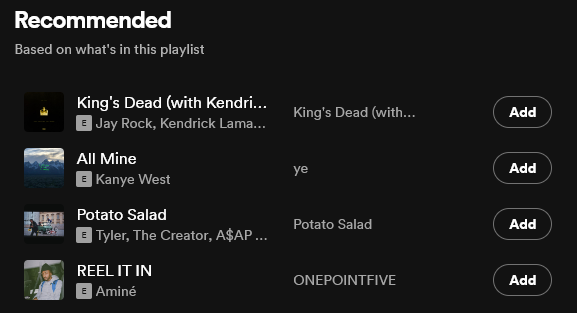
\includegraphics[width=0.85\linewidth]{images/APC.png}
    \caption{APC in Spotify}
    \label{fig:apc}
\end{figure}
\subsection{The effect of Music Recommender Systems on music taste}
For the avid music fan who is constantly seeking new music to listen to and enjoy, Music Recommender Systems can act more like `companions' than tools available to the user(\cite{Karakayali_Kostem_Galip_2017}). These systems can not only give the user control over their music taste with their algorithms, but they can also be hosts of a potential creative self-transformation for the user, as they are designed and developed to thoroughly understand the user in order to develop a highly personalised experience(\cite{Karakayali_Kostem_Galip_2017}). The effects a music recommender system can have on a user are co-constructed through the constant interactions between them(\cite{Karakayali_Kostem_Galip_2017}). Music Recommender Systems constantly hint at more and more music beyond the limits of the user's library to maximise engagement, the perpetual output of recommendations means that the diversification of the user's music taste is never completed, it is an endless pursuit(\cite{Karakayali_Kostem_Galip_2017}). There are potential bonds formed between the user and the Music Recommender System as information keeps flowing between them, with the user's music taste now the outcome of an activity(\cite{Karakayali_Kostem_Galip_2017}). Instead of only being a tool available to be used at the user's discretion, these systems become devices of `mediation' and `companionship', both going hand in hand(\cite{Karakayali_Kostem_Galip_2017}). While this might seem a bit extreme, an example of this ``companionship" with music recommender systems can be found in a large group of users of the social music discovery website last.fm, with these users sharing sentiments about how important these systems are to them(\cite{Schedl_Zamani_Chen_Deldjoo_Elahi_2018}).
\section{Bridging the Background with the Song Recommendation Tool}
Analysing recommender systems in general, the specifics of music recommender systems, the approaches to design these systems, the challenges they face, and the effect they have on their users was necessary, as the Song Recommendation Tool designed and developed for this project is through and through a Music Recommender System. Developing an understanding of content-based filtering, collaboration-based systems, and hybrid recommender systems is crucial in implementing an application that can deliver quality recommendations to its users. The challenges faced by recommender systems and more specifically music recommender systems need to be considered and accounted for during the process of creating this tool and for the tool to perform efficiently and effectively. While the Song Recommendation Tool might not be complex enough to have to deal with the issue of Automatic Playlist Continuation, the cold start problem and the issue of evaluating music recommender systems were significant aspects of properly implementing, testing, and evaluating the application. Realising the value recommendations can have to users, and how users view and use recommendations to expand and transform their music taste is inspiring in the pursuit to create a user-friendly and simple application that also motivates users to come back to it every time they're searching for new music to listen to. As seen in this chapter, music recommender systems(and recommender systems in general) are usually integrated into services that already offer the items they recommend, usually with the purpose of keeping constant user engagement with their service. Furthermore, the scale of these services alongside this integration of recommendations can make it unclear to the user which parts of their listening history are used to recommend which songs. The Song Recommendation Tool is a standalone tool, with the transparent goal of giving users music recommendations based on specific songs they enjoy, allowing them the additional freedom to manipulate their results to their liking with various parameters. The purpose of the Song Recommendation tool is to do away with the intensity of modern music recommender systems and to offer users a simple, straightforward, and transparent process of music recommendation.

%==================================================================================================================================
\chapter{Analysis/Requirements}
The description for this project provided by the project supervisor Chris McCaig outlined the following requirements: ``This project seeks to offer suggestions for songs a user may enjoy based on their ratings of other songs. Using a freely available dataset of song data (e.g. the Million Song Dataset) you will develop a song recommendation tool. This should allow a user to suggest a number of songs (say 5) with their own ratings of those songs. The tool would then recommend 1 song (or more than 1) that it predicts they will like. The tool should have a GUI interface for ease of use.". While this is a broad description of an application that can recommend music to users based on their preferences, it was a good starting point to begin the process of understanding the background and scope of the application. The next step was to do some research on how recommender systems work and to become familiar with them by working on a practical example of a recommender system for movies using data from IMDb. After finishing that, it was time to shift the focus onto the project itself. Now that a basic understanding of the technical foundations of recommender systems was acquired, the first decision to make was if the Song Recommendation Tool would utilise Content-based Filtering, Collaboration-based Filtering, or both for a hybrid approach. Once that was settled, the full list of requirements was devised. The requirements are outlined in this chapter and are split into functional and non-functional requirements. Both categories have sub-categories according to the MoSCoW framework.
\section{Functional Requirements}
Functional Requirements are requirements that describe actions the Song Recommendation Tool itself can process and complete. These requirements comprise the bulk of the implementation.
\subsection{Must Have}
\begin{itemize}
    \item Song Input: The user must be able to input songs and rate them.
    \item Recommendation Output: The program must output one or more recommendations based on the songs the user inputs.
    \item Recommendation Algorithm: The program must utilise a content-based filtering algorithm to determine recommendations for the user based on their preferences.
    \item Song Data: The program must contact some music API or keep a database of songs to operate on.
\end{itemize}
\subsection{Should Have}
\begin{itemize}
    \item Recommendation Algorithm: The program should utilise a combination of content-based and collaboration-based filtering to form a more complex and superior hybrid recommender system.
    \item Parameters: Other than songs, the user should be able to adjust various parameters to influence recommendations they get. For example, they should be able to set the number of recommendations they would like.
    \item Spotify Playlist Creation: The user should be able to create a Spotify Playlist with the recommendations the application gives them, through the application.
    \item Modify Input: The user should be able to remove songs they have input, and reset their input completely.
\end{itemize}
\subsection{Could Have}
\begin{itemize}
    \item Spotify User Listening History: Utilise 
 and display the user's Spotify listening history to avoid recommending songs the user knows and to give the user ideas of songs to input.
    \item Song Previews: Allow the user to listen to previews of recommended songs.
    \item Advanced Song Input: Show a list of possible songs the user could be trying to input while they are typing and allow them to click and add the correct option.
\end{itemize}
\section{Non-functional Requirements}
Non-functional requirements are other necessary additions to the application that are concerned with the application itself.
\subsection{Must Have}
\begin{itemize}
    \item Graphical User Interface: The Song Recommendation Tool must have a GUI in order for the user to be able to interact with the application.
    \item Local Deployment: The Song Recommendation Tool must be capable of being deployed locally on computer hardware that has the code-base.
    \item Performance: The Song Recommendation Tool must deliver relevant recommendations to users based on their preferences.
    \item Efficiency: The Song Recommendation Tool must deliver the recommendations in a reasonable time after the user is done with their input.
    \item Reliability: The Song Recommendsation Tool should not stop working unexpectedly and should report helpful error messages to users.
\end{itemize}
\subsection{Should Have}
\begin{itemize}
    \item Graphical User Interface: The GUI should be as simple and easy to use as possible to minimise user difficulty and confusion and to prioritise the aspect of the recommendations themselves.
    \item Guidance: The application should provide guidance to the user on how to use it and how to potentially utilise each parameter to influence their recommendations.
\end{itemize}
\subsection{Could Have}
\begin{itemize}
    \item Online deployment: Make the Song Recommendation Tool widely available by hosting it on an online platform.
    
\end{itemize}
%==================================================================================================================================
\chapter{Design}
The vision for the Song Recommendation Tool was clear at a very early stage. Designing the GUI happened with the following goal: Make the user interface as simple and user-friendly as possible, in combination with easy-to-understand instructions to make the user even more confident. Most of the hours spent on this project were attributed to working on the back-end, where songs were processed, the user's taste profile was created, and recommendations were derived. This chapter is a high-level overview of the solution that is the Song Recommendation Tool.
\section{Front-End}
The Front-end of the application is concerned with presenting all the possible actions that the user can select to complete. These actions need to be presented in a visually appealing way, prevents confusion, and motivates the user to engage with them. To reinforce this idea, a significant decision that was made very early in the development process was to house everything the application could provide on a single page. When considering the must-have features included in the Song Recommendation Tool, there was no need for pages to sign up/log-in or any account-creating aspects. While still having a sleek and modern look, the level of simplicity present in the Song Recommendation Tool aims to remind users of an older internet where corporations and services did not fervently seek to collect their personal information in exchange for a product. These companies make it their main goal to keep users constantly engaged in their products so they can monetize them in various ways. On the other hand, the ideal workflow for the Front-end of the Song Recommendation Tool can be described as(and can be seen in Figure \ref{fig:frontendworkflow}): Load up the page, input songs you want recommendations from, adjust some parameters to influence the recommendations based on your preferences, get the recommendations, optionally create a Spotify playlist populated with the recommendations, listen to the music, come back to the page if you would like to.
\begin{figure}
    \centering
    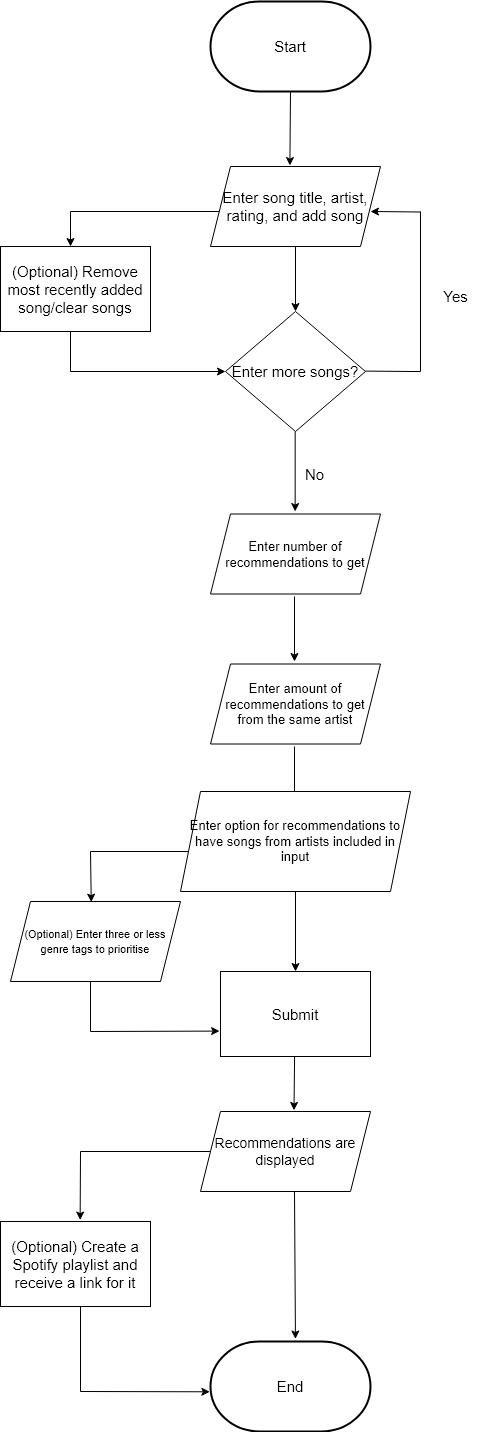
\includegraphics[width=0.6\linewidth]{images/UserWorkflow.drawio.png}
    \caption{Song Recommendation Tool Front-end workflow}
    \label{fig:frontendworkflow}
\end{figure}
There is no ulterior motive, the main goal is to provide users with music they would possibly like, hoping that inspires them to come back when they would like more recommendations. Wireframes were created before any of the styling of the website took place to create a general aesthetic idea of what the application could look like. One of these wireframes can be seen in Figure \ref{fig:wireframe}. The actual aesthetic design of the application is largely similar to the wireframes when it comes to the positioning of every component, with the current design sporting a different colour scheme. The current design of the Song Recommendation Tool can be seen in Figure \ref{fig:design}. As seen in Figure \ref{fig:design}, the application consists of a title, instructions for how to use the Song Recommendation Tool, input fields for song, artist name, and user rating as well as a button to submit the combination of those inputs, components displaying the songs the user has entered so far, buttons to remove the most recently added song and to clear all added songs, parameter input fields for number of recommendations they user would like, number of recommendations from the same artist, and a checkbox for users to enter whether they would like recommendations from artists they have input. Furthermore, there is a section where the user can view some popular genre tags, potentially enter any genre tags they would like to have prioritised in their taste profile, and finally, the submit button. While these parts are not visible in Figure \ref{fig:design}, after the submit button is clicked and processing is complete, recommendations are displayed in a continuous string of text, along with the user's taste profile, and a button to create a Spotify playlist. If that button is pressed, the user is redirected to a window where they need to authorize the use of their Spotify account to create the playlist(on Spotify's end), and if they consent, they are again redirected to a new instance of the Song Recommendation Tool where the link to their playlist is placed at the bottom of the page. The application also displays helpful error messages in situations where a user's input was incorrect or unable to be handled properly(more on that in the Implementation chapter). Overall, the design philosophy for the Front-end is to present the entire functionality of the application in one easily accessible and understood place, providing relevant features to the user, while simultaneously having a visually appealing look. 
\begin{figure}
    \centering
    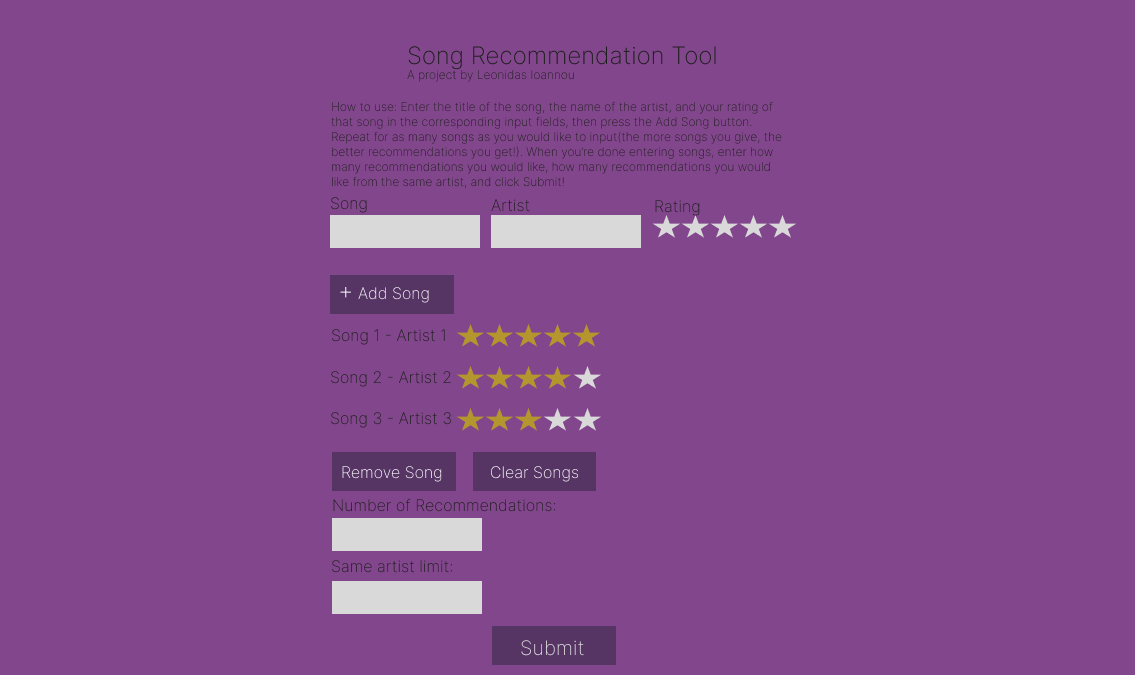
\includegraphics[width=1.0\linewidth]{images/Songs Added.png}
    \caption{Wireframe for the design}
    \label{fig:wireframe}
\end{figure}
\begin{figure}
    \centering
    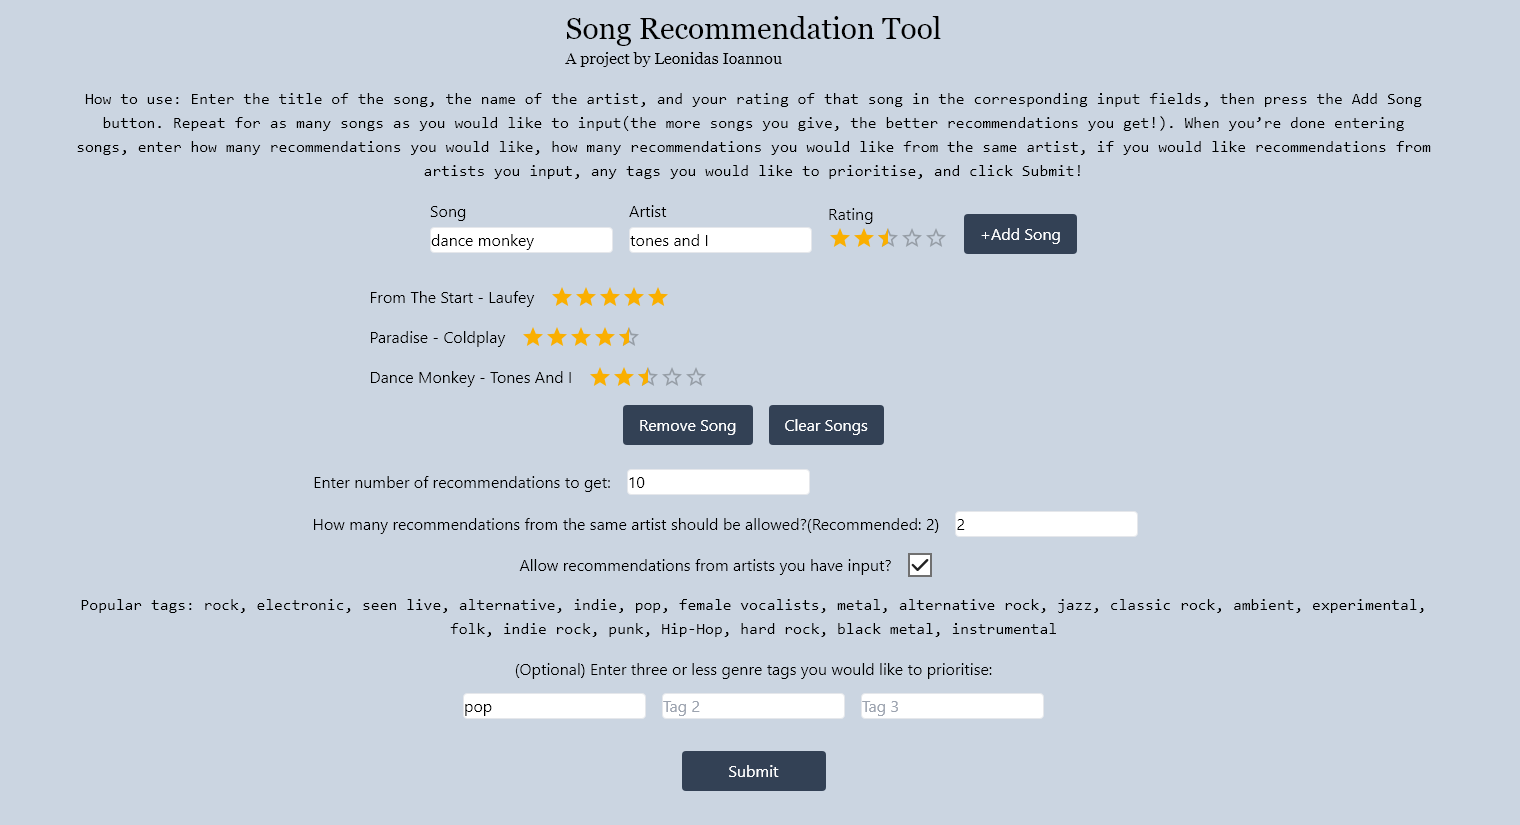
\includegraphics[width=1.0\linewidth]{images/actual_design.png}
    \caption{Current Design of the Song Recommendation Tool Front-end}
    \label{fig:design}
\end{figure}
\section{Back-End}
The Back-End of the Song Recommendation Tool is concerned with processing user input, creating the user's taste profile, gathering recommendations that are relevant to that taste profile, delivering them to the user, and overall implementing a hybrid Music Recommender System that consists of a mostly content-based system with collaboration-based elements. All these functionalities are stored in different interconnected functions in the Back-end code-base. This section aims to explain what each function does without referencing specific elements of code, present the workflow of the Back-end, and outline its overall design philosophy. There is one function that handles the events when the user inputs a song or clicks the remove song or clear songs buttons. The function(its general workflow can be seen in Figure \ref{fig:receiveworkflow}) communicates with other functions to obtain the classification tags of the song, to update the user's profile accordingly, or to return an error message relevant to the faulty action that occurred.
\begin{figure}
    \centering
    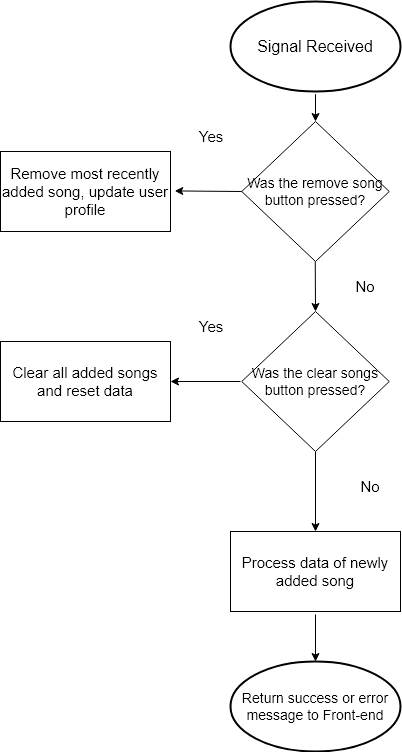
\includegraphics[width=0.5\linewidth]{images/receive_song.drawio.png}
    \caption{Function that handles add song/remove song/clear songs input}
    \label{fig:receiveworkflow}
\end{figure}
Another function handles the event when the submit button is clicked(its general workflow can be seen in Figure \ref{fig:submitworkflow}), therefore it processes all parameters the user inputs and communicates with other functions to derive recommendations, prepare Spotify playlist creation, and organise the recommendations before they are sent back to the Front-end.
\begin{figure}
    \centering
    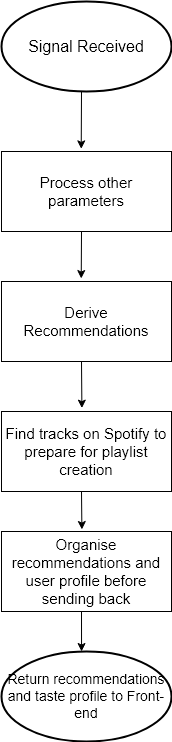
\includegraphics[width=0.25\linewidth]{images/Submit.drawio.png}
    \caption{Function that handles submit button click}
    \label{fig:submitworkflow}
\end{figure}
The next couple of functions deal with the Create Spotify playlist feature to gather the recommendations from Spotify, redirect the user to authorize their account through Spotify, create and populate the playlist with the already gathered songs, and send the link to the playlist to the Front-end. The function after that resets almost all data stored in the Back-end, which is necessary when the user clicks the Clear Songs button or for after the recommendations are sent to the Front-end, to prepare for the user's next set of inputs. The next four functions communicate with the source of song information the application uses to gather necessary information about songs and genre tags and to ensure that there is no faulty data obtained. The subsequent function is responsible for updating the user's profile once a new track comes in, with the last two remaining functions dealing with obtaining potential tracks to be recommended and determining which tracks are the best to recommend. While the workflow of the Back-end is much more complex than the workflow of the Front-end, the functions present in the Back-end have clear purposes and are distinct in what they do and how they accomplish it. These functions must operate properly in order to communicate with each other, as well as to communicate with the Front-end and with the external sources of information used for the Song Recommendation Tool.
\section{Design Summary}
Overall, the design of the Song Recommendation Tools fluctuates in complexity between the Front-end and the Back-end. The design of the Front-end is centered on being user-friendly and simple, with the features presented being easy to understand and use. On the other hand, the Back-end is populated with various interconnected functions, with each one serving a different purpose in implementing all the features the Song Recommendation Tool provides. Finally, the Song Recommendation Tool is designed in a way that enables efficient and effective communication between Front-end and Back-end, with more details about this given in the Implementation chapter.
%==================================================================================================================================
\chapter{Implementation}
This chapter aims to analyze the technical implementation and achievements of all aspects of the Song Recommendation Tool. While the chapter of Design outlined the high-level details and workflows throughout the application, this chapter references various specific pieces and sequences of code and what they accomplish for the application. Once again, it is relevant to split this analysis into Front-end and Back-end, as the Song Recommendation Tool as a project is a mix of Web Development and Data Science. Furthermore, another purpose of this chapter is to assess the technological stack and external data sources used to develop the Song Recommendation Tool. Finally, while the Song Recommendation Tool is successful in its purpose in the vast majority of situations, this chapter also addresses the few limitations faced by the application. 

\section{Technological Stack}
The Technological Stack used to implement the Song Recommendation Tool consists of two major elements: React for the Front-end implementation and Flask for the Back-end implementation. Both of these are Web Development frameworks that contain many useful features and are based on underlying languages: HTML and JavaScript for React, and Python for Flask. In addition, the Last.fm and Spotify APIs were used for it to be possible for various features to be implemented. The Last.fm API is the main source of data for the Song Recommendation Tool. This was a very early decision in the development process, for reasons that will be analysed in the Back-end section of this chapter. The Last.fm API is responsible for supplying the application with correct song titles and artist names, genre tags attached to each song, tracks that correspond to genre tags, and user listening data. The Spotify API is responsible for making the create a playlist feature possible throughout multiple steps, with these steps analysed in the Back-End section of this chapter. The application is currently hosted locally on the same Windows system it was developed on and is not reliant upon any external hosting services to be able to operate. Moreover, the Song Recommendation Tool is built for desktop use, with the Front-end styling done using Tailwind, which is a CSS framework that allows developers to efficiently style websites without the need for external CSS files. 
\section{Front-End}
Developed using React and styled using Tailwind, the Front-end is how the user can interact with the Song Recommendation Tool. React was chosen for the development of this project as there was existent familiarity with it, because it is a very efficient framework for Web Development, and because it can easily house and implement every feature the Song Recommendation Tool provides to its users. Another very useful feature in React is the ability to update different aspects of the application as the user interacts with it by using the State feature, which was used multiple times in the implementation(call a \texttt{useState} function for a specific variable when it is updated). All elements of code are styled using Tailwind to achieve the desired aesthetic appearance and position. In order to understand how the Front-end is structured from a code perspective, what follows is an analysis of all the different components present in the code, starting from the top of the page and moving toward the bottom. The topmost component of the Front-end is a section containing the title of the application, the subtitle, and a small paragraph of instructions on how to use the application which mostly describes the different buttons and input fields the user must or can utilise. Down from that, the next section contains the Add Song functionality. 
\subsection{Add Song}
Comprised of three input fields, the Add Song section is responsible for the input of song title, artist name, and user rating(songs are rated with stars from zero to five, with half stars also being available ratings e.g. 3 stars, 4.5 stars). Every input field is tracked with its own variable, with updates to those values happening with event handling and \texttt{useState} functions. Once the user has filled in the input fields, the next step is to click the Add Song. Once that occurs, the \texttt{addSongComponent} function is called, which calls the \texttt{sendAddData} function.
\subsubsection{\texttt{sendAddData}}
The first thing done in this function is updating the state of a variable to disable the Add Song, Remove Song, and Clear Songs buttons until the song processing is completed. Then, the function communicates with the Back-end, sending the track title, artist name, and rating. If the communication is successful, the function receives either a specific error message or the actual song data. These error messages are either for if the song was not found(and suggesting to the user that they check their spelling), for if the song has already been added, or if the added song has been found but does not have genre tags attached to it, and if the rating provided was invalid(either if the user did not enter a rating or if it is 0). Actual song data refers to the proper song title and artist name in the data source, with examples being if the user did not properly capitalise words in the song or artist names, or if they made slight spelling errors. If song data is received instead of an error message, a variable is updated to contain the data. The function also handles any errors that occur during communication, and finally re-enables the Add Song button once the processing is completed.
\subsubsection{Song Components}
Once the data for a song is received, a song component is added under the Add Song fields. Each component displays the proper song title, artist name, and user rating. These components are stored in an array(a list of elements), which is dynamically updated when a new song is added, a song is removed, or all songs are cleared. The way the components are displayed is through a specific React function which can display multiple array elements at once with one piece of code, which is a mapping between the list index of a component and its contents.
\subsection{Remove Song \& Clear Songs Buttons}
Below the song components are the Remove Song, and Clear Songs buttons. As their names suggest, these buttons allow the user to remove the most recently added song, and to clear all songs entered, respectively. How this works is as follows: the user clicks one of the buttons, and either the \texttt{sendRemoveData} or the \texttt{clearSongs} function is called.
\subsubsection{\texttt{sendRemoveData}}
\texttt{sendRemoveData} starts by disabling the Add Song, Remove Song, and Clear Songs buttons. After that, it communicates with the Back-end to inform it to remove the most recently added song. The response from the Back-end is either an error message saying that there are no songs to remove in the case where the user clicks the button when there are no songs present, or a successful response which then sets the song data variable to a signal that edits the song components to remove the most recently added song component. Finally, the Add Song, Remove Song, and Clear Songs buttons are re-enabled.
\subsubsection{\texttt{clearSongs}}
Firstly, \texttt{clearSongs} opens a pop-up window on the page asking the user to confirm that they indeed would like to clear all songs. If the user clicks "OK", then the function \texttt{sendClearData} is called. Then, \texttt{sendClearData}, similarly to \texttt{sendRemoveData}, disables the Add Song, Remove Song, and Clear Songs buttons. After that, the function sends a signal to the Back-end to clear all songs and reset the user's profile and other data. Once a response is received, if it is successful then the song data variable is set to a signal to clear and delete all song components. Once again, when all the processing is completed, the Add Song, Remove Song, and Clear Songs buttons are re-enabled. Figure \ref{fig:topcomps} shows the Add Song fields and button, the song components, and the Remove Song and Clear Songs buttons.
\begin{figure}
    \centering
    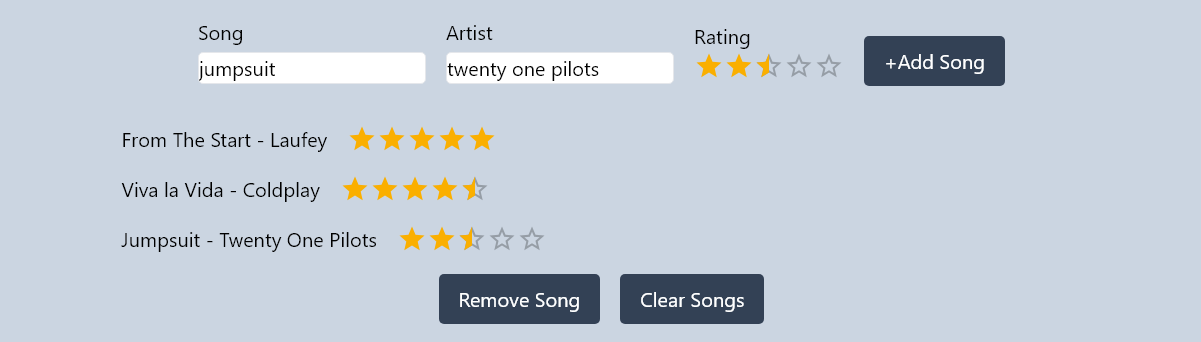
\includegraphics[width=1.0\linewidth]{images/topcomps.png}
    \caption{Add Song functionality, Song components, Remove Song button, Clear Songs button}
    \label{fig:topcomps}
\end{figure}
\subsection{Recommendation Parameters}
The Song Recommendation Tool provides multiple parameters that the user must or can enter to influence their recommendations. These parameters are as follows: Number of recommendations, Maximum number of recommendations from the same artist, Allow recommendations from artists in inputs, Tags to prioritise. The first three parameters are accompanied by their own input field next to text describing them(a checkbox for the third parameter), then there is a small piece of text giving the users examples of tags they could prioritise if they would like to, text describing the final parameter as well as an indicator that this parameter is optional, with three input fields for these tags below that. All these parameters are tracked with their own variables, and event handling functions, and updated using different \texttt{useState} functions. The parameter input fields can be seen in Figure \ref{fig:params}.
\begin{figure}
    \centering
    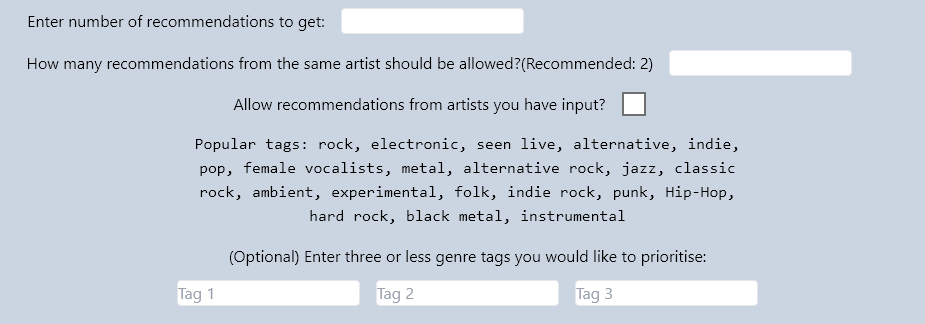
\includegraphics[width=1\linewidth]{images/params.png}
    \caption{Parameters that can influence recommendations}
    \label{fig:params}
\end{figure}
\subsection{Submit \& Recommendations}
Under the parameter inputs lies the Submit button. Once the Submit button is clicked, the function \texttt{submitSongs} is called.
\subsubsection{\texttt{submitSongs}}
Firstly, \texttt{submitSongs} disables the Submit button until processing is completed and recommendations are returned. Then, the function sends all the parameters mentioned in the previous sub-section to the Back-end. Once that happens, the function awaits the Back-end's response, which is usually the recommendations the user is waiting for. That response is then assigned to a variable that keeps the recommendations text. In the case where any of the parameters was for some reason invalid, the recommendations text is an error message indicating which parameter was an incorrect input. After that, the Create a Spotify playlist feature is enabled and the Submit button is re-enabled. Under the Submit button on the user interface, the recommendations are displayed as one continuous piece of text, with the user's taste profile below them. Finally, below that, the Create a Spotify Playlist button appears.
\subsection{Create a Spotify Playlist}
Once the Create a Spotify Playlist button appears, and the user clicks it, the process to Create a Spotify Playlist begins. First, the user is redirected to a Spotify Window to give the Song Recommendation Tool authorization to create a playlist on their profile. When the user grants authorization, Spotify provides the application with an authorization token. The application then disables the Create a Spotify Playlist button and sends that token to the Back-end so the Back-end can actually create the playlist. Simultaneously, once the user completes the authorization, they are redirected to a new window of the Song Recommendation Tool. Subsequently, the application awaits the Back-end's response, which is a link to the playlist. That link is then assigned to the playlist variable and the Create a Spotify Playlist button is re-enabled. The link is output on the new instance of the application along with any Spotify errors for any songs(these errors will be outlined in the Limitations section of this chapter). The Submit button, Recommendations and Taste profile, and Create a Spotify Playlist button can be seen in Figure \ref{fig:submit}.
\begin{figure}
    \centering
    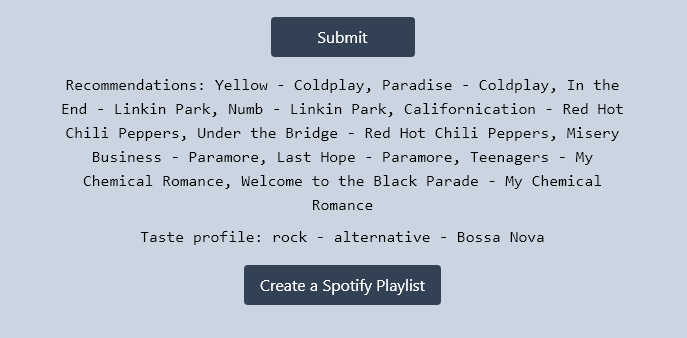
\includegraphics[width=1\linewidth]{images/Submit.png}
    \caption{The Submit button, Recommendations and Taste Profile, the Create a Spotify Playlist button}
    \label{fig:submit}
\end{figure}
\subsection{Front-End Summary}
Overall, the different features and functions provided by the Front-end are handled responsively and efficiently in React. Every function is distinct in the purpose it serves, and a proper communication framework is present, for the Front-End to be able to communicate with the Back-End. The multiple \texttt{useState} functions are crucial in ensuring that all variables are up to date with their latest values, depending on the user's actions. Finally, the styling options provided by Tailwind make the styling process easy and efficient, while still giving the Song Recommendation Tool a sleek look.
\section{Back-End}
Developed using the framework of Flask, and by extension Python, the Back-end is responsible for the implementation of the Data Science aspect of the Song Recommendation Tool. Flask is what makes the web development aspects possible, mainly the communications with the Front-End. This Python implementation deals with receiving various information and signals from the Front-end and other sources, gathers and processes data, derives results, and returns those results to the Front-end. Work on the Back-end was lengthy, was a lot less formulaic, and required a lot more computational thinking and problem-solving than developing the Front-end did. The success of the Song Recommendation Tool hinges upon the Back-end, as song recommendations are calculated in one of its many functions. By using a hybrid recommendation system, the Back-end aims to provide high-quality music recommendations to the users of the Song Recommendation Tool. Furthermore, the Back-end utilises two APIs(Application Programming Interfaces) to gather data and to provide more features: The Last.fm API and the Spotify API. The next sub-section contains an analysis of the Last.fm API and how the Song Recommendation Tool is reliant on it, with the Spotify API used exclusively for required methods to provide the Create a Spotify Playlist feature.
\subsection{Song and Genre Data: Last.fm}
Perhaps the most important decision to be made regarding the development of the Song Recommendation Tool was the choice of what music dataset/data source to operate upon to understand what the user likes and give them relevant recommendations. Some of the suggestions provided by the project supervisor were interesting(e.g. the Million Song Dataset) but they were rejected due to a very important reason. While they were complete datasets in terms of each item's classification, they were not at all recent, with some being at least 10 years old. For the Song Recommendation Tool to even be considered useful to a modern user, it would most definitely require its data to be as up-to-date as possible. For that reason, instead of using a dataset, the Song Recommendation Tool uses an API to gather data: The Last.fm API. This approach provides several benefits, as well as some drawbacks(drawbacks discussed and analysed in the Limitations section of this chapter). According to their website, Last.fm is a platform to ``track, find, and rediscover music"(\cite{Last.fm}). Their API is extremely useful when it comes to gathering information about songs and genre tags. Songs can have multiple tags attached to them and tags can be looked up to retrieve the most popular songs that are in their category. Other than this approach providing mostly up-to-date data to the Song Recommendation Tool, gathering data as needed from the API keeps the application lightweight, as there is no need to store massive volumes of song data. Furthermore, while the fact that the application uses the genre tags on each song to build the user's profile and derive recommendations, the tags on Last.fm are applied to songs by the large user base, with the order of tags on a song being determined by how many users believe a tag belongs to a song. This approach to item classification already sets up the foundation of a hybrid Music Recommender System, which is what the Song Recommendation Tool is. Using the Last.fm API requires an application authorization token, which was obtained by communicating with the company via e-mail. More information about the Last.fm API can be found at: \url{https://www.last.fm/api}
\subsection{Receiving Songs from the Front-End}
The first step to using the Song Recommendation Tool is to add a song to the system. As mentioned above, the song information is sent from the Front-end to the Back-end. In the Back-end, that information is received by the \texttt{receive\_song} function. This function also handles signals from the Remove Song button and the Clear Songs button. Firstly, it checks if the signal is to remove the most recent song and if so attempts to remove the song from the list of songs the user has input, and to modify the user's profile to not be affected by the song to be removed. If it is successful, a success message is returned to the Front-end, and if not, an error message saying that there were no songs to remove is returned. If the signal is to clear all songs, the function just calls the reset function, which resets all user data for this session of use. Now that those cases have been handled, the rest of the function deals with the case of when the user actually inputs a song. First, the information received(song title, artist name, rating) is split and assigned to a song data list. The first check is to make sure that the rating is valid; if not, an error is returned. Then, the \texttt{lastfm\_get} function is called, with the song title and artist name passed into it.
\subsubsection{\texttt{lastfm\_get}}
This function communicates with the Last.fm API to search for the track supplied by the user. If a track is found, the function communicates with the Last.fm API again, this time to obtain the top genre/sub-genre tags attached to the track. Subsequently, the track and artist names found on Last.fm, along with the tags are returned to \texttt{receive\_song}. If a track is not found, an error message indicating that is returned to \texttt{receive\_song}.
\subsubsection{Return to \texttt{receive\_song}}
If the response from \texttt{lastfm\_get} is the error message, the Front-end receives an error message that the song could not be found. If the track returned from \texttt{lastfm\_get} is already in the system, the Front-end receives an error message that the song has already been added. After those error checks, the function \texttt{gettags} is called, with the tags returned from \texttt{lastfm\_get} passed into it.
\subsubsection{\texttt{gettags}}
The goal of \texttt{gettags} is to build a list of the top three actual genre/sub-genre tags attached to a song. Only the top three are considered as tags are ranked depending on how many users think they are appropriate for that song. Therefore, three is a good amount to avoid retrieving less accurate tags for each song. The function also ensures that the genre/sub-genre tag to be added to the final list is not a false tag(some tags are just numbers or references to other applications). Once a list of three tags(the number of times each tag was added to a song is also stored alongside each tag) is assembled, it is returned to \texttt{receive\_song}. After the tags are returned and a part of the content-based filtering approach is fulfilled, the function \texttt{lastfm\_similar} is called to fulfill a collaboration-based filtering aspect of the Song Recommendation Tool.
\subsubsection{\texttt{lastfm\_similar}}
Communicating with the Last.fm API, \texttt{lastfm\_similar} retrieves five tracks that are similar to the track the user has input, with similarity being measured using user listening history exclusively. Once tracks are gathered, they are saved in a variable tracking these similar songs, with the frequency in which they have appeared being recorded. For example, if Song A is retrieved in \texttt{lastfm\_similar} during the processing of when the user inputs Song B, and when the user inputs Song C, the fact that Song A has appeared twice is recorded. This feature is used later when recommendations are being calculated.
\subsubsection{Return to \texttt{receive\_song}}
Back to \texttt{receive\_song}, the three tags recorded for the song are stored in a list which is in turn stored in a Python dictionary which tracks each song and its tags. The name of the artist that made the song is stored in a list that tracks the artists the user has input, and then the function \texttt{updateprofile} is called, with the song's tags and rating passed into it.
\subsubsection{\texttt{updateprofile}}
Inside \texttt{updateprofile}, the list of tags is iterated through to update the score of a tag, or to create a new entry for a tag. The structure of the user's profile is a Python dictionary, with keys being tags and values being each tag's numeric score. The value to be added to a tag is the number of times the tag was added to that song on Last.fm multiplied by the user's rating of that song. Hence, if that tag already exists in the user's profile, the new value is added to the value already there, and if the tag is new to the user's profile, then the new value is that tag's initial value. An example profile can be seen in Figure \ref{fig:prof}. The user's profile is always stored in descending order from the tag with the highest score to the tag with the lowest score and is sorted inside \texttt{updateprofile}. 
\begin{figure}
    \centering
    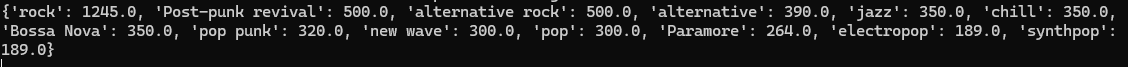
\includegraphics[width=1\linewidth]{images/profile.png}
    \caption{An example of a potential full user profile.}
    \label{fig:prof}
\end{figure}
\subsubsection{Final actions of \texttt{receive\_song}}
After the profile is updated, the last thing receive\_song does is check if the list of tags is empty. This can happen in cases where a song may not be well known enough for users to attach tags to it on Last.fm. If that is the case, an error message indicating this is returned to the Front-end. Otherwise, the proper track title and artist name obtained from Last.fm are returned to the Front-end, to be added to the song components.
\subsection{Submit}
The Back-end function that handles the Front-end signal when the user clicks the Submit button is \texttt{submit\_songs}. Once the signal is received, the function parses the different input parameters mentioned in the Front-end section(number of recommendations, tags to prioritise, etc.), and assigns each one to its own variable(tags to prioritise are stored in a list). Then, if the tags the user has chosen to prioritise are present in their profile, the scores of those tags are boosted. Now that the profile has been potentially modified, it is sorted in descending order again and passed into the \texttt{get\_data} function.
\subsubsection{\texttt{get\_data}}
The goal of \texttt{get\_data} is to gather songs and artists that correspond to the user's profile. To accomplish that, the process is split into two parts of communication with the Last.fm API. Firstly, the function iterates through the tags in the user's profile and retrieves the top songs corresponding to each tag. A maximum of 200 songs are obtained for every tag. Secondly, the profile is iterated through again, this time to retrieve the top artists corresponding to each tag. A maximum of 50 artists are obtained for each tag. Finally, this function returns two variables. A Python dictionary mapping a piece of text indicating song title and artist name with a list containing the song's artist and the tag the song corresponds to(if a song corresponds to multiple tags, and the artist has been obtained by the function, the tag attached to the song is the tag attached to the artist). In addition, the list of artists is also returned. 
\subsubsection{Return to \texttt{submit\_songs}}
Back to \texttt{submit\_songs}, the function performs some error handling. If the user's profile is empty, a relevant error message is returned to the Front-end. If the number of recommendations asked for is an invalid number(or not a number at all), an error message is returned. The parameter of number of recommendations from the same artist to be allowed is handled in the same way. Next, the function that finally derives the recommendations is called, \texttt{calcscores}.
\subsubsection{\texttt{calcscores}}
The parameters taken by \texttt{calcscores} are the user's profile, the two variables returned by \texttt{get\_data}, the number of recommendations to be derived, the number of recommendations from the same artist to be allowed, and the variable that indicates if recommendations from input artists should be allowed. Since the list of artists is naturally sorted from the way it was created(the first artist in the list is the most popular artist of the user's highest-scoring tag, the 150th artist is the 50th most popular artist of the user's third highest-scoring tag), the first 150 artists are given a score corresponding to their popularity and to which tag they belong to. The first 50 artists are given a score of \texttt{(50-popularity) * 3}, artists in positions 51-100 are given a score of \texttt{(100-popularity) * 2}, and artists in positions 101-150 are given a score of \texttt{150 - popularity}. All artist scores are stored in a dictionary where the keys are artist names and values are scores. After that, all tracks receive scores with the following algorithm, inside a loop that iterates through all tracks: 
\begin{enumerate}
    \item Initialise the score of every track to 1.
    \item If a song was made by an artist included in the list of artist scores, the track's score becomes the artist's score.
    \item If a song was made by an artist the user has input, boost the track's score by 150. This is useful in cases where the music is potentially obscure and not many tracks have been obtained.
    \item If the tag attached to the song is the user's highest scoring tag, triple the track's score.
    \item If the tag attached to the song is the user's second-highest, double the track's score.
    \item If the track is included in the list of Last.fm user listening history based similar tracks, its score is boosted by \texttt{100 * }(times it was mentioned as a similar track).
\end{enumerate}
Now that all tracks have a score, they are sorted in descending order by score. The next step is to gather a list of as many recommendations as the user wants, being careful not to include more recommendations from the same artist than the user has specified, and ignoring tracks from artists the user has input if the user has specified that they would not like that for their recommendations. The list assembled is the recommendations to be returned to the Front-end, but it is first returned to \texttt{submit\_songs}, which now prepares the Create a Spotify Playlist feature by passing the recommendations into \texttt{get\_spot\_ids}.
\subsubsection{\texttt{get\_spot\_ids}}
This function communicates with the Spotify API to retrieve the track IDs of the recommended tracks. It is important to mention that the Song Recommendation Tool was registered to use the Spotify API and various tokens were provided by Spotify to enable the use of the API by the application. The IDs mentioned are necessary to later populate the playlist with the songs. IDs are retrieved by searching for the track using the Spotify API's search method. For a reason that will be explained in the Limitations section of this chapter, various search cases exist to try and find a track by using the Spotify API. These cases are as follows:
\begin{enumerate}
    \item Normally search for tracks, with the track and artist being the search query.
    \item Only search for tracks, with the query being the artist's name.
    \item Search for tracks, with the query being just the track title.
    \item Same as case 1, but force lowercase characters on the query
    \item Search for artist, get their ID, use their ID to get their top tracks(using a different API method), check if one of the top tracks is the track being searched for.
\end{enumerate}
If one case fails, the function moves on to the next. All the IDs and any errors(will be discussed in Limitations section) are returned to \texttt{submit\_songs}.
\subsubsection{Final actions of \texttt{submit\_songs}}
Finally, \texttt{submit\_songs} prepares the recommendations before they are sent to the Front-end by organizing them in one piece of text, sending the user's profile's top three tags to the Front-end as well. Before they are sent, the \texttt{reset} function is called to reset all user and song data.

\subsection{Create a Spotify Playlist}
If the user chooses to click the Create a Spotify Playlist button, the signal sent by the Front-end is received by the \texttt{create\_playlist} function. Accompanied by that signal is the token provided by Spotify that indicates that the user has authorised playlist creation on their profile by the Song Recommendation Tool. The first step is to communicate with the Spotify API to create an empty playlist, storing the new playlist's ID and the link to the playlist in the function. Then, that ID is used in combination with the track IDs gathered earlier to populate the playlist with tracks through another call to the Spotify API. Finally, the link to the playlist and a piece of text indicating Spotify errors are both returned to the Front-end to be displayed to the user.
\section{Limitations}
Some of the choices made in the Back-end implementation of the Song Recommendation Tool lead to some unfortunate drawbacks. Although choosing the Last.fm API is the main source of data means having a wider and more recent range of data available, which means the dataset can be sometimes incomplete. Songs may occasionally not be found, or some songs may not be popular enough to have genre/sub-genre tags attached to them. Furthermore, during the process of obtaining permission to use the Last.fm API, the following limitations were imposed on its use by the Song Recommendation Tool: Limit the total number of calls to under 2 million requests, keep rate of API requests under 5 calls per second, don't publish or make available the collected dataset(small samples are allowed), only use the data for this specific project and not for any other purpose, and credit Last.fm as the source of the data and provide an electronic copy of the paper to Last.fm. When it comes to the Create a Spotify Playlist feature, a very frustrating shortcoming, the source of the errors mentioned above, and the reason for all the different search cases is that sometimes using the API search method returns results that the song being searched for is not included in, and sometimes inexplicably no results are returned at all. Even after all those cases, a track just may not be found, which means the application returns an error to the user but continues creating the playlist for the rest of the recommended tracks.
\section{Back-End Summary}
As seen in the Back-End section of this chapter, the Data Science aspect of the Song Recommendation Tool was implemented through various interconnected functions that also rely on signals from the Front-end, and the Last.fm and Spotify APIs. While some frustrating drawbacks can be encountered, they can be accepted in exchange for the features and quality present in the Song Recommendation Tool. The scoring system used in the process of deriving recommendations for the user may not be extremely sophisticated or complex, but still provides relevant and useful recommendations(will be shown in the Evaluation chapter) to the user based on their input.
%==================================================================================================================================
\chapter{Evaluation} 
Once the development of the Song Recommendation Tool was complete, the next step was to evaluate the quality of the application. The application has various aspects that required evaluation, including the quality of the recommendations and whether or not the Front-end was simple enough and visually appealing to the user. This chapter outlines the evaluation procedure, the questions participants were asked, how they were asked, and very importantly, the results. Several data points were collected and the various sentiments shared were very helpful in understanding the current state of the application through an outside point of view as well as the potential of an even better Song Recommendation Tool in the future. As will be analysed later in this chapter, the results were mostly conclusive and are more than sufficient in the case of the Song Recommendation Tool. 
\section{Evaluation Setup}
During the process of trying to devise an appropriate evaluation procedure for the Song Recommendation Tool, a prominent factor to consider was the challenge of properly evaluating a Music Recommender System, as mentioned in the Background chapter. The solution to this problem as far as the Song Recommendation Tool is concerned was instead of using complex experimental conditions for each participant, to adopt a more natural approach that could follow the process of music discovery and taste cultivation that a user could experience using an actual deployment of the Song Recommendation Tool. Even still, there were necessary questions to ask about the quality of the experience of using the Song Recommendation Tool from all aspects: Visual look, efficiency, customisation, and perhaps most important of all; the actual quality of the recommendations. This could only be done by gathering potential actual users of the Song Recommendation Tool and asking them to use and evaluate the application. Participants were university students aged 21-23 in the developer's environment, with a total of ten evaluators gathered for ten evaluations. A University of Glasgow ethics checklist was signed by the project developer and the project supervisor. Furthermore, in order to do the evaluation, every participant had to sign a consent form containing statements about them giving their permission, their rights in the evaluation, the evaluation procedure, and how the data they provided through the evaluation will be used. Once consent forms were filled, participants were contacted and asked to arrange a mutually appropriate time and date to conduct their evaluation. Some evaluations were done remotely, with the evaluators viewing the application through a virtual call and providing their actions to the project developer who would in turn input them into the Song Recommendation Tool.
Other evaluations were done in person, with the evaluator given full control of the Song Recommendation Tool during the part of the evaluation where they used the application. The evaluation process was completed throughout February 2024, from devising the evaluation plan and initially contacting each participant to collecting the last responses to the method of feedback that will be outlined in the next section. Overall, setting up the foundations for the process of the evaluation was not very difficult, with everything being in place to conduct the evaluation themselves.
\section{Evaluation Procedure}
This section of the chapter aims to analyse the precise procedure of each evaluation. Before the arranged time of each evaluation, participants were briefed on what the evaluation entails(this information was also contained in the consent form). The actual evaluation procedure was for each participant to go through a typical cycle of using the Song Recommendation Tool twice(input and rate songs, input parameters, and receive recommendations after submitting). Participants were asked to prepare two sets of inputs before their evaluation(songs, ratings, parameters) in the interest of time, and participants were motivated to actually seek music recommendations with their inputs. Any questions the participants had before their evaluation were answered promptly and with honesty. When the time came for their evaluation, the first thing participants were asked to do was read the instructions at the top of the page, and inform the evaluation supervisor(the project developer) when they were done. After that, participants were asked to enter the first set of prepared songs and ratings into the application, one song at a time. When all songs were added, participants were asked to input the first set of parameters they had prepared. Once that was done, participants clicked the Submit button. After a short amount of time, they received their recommendations, along with the top three tags in their taste profile.  Their recommendations and taste profiles were sent to them, completing the first cycle of application use for their evaluation. The process was then repeated for the second set of inputs the participants had prepared. Once the second cycle of application use was complete, participants were informed of the next steps of the evaluation. Participants were expected to listen to the recommendations they received, and then complete a survey that contained questions about the recommendations and about the Song Recommendation Tool. Then, participants were sent the survey and were given a two-week deadline to complete it. 
\subsection{Evaluation Survey}
Built and distributed using Google Forms, the evaluation survey contained multiple close-ended and open-ended questions to gather opinions and sentiments about the Song Recommendation Tool. The format for the close-ended questions was Likert-Scale, while long-form text inputs were used for the open-ended questions. Likert-scale questions are statements that the participants are asked to rate their level of agreement with, from ``Strongly Disagree" to ``Strongly Agree", with a total of five options presented. These are all the Likert-Scale statements presented in the survey: ``The app gives high quality recommendations", ``The user interface of the app is confusing", ``The application is visually appealing", ``The application is inefficient", ``The different options you have to enter before submitting influenced the quality of the recommendations", ``The application doesn't provide a satisfactory amount of features", ``The instructions at the top of the page were clear and easy to understand", ``The option to create a Spotify playlist of the recommendations is not a useful feature", ``Using the Song Recommendation Tool was a positive experience", ``Using the Song Recommendation Tool was confusing/overwhelming", and ``I would use the Song Recommendation Tool again". Following the Likert-Scale questions are the long-form text input open-ended questions, which are: ``Are there any features you would like to see implemented in the application?", ``Did you encounter any issues of any kind throughout your experience using the application?", and ``Please comment on if you consider the application useful". Combining these forms of questions means that there is a wide range of useful data gathered to evaluate the quality of the Song Recommendation Tool. Qualitative and quantitative data can complement each other, and gathering both provides multiple perspectives on the evaluator's experience with the Song Recommendation Tool. Furthermore, the length of the survey is not too long to avoid fatigue for the person responding and ensuring that they are answering each question with their true thoughts and opinions. 
\section{Evaluation Results}
This section of the Evaluation chapter is split into subsections, with each subsection representing one of the survey questions and an analysis of the results of that question. 
\begin{figure}
    \centering
    \begin{subfigure} [b] {0.49\textwidth}
        \centering
        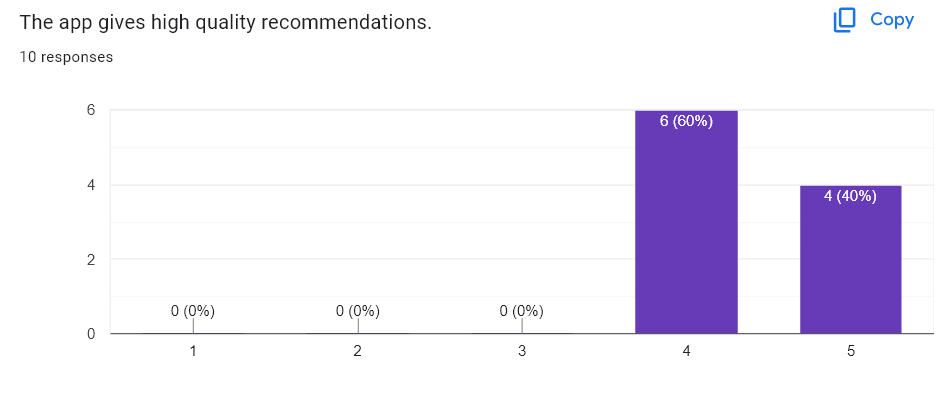
\includegraphics[width=1\textwidth]{images/Q1.png}
        \caption{Likert Scale Statement: ``The app gives high quality recommendations"}
        \label{fig:Q1}
    \end{subfigure}
    \hfill
    \begin{subfigure} [b] {0.49\textwidth}
        \centering
        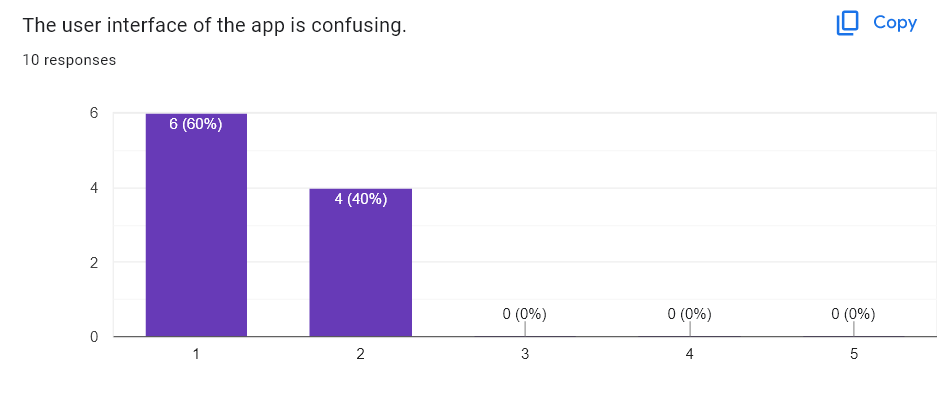
\includegraphics[width=1\textwidth]{images/Q2.png}
        \caption{Likert Scale Statement: ``The user interface of the app is confusing"}
        \label{fig:Q2}
    \end{subfigure}
    \hfill
    \begin{subfigure} [b] {0.49\textwidth}
        \centering
        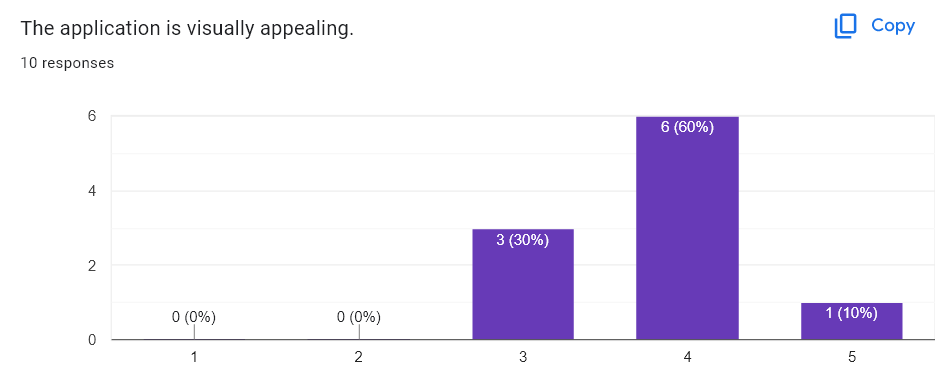
\includegraphics[width=1\textwidth]{images/Q3.png}
        \caption{Likert Scale Statement: ``The application is visually appealing"}
        \label{fig:Q3}
    \end{subfigure}
    \hfill
    \begin{subfigure} [b] {0.49\textwidth}
        \centering
        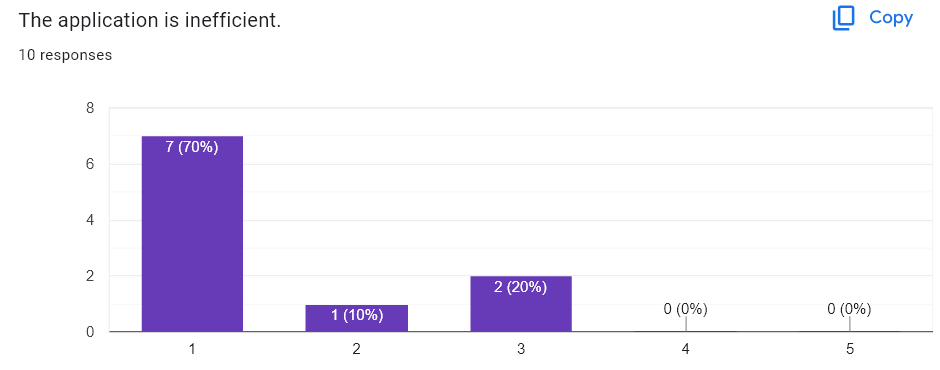
\includegraphics[width=1\textwidth]{images/Q4.png}
        \caption{Likert Scale Statement: ``The application is inefficient"}
        \label{fig:Q4}
    \end{subfigure}
    \hfill
    \begin{subfigure} [b] {0.49\textwidth}
        \centering
        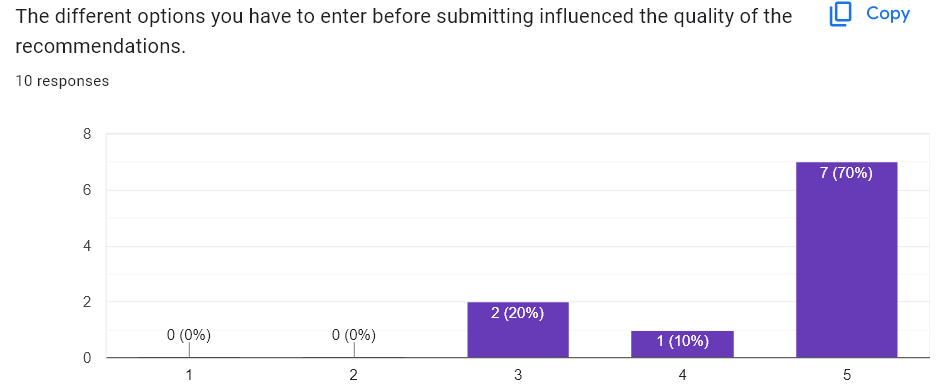
\includegraphics[width=1\textwidth]{images/Q5.png}
        \caption{Likert Scale Statement: ``The different options you have to enter before submitting influenced the quality of the recommendations"}
        \label{fig:Q5}
    \end{subfigure}
    \hfill
    \begin{subfigure} [b] {0.49\textwidth}
        \centering
        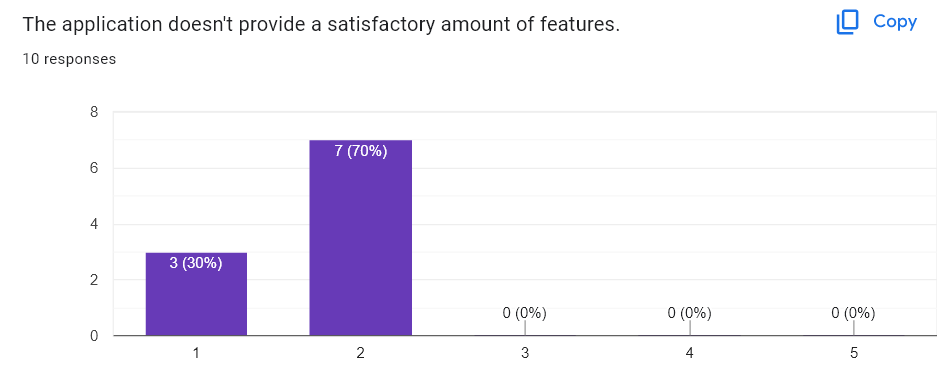
\includegraphics[width=1\textwidth]{images/Q6.png}
        \caption{Likert Scale Statement: ``The application doesn't provide a satisfactory amount of features"}
        \label{fig:Q6}
    \end{subfigure}
    \hfill
    \begin{subfigure} [b] {0.49\textwidth}
        \centering
        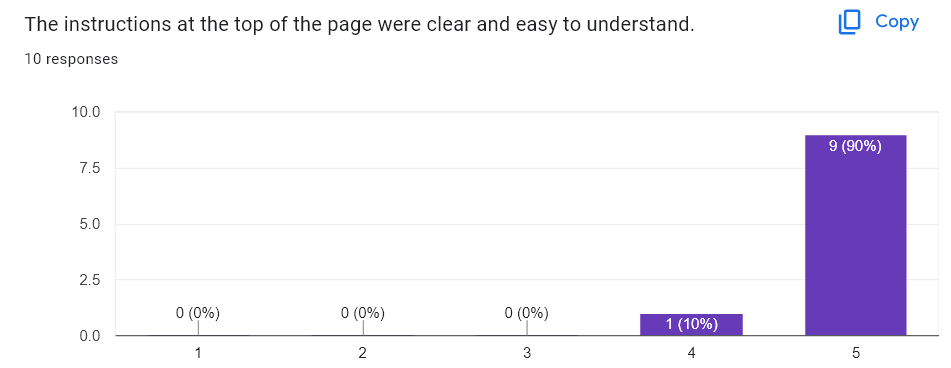
\includegraphics[width=1\textwidth]{images/Q7.png}
        \caption{Likert Scale Statement: ``The instructions at the top of the page were clear and easy to understand"}
        \label{fig:Q7}
    \end{subfigure}
    \hfill
    \begin{subfigure} [b] {0.49\textwidth}
        \centering
        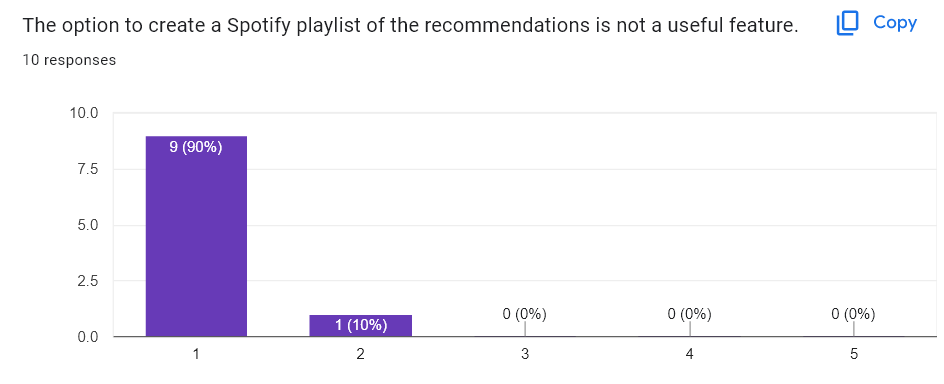
\includegraphics[width=1\textwidth]{images/Q8.png}
        \caption{Likert Scale Statement: ``The option to create a Spotify playlist of the recommendations is not a useful feature"}
        \label{fig:Q8}
    \end{subfigure}
    \hfill
    \begin{subfigure} [b] {0.49\textwidth}
        \centering
        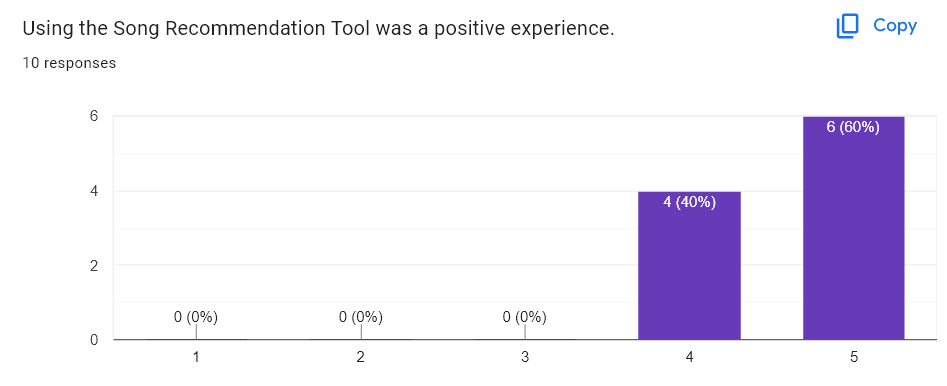
\includegraphics[width=1\textwidth]{images/Q9.png}
        \caption{Likert Scale Statement: ``Using the Song Recommendation Tool was a positive experience"}
        \label{fig:Q9}
    \end{subfigure}
    \hfill
    \begin{subfigure} [b] {0.49\textwidth}
        \centering
        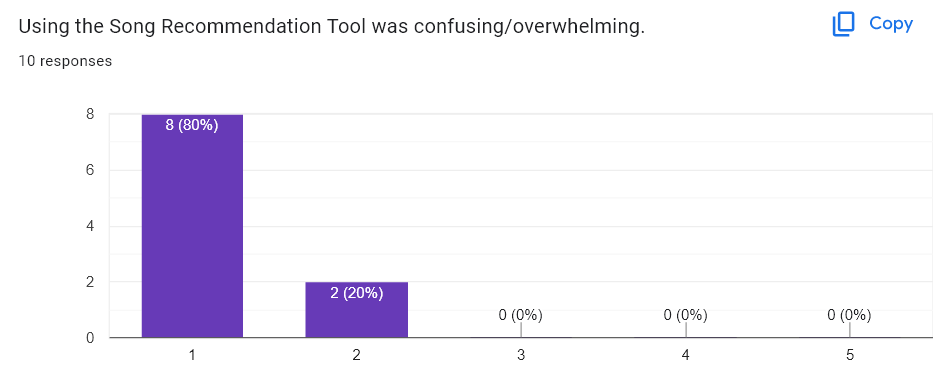
\includegraphics[width=1\textwidth]{images/Q10.png}
        \caption{Likert Scale Statement: ``Using the Song Recommendation Tool was confusing/overwhelming"}
        \label{fig:Q10}
    \end{subfigure}
    \hfill
    \begin{subfigure} [b] {0.49\textwidth}
        \centering
        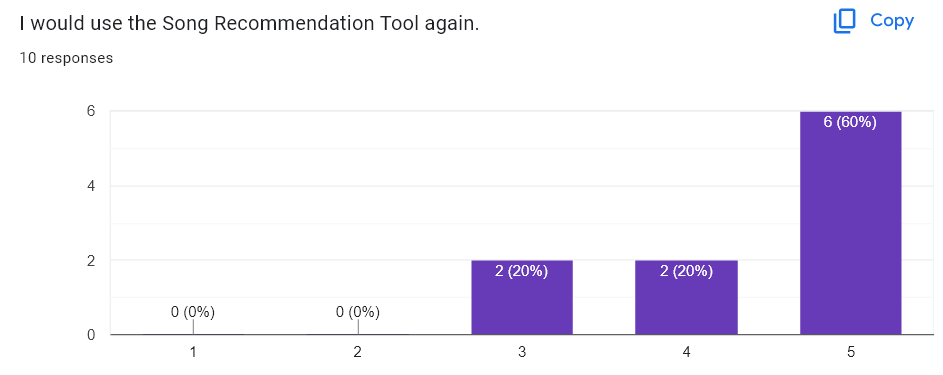
\includegraphics[width=1\textwidth]{images/Q11.png}
        \caption{Likert Scale Statement: ``I would use the Song Recommendation Tool again"}
        \label{fig:Q11}
    \end{subfigure}
    \caption{Survey Likert Scale Statement results}
    \label{fig:LSQuestions}
\end{figure}
\subsection{Likert Scale Statement: ``The app gives high quality recommendations"}
Responses to this statement are split almost evenly between "Agree" and "Strongly Agree", with a count of 6 and 4 respectively. Considering "Agree" as a value of 4 and "Strongly Agree" as a value of 5(This will be used for later statements as well, with "Strongly Disagree" corresponding to a value of 1, "Disagree" meaning 2, and "Neither Agree/Disagree" meaning 3), the average of these responses is 4.4, with a median of 4. These results indicate that participants generally believe that the Song Recommendation Tool gives high quality recommendations.
\subsection{Likert Scale Statement: ``The user interface of the app is confusing"}
Responses to this statement are split almost evenly between "Strongly Disagree" and "Disagree", with a count of 6 and 4 respectively. Statistics for this statement include a mean of 1.4, and a median of 1, indicating that participants generally believe that the user interface of the application is definitely not confusing.  
\subsection{Likert Scale Statement: ``The application is visually appealing"}
With the widest range of any of the Likert Scale Statements thus far, responses to this statement are split as 3 responses for "Neither Agree/Disagree", 4 responses for "Agree", and 1 response for "Strongly Agree". The statistics for this statement are a mean of 3.8 and a median of 4. Therefore, participants generally believe that the Song Recommendation Tool is visually appealing.
\subsection{Likert Scale Statement: ``The application is inefficient"}
Similarly to the previous statement, responses to this one are spread over three consecutive options. There are 7 responses for "Strongly Disagree", 1 response for "Disagree", and 2 responses for "Neither Agree/Disagree". The mean of these responses is 1.5, and the median is 1, showing that participants generally definitely disagree with the statement that the application is inefficient. 
\subsection{Likert Scale Statement: ``The different options you have to enter before submitting influenced the quality of the recommendations"}
Again with a range over three consecutive options, responses to this statement are 2 for "Neither Agree/Disagree", 1 for "Agree", and 7 for "Strongly Agree", leading to statistics of a mean of 4.5 and a median of 5. These results indicate that participants generally believe that the different parameters they enter before submitting definitely influence the quality of the recommendations they receive.
\subsection{Likert Scale Statement: ``The application doesn't provide a satisfactory amount of features"}
With a range of over two consecutive options, responses for this statement are 3 for "Strongly Disagree" and 7 for "Disagree", resulting in a mean of 1.7 and a median of 2. That means that participants generally disagree with the statement that the application doesn't provide a satisfactory amount of features.
\subsection{Likert Scale Statement: ``The instructions at the top of the page were clear and easy to understand"}
Tied with the next question for highest number of responses for a single option, the responses for this statement are 1 for Agree and a resounding 9 for Strongly Agree. This leads to a mean of 4.9 and a mean of 5, which surely indicate that participants generally believe that the instructions at the top of the page were most definitely clear and easy to understand.
\subsection{Likert Scale Statement: ``The option to create a Spotify playlist of the recommendations is not a useful feature"}
Over a range of two consecutive options, there are 9 responses for "Strongly Disagree" and 1 response for "Disagree" when it comes to this statement. The statistics that can be extracted are a mean of 1.1 and a median of 2. Consequently, participants generally certainly disagree with the statement that the option of Spotify playlist creation is not a useful feature.
\subsection{Likert Scale Statement: ``Using the Song Recommendation Tool was a positive experience"}
Returning to the early results of almost evenly split responses, this statement yielded 4 responses for "Agree" and 6 responses for "Strongly Agree", leading to a mean of 4.6 and a median of 5. These statistics show that participants generally believe that using the Song Recommendation Tool was most certainly a positive experience.
\subsection{Likert Scale Statement: ``Using the Song Recommendation Tool was confusing/overwhelming"}
Responses to this statement are 8 for "Strongly Disagree" and 2 for "Disagree". The mean for these results is 1.2, and the median is 1, meaning that participants generally absolutely disagree that using the Song Recommendation Tool was a confusing or overwhelming experience.
\subsection{Likert Scale Statement: ``I would use the Song Recommendation Tool again"}
Ranging over three consecutive options, the responses for the final Likert Scale Statement are: 2 responses for "Neither Agree/Disagree", 2 responses for "Agree", and 6 responses for "Strongly Agree". The mean for these results is 4.4, while the median has a value of 5, indicating that participants would most probably use the Song Recommendation Tool again.
\subsection{Long-Form Text Input Question: ``Are there any features you would like to see implemented in the application?"}
After collecting 8 responses out of 10 participants for this open-ended question, the results are summarised in this subsection. The most common suggestions were to implement a way to preview/listen to songs on the website itself, and to implement a way to avoid recommending songs the user already likes or has listened to before. Other suggestions were to improve the search system to autocomplete the user's input or to suggest potential songs the user is trying to input, and to potentially recommend albums and playlists as well as songs. Finally, as far as the Create a Spotify Playlist feature is concerned, participants suggested that they would like the option to add recommendations to an already-existent playlist, and to have the option to exclude some of the recommended songs from being added to a playlist.
\subsection{Long-Form Text Input Question: ``Did you encounter any issues of any kind throughout your experience using the application?"}
With 9 responses collected to this question, this subsection contains a summary of the results. While 5 of the responses outlined that there were no issues encountered, other responses indicated the following issues: As mentioned in the Limitations section of the Implementation chapter, songs sometimes would not be found, or would not have genre tags attached to them. Moreover, one participant noted that the application was a bit slow(although they mentioned that they appreciated that it could be due to multiple factors), with the same participant also noting that they felt like the ``tags to prioritise" parameter did not influence their recommendations much.
\subsection{Long-Form Text Input Question: ``Please comment on if you consider the application useful"}
Again, 9 responses were collected for this question, and the main themes from the very useful feedback are contained in this subsection. Firstly, most participants stated that the application was useful, giving reasons such as that it helped them explore new artists, genres, and songs, that it got them out of their current listening habits, and that they got recommendations for genres they have trouble finding new music for. Another participant noted that the Song Recommendation Tool has the potential to be a cool way to discover music and that it gives suitable recommendations, although they are unsure if it is enough to outdo the mainstream competition. Finally, multiple participants stated that they would use the Song Recommendation Tool again.
\section{Evaluation Reflection}
Multiple sentiments and outcomes can be extracted from all the data points collected from the Evaluation questions. A general statement that can be made about the Song Recommendation Tool is that while not all of its aspects are excellent or to the level of its potential competitors, the Song Recommendation Tool could still be greater with some more work. Some of the greatest qualities of the Song Recommendation Tool, according to the evaluation participants, seem to be the user interface's simplicity, the application's efficiency, the different input parameters, the clear instructions at the top of the page, and the Create a Spotify Playlist feature. Participants overall claimed that using the Song Recommendation Tool was a positive and simple experience and that they would use the application again. From the qualitative responses, there are also various ways suggested to improve the Song Recommendation Tool. Participants would like input to be even more customizable, and for the song input to be more intuitive and user-friendly, perhaps more similar to mainstream music services that offer suggestions during input. In addition, the suggestion made by participants to include the option for songs to be listenable inside the Song Recommendation Tool would be a significant extension to the implementation and scope of the project. An essential improvement would be to implement the suggestion that songs the user already knows/likes/has listened to would not be recommended to them. While this was discussed in the Limitation section of the implementation chapter, it is unfortunate that users had to encounter the drawbacks of using the Last.fm API as the main data source(songs not being found, songs not having tags attached to them). Furthermore, while it is not something participants would notice, it was great to see that more recent songs were found and were properly classified, something that another dataset would perhaps not be able to accomplish. Finally, when it comes to the evaluation procedure itself, it would certainly be an improvement if participants had longer-term access to the application, to allow observations of their experiences after using the Song Recommendation Tool multiple times.
%==================================================================================================================================
\chapter{Conclusion}

\section{Summary}
As discussed in-depth in the Background chapter, Recommender Systems are being included in many different modern products and services. One subset of these systems is Music Recommender Systems. Most competitive music platforms have integrated Music Recommender Systems into their products to streamline the process of music discovery and to keep users engaged in their services. These systems can collect large amounts of user data, and prioritising keeping users engaged with an application could potentially hinder the actual quality of the recommendations as users could be overwhelmed by the ways music is recommended to them or by the amount of music recommended to them. This project aimed was to develop a user-friendly application with the sole focus of giving users music recommendations based on their explicit preferences, without collecting any other amount of their data.\\[8pt]
When it comes to design, there is a visible split between the design philosophies of the Front-end and the Back-end. The Front-end focuses on simplicity, and on being user-friendly and easily understandable while sporting a sleek look. Data is processed and recommendations are derived in the much more complex Back-end. Included in the Back-end are many interconnected functions, with each one serving its own purpose. Front-end and Back-end are connected to allow the exchange of information between them.\\[8pt]
For the process of actually implementing the Song Recommendation Tool, some of the technologies and frameworks used were React, Flask, and Python. Music data was sourced via the Last.fm API to allow the use of more recent data, and to introduce another collaborative-based filtering aspect to the application, which also means that the Song Recommendation Tool is a lightweight application as there is no need to store massive volumes of data. The Front-end implementation is mostly comprised of song components, input fields, useState functions, and communication requests with the Back-end, which includes various functions that operate on the user's input, build up the user's profile, derive recommendations, and potentially create a Spotify playlist. Python was a very appropriate choice for the Data Science required to calculate to process data and calculate which tracks are best to be recommended.\\[8pt]
A very important part of the process of completing this project was assessing the quality of the Song Recommendation Tool by conducting evaluations and gathering feedback on participants' experiences with the application. Through pre-arranged sessions with 10 participants, the evaluation procedure involved completing two cycles of application use, listening to the recommendations, and completing a survey. Results were mostly positive, with high points being the simplicity and efficiency of the experience, with participants generally believing that they would use the application again to get new recommendations. Moreover, participants generally believed that the recommendations delivered by the application were high-quality. There were also many useful suggestions on future features that could make the Song Recommendation Tool even more appealing and competitive.\\[8pt]

\section{Future Work}
This section includes the future enhancements that could be made to further improve the quality of the Song Recommendation Tool.
\begin{itemize}
    \item Consider the user's listening history which could be provided by another source to avoid recommending songs they already know/listen to.
    \item Allow the user to preview/fully listen to songs that the application recommends to them.
    \item Autocomplete user input, or show suggestions for what the user could be trying to input while they are typing.
    \item Recommend artists, albums, and other playlists, not just songs.
    \item Extend input customisability(e.g. only allow recommendations from some of the artists the user inputs).
    \item Feature to add recommendations to an existing Spotify playlist.
\end{itemize}
%==================================================================================================================================
%
% 
%==================================================================================================================================
%  APPENDICES  

\begin{appendices}

\chapter{Evaluation Participant Consent Forms}
Start on the next page.

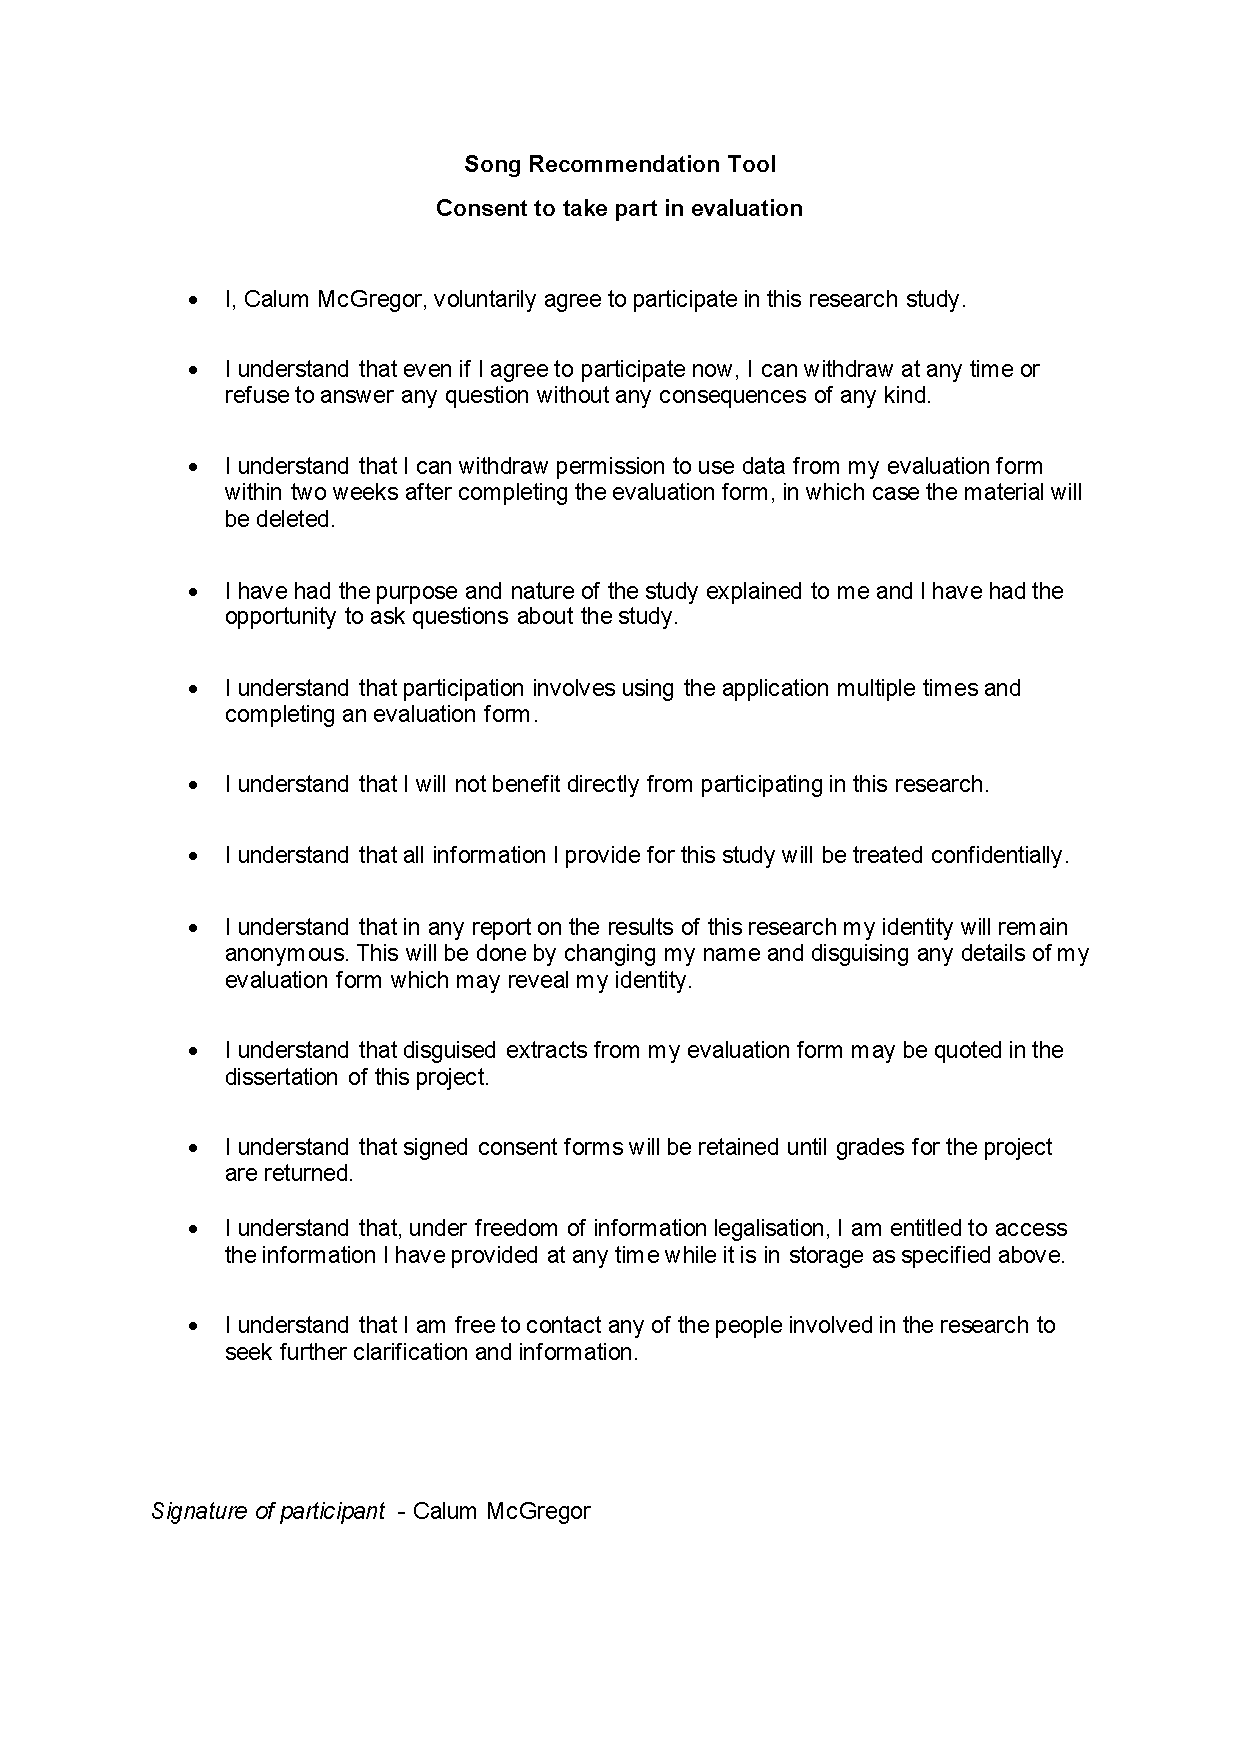
\includepdf[page={1,2}]{appendices/ConsentFormCal}
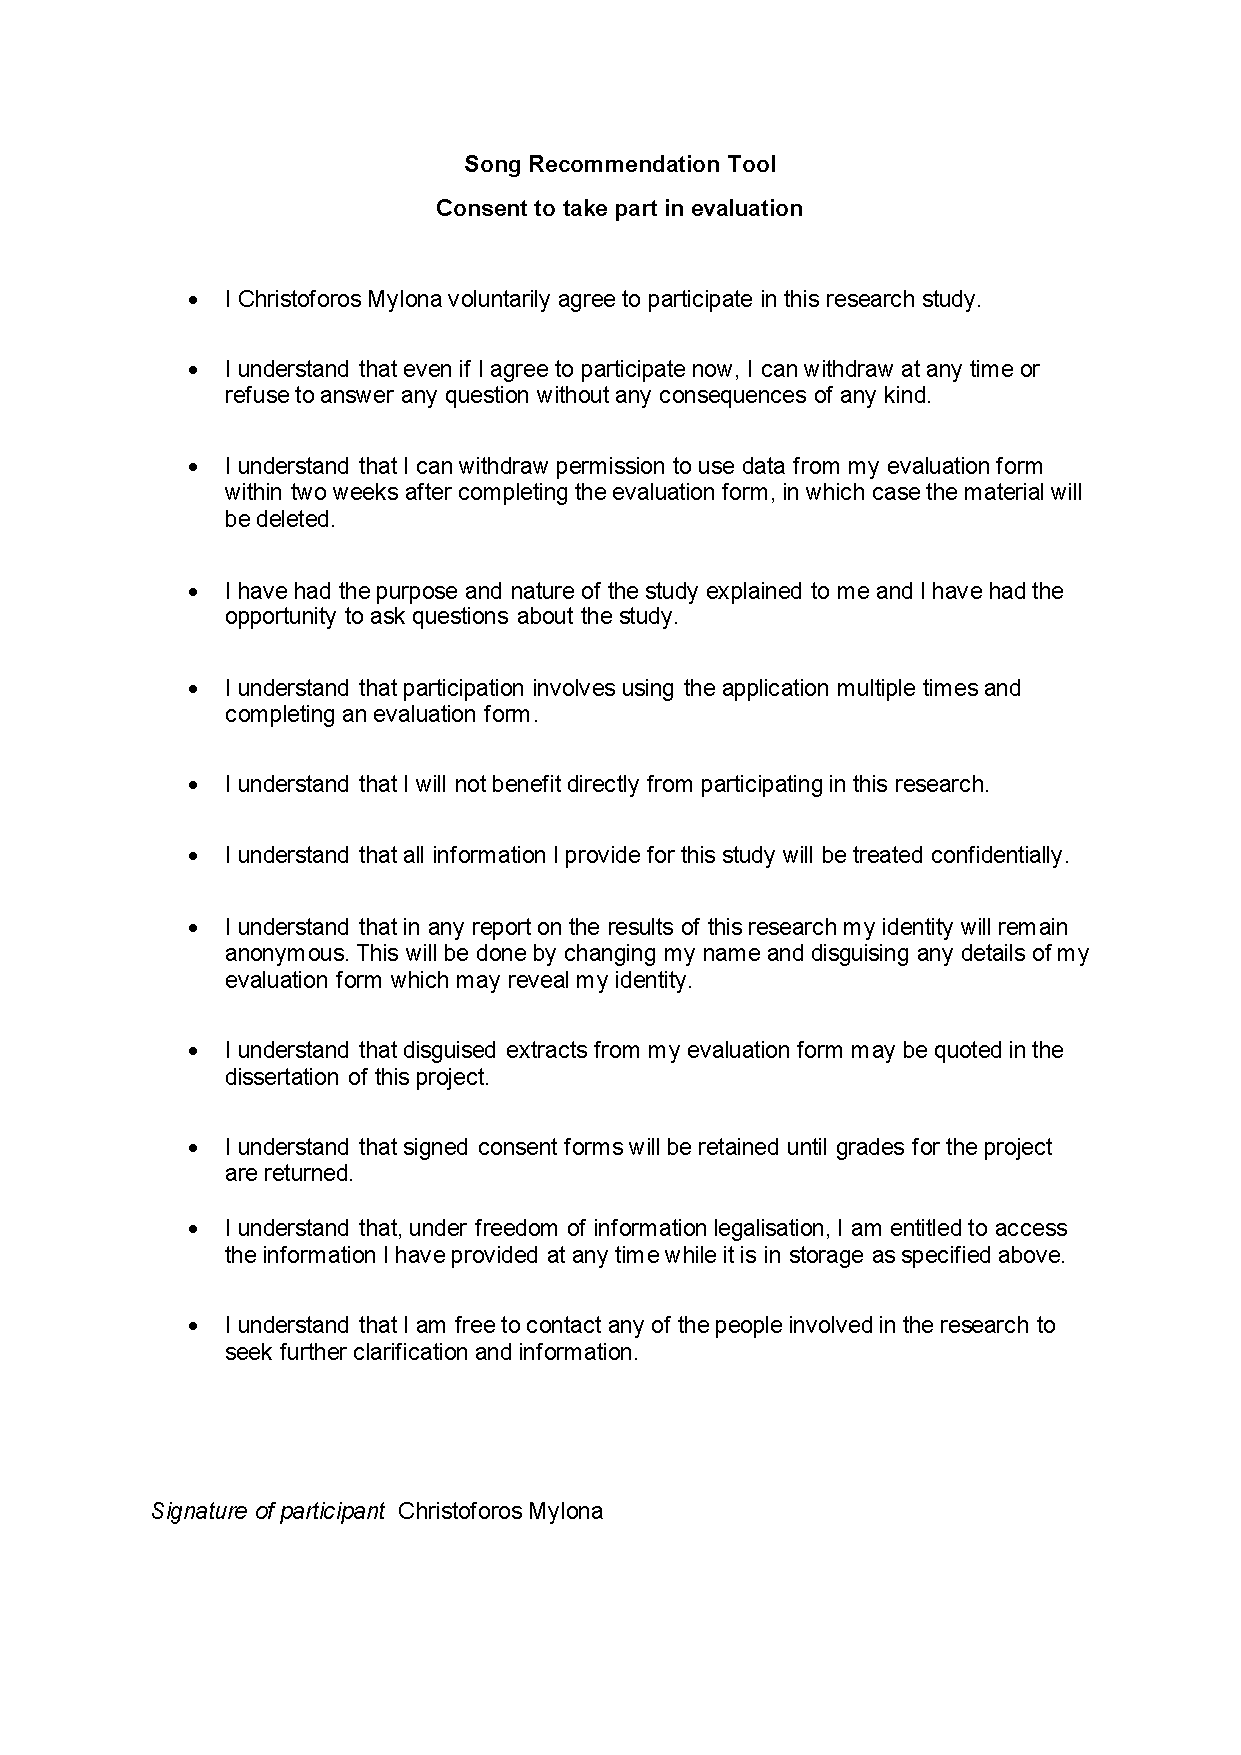
\includepdf[page={1,2}]{appendices/ConsentFormChris}
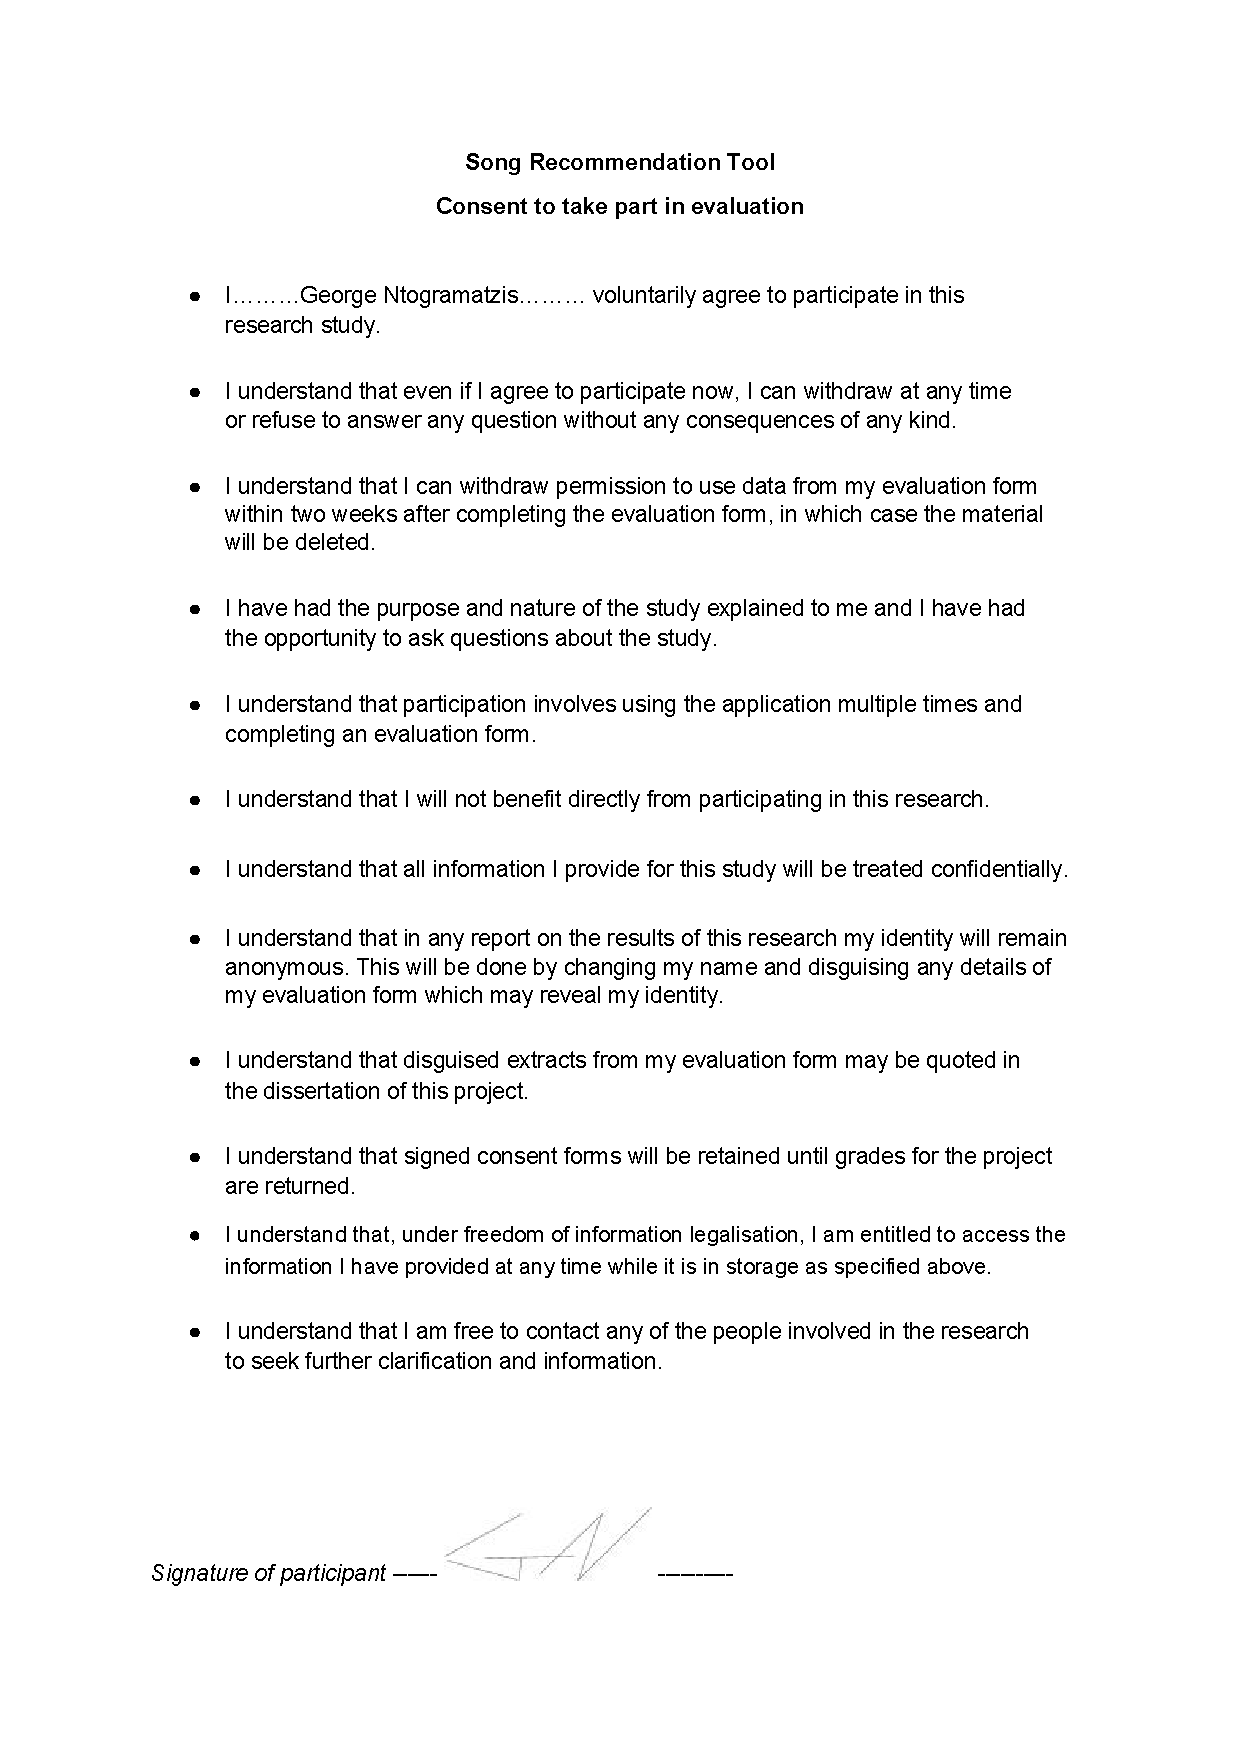
\includepdf[page={1,2}]{appendices/ConsentFormGeorge}
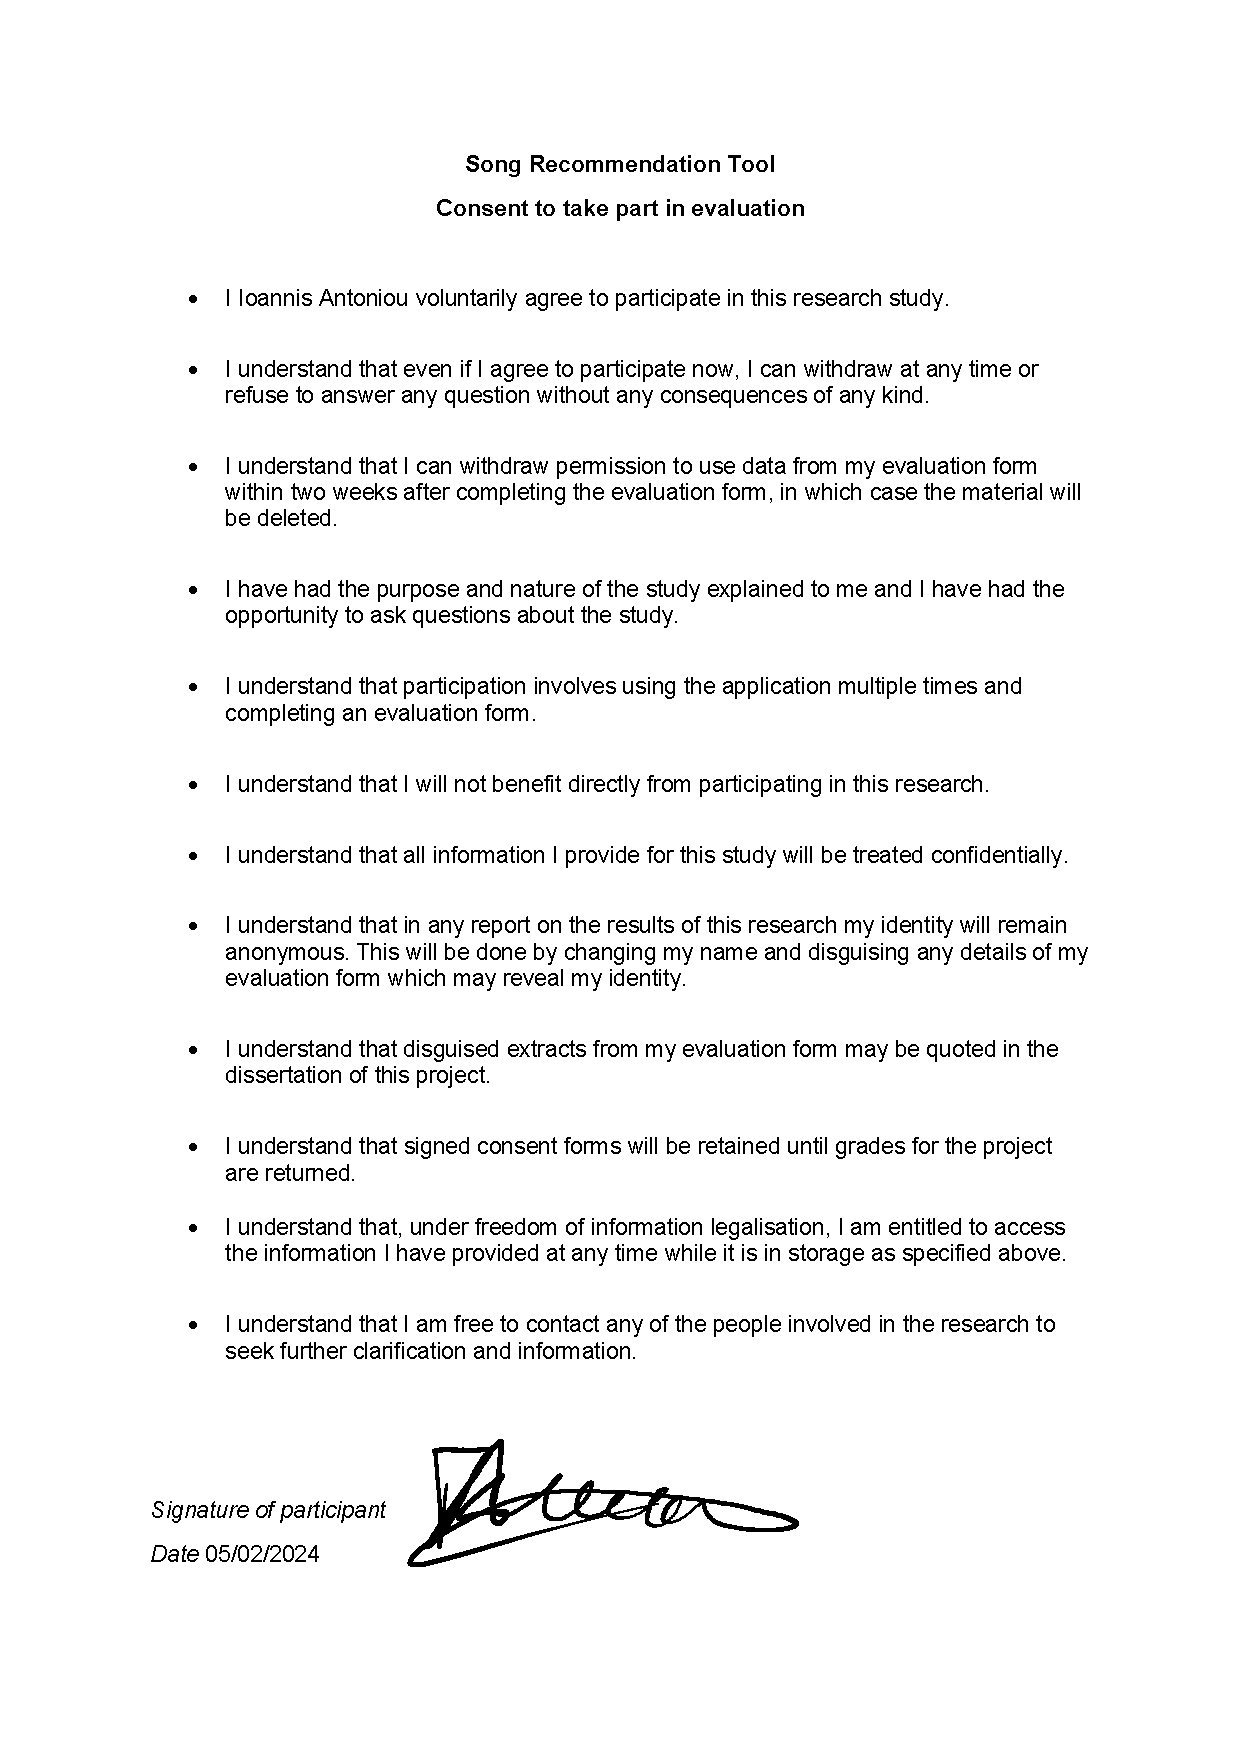
\includepdf[page={1,2}]{appendices/ConsentFormGiannis}
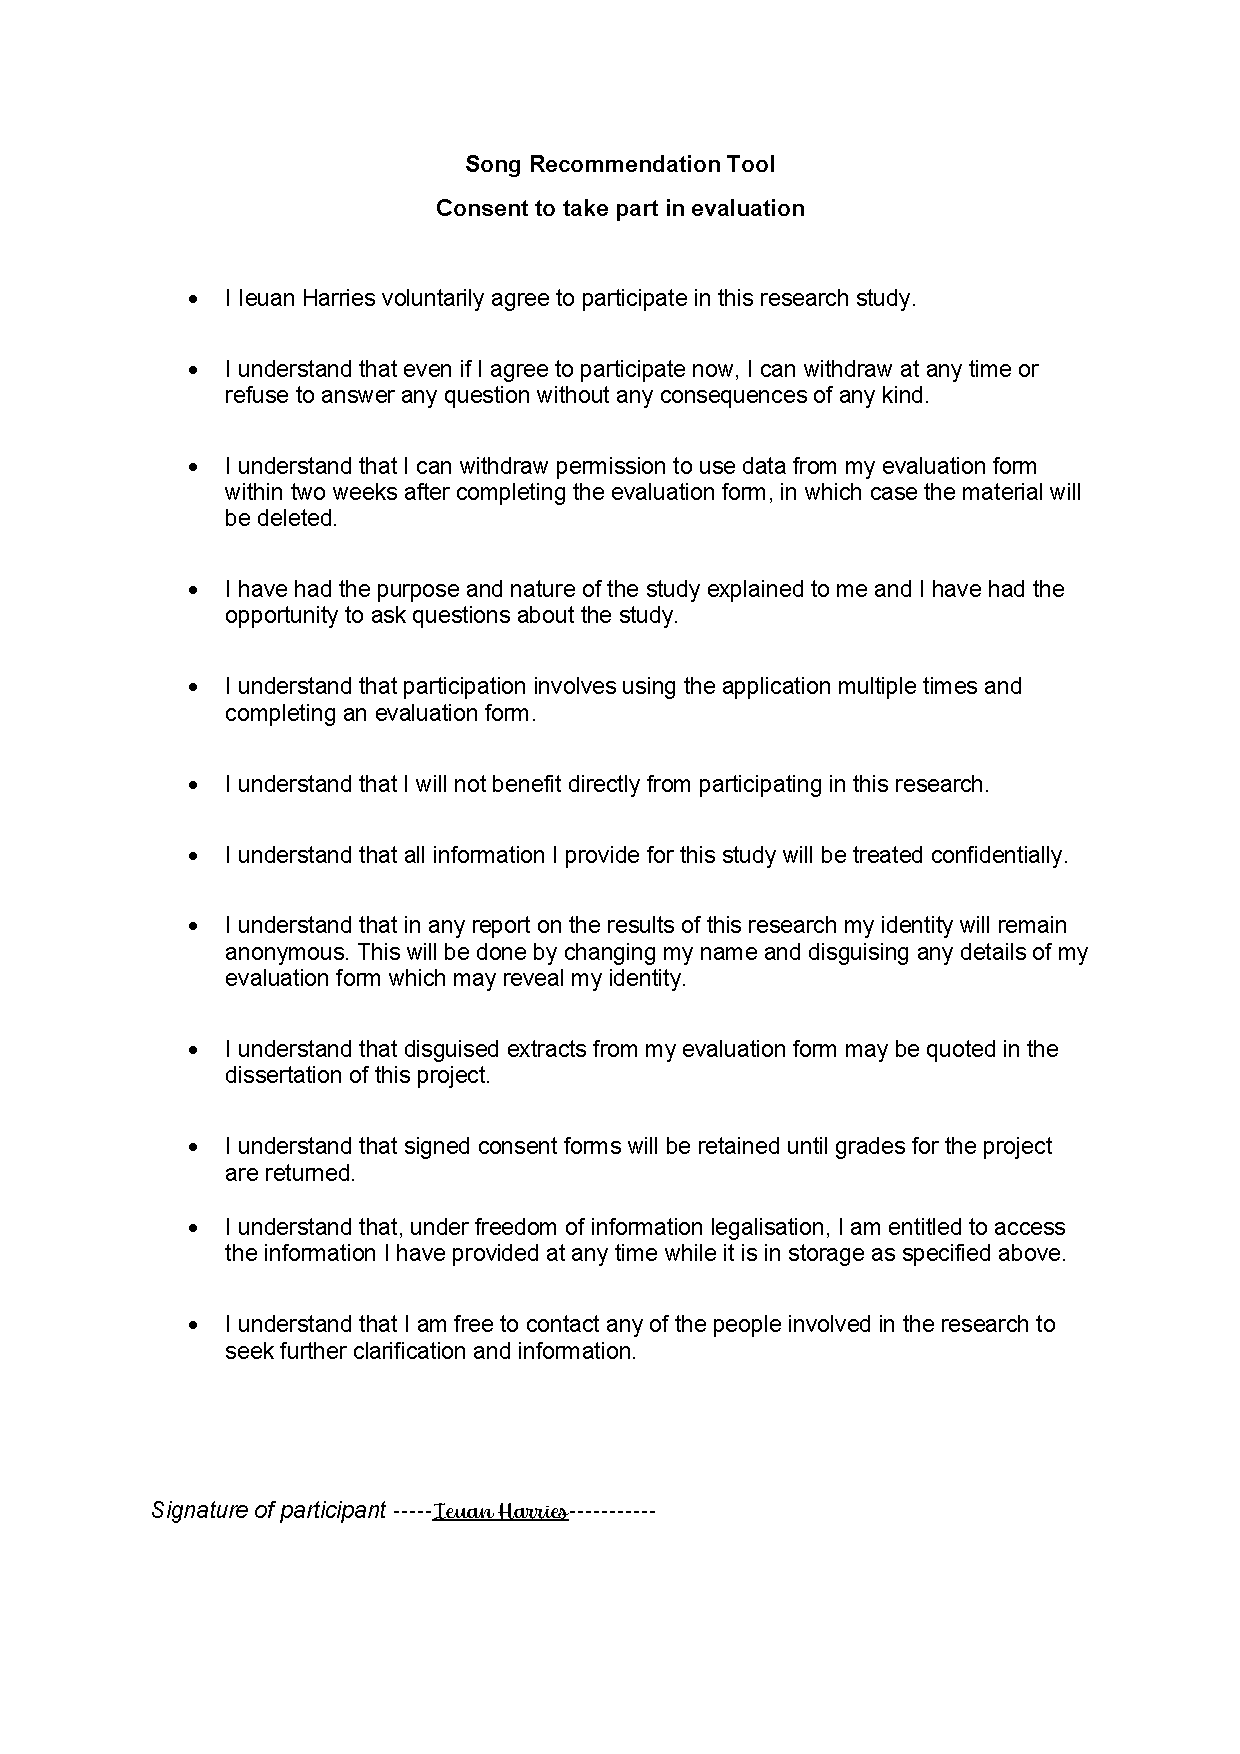
\includepdf[page={1,2}]{appendices/ConsentFormIeuan}
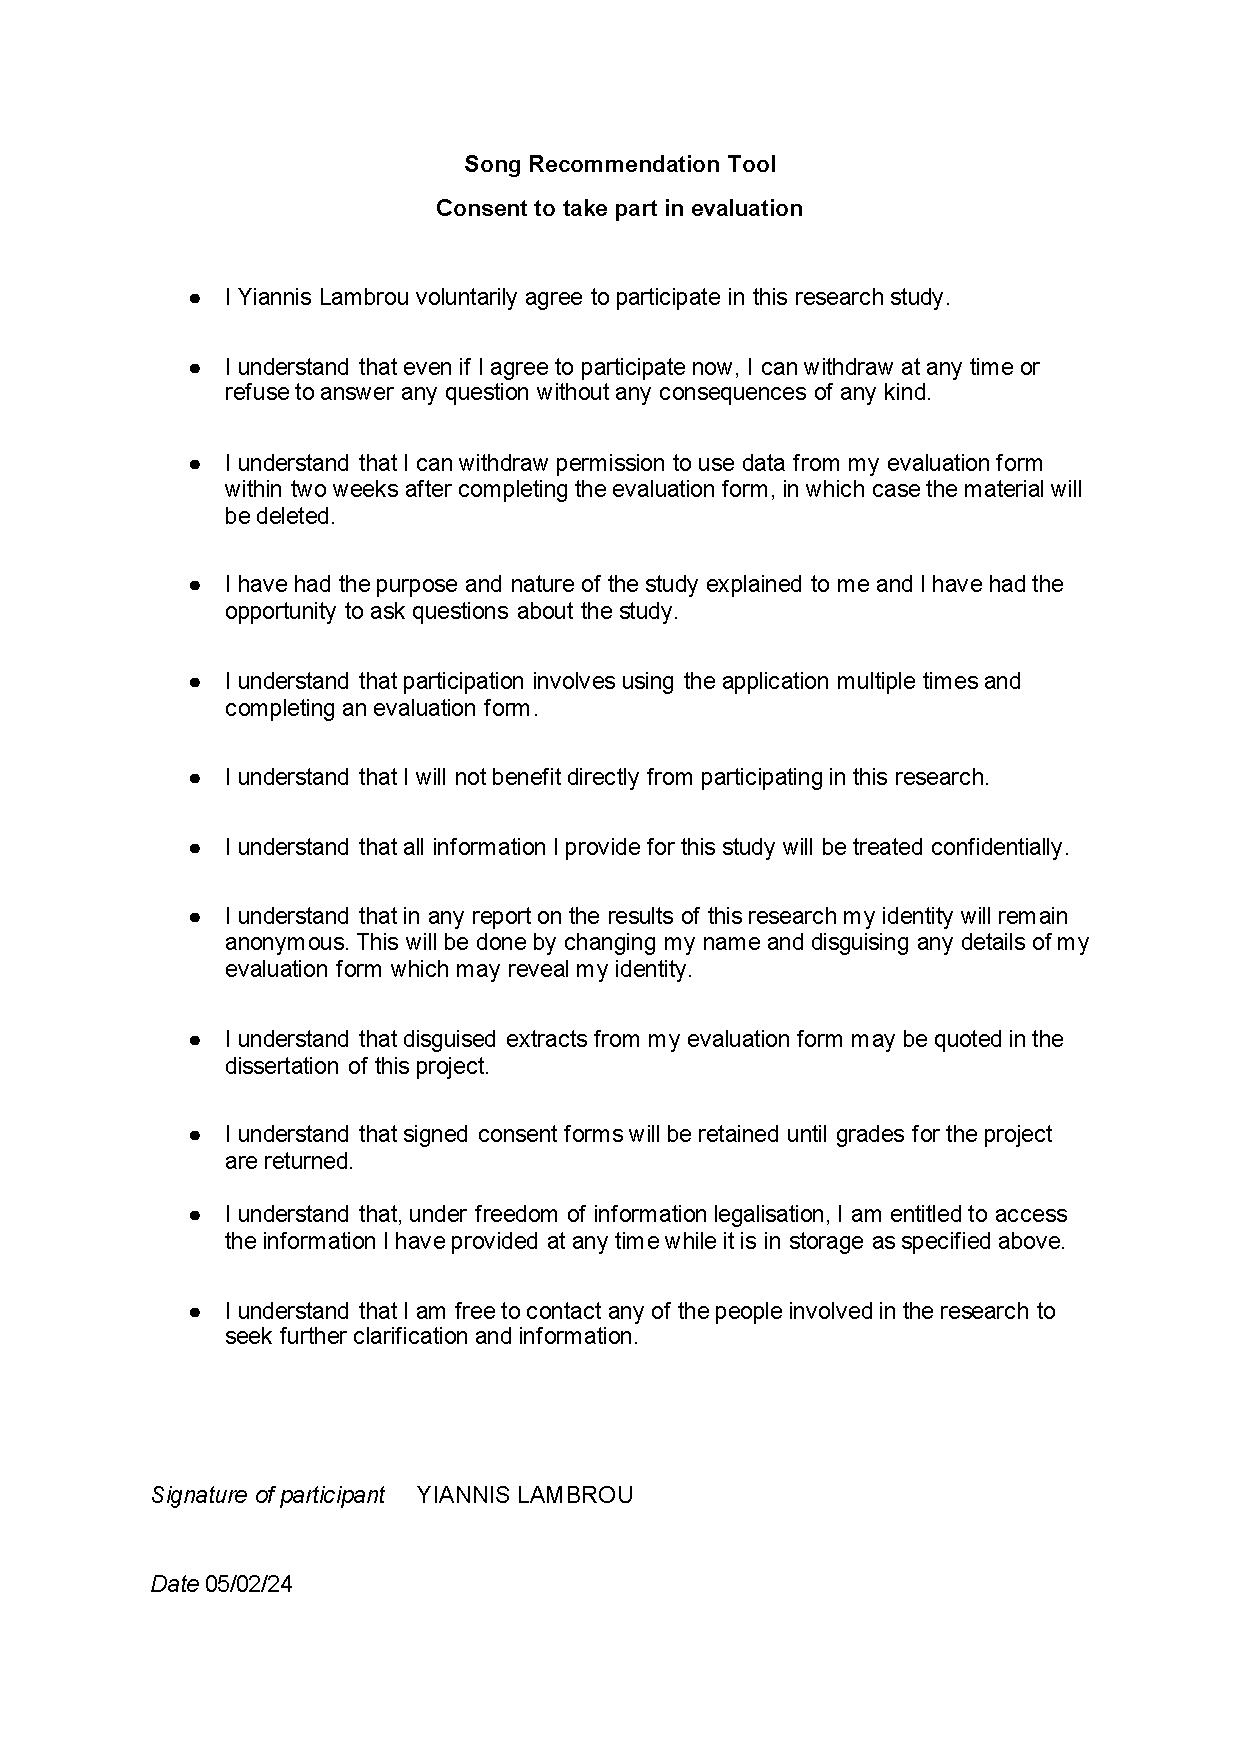
\includepdf[page={1,2}]{appendices/ConsentFormLam}
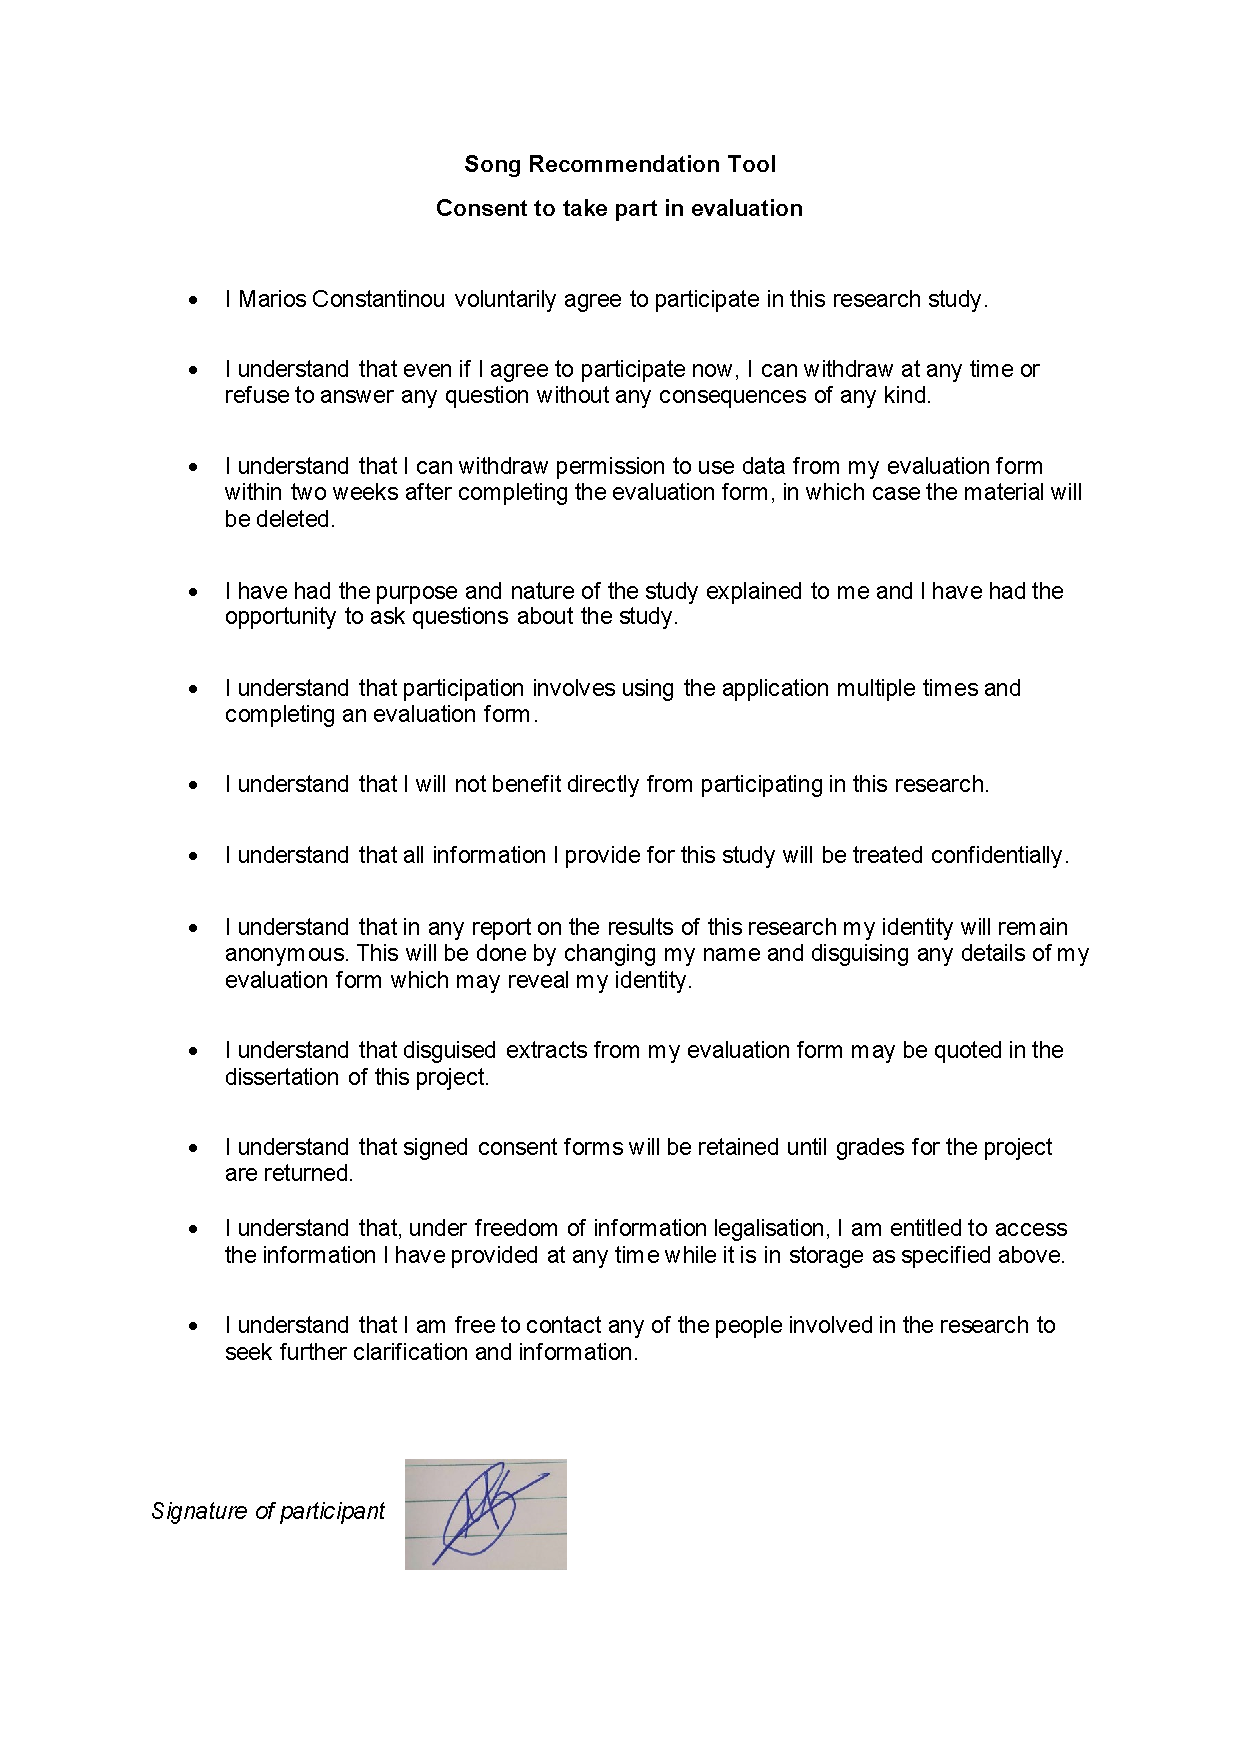
\includepdf[page={1,2}]{appendices/ConsentFormMarios}
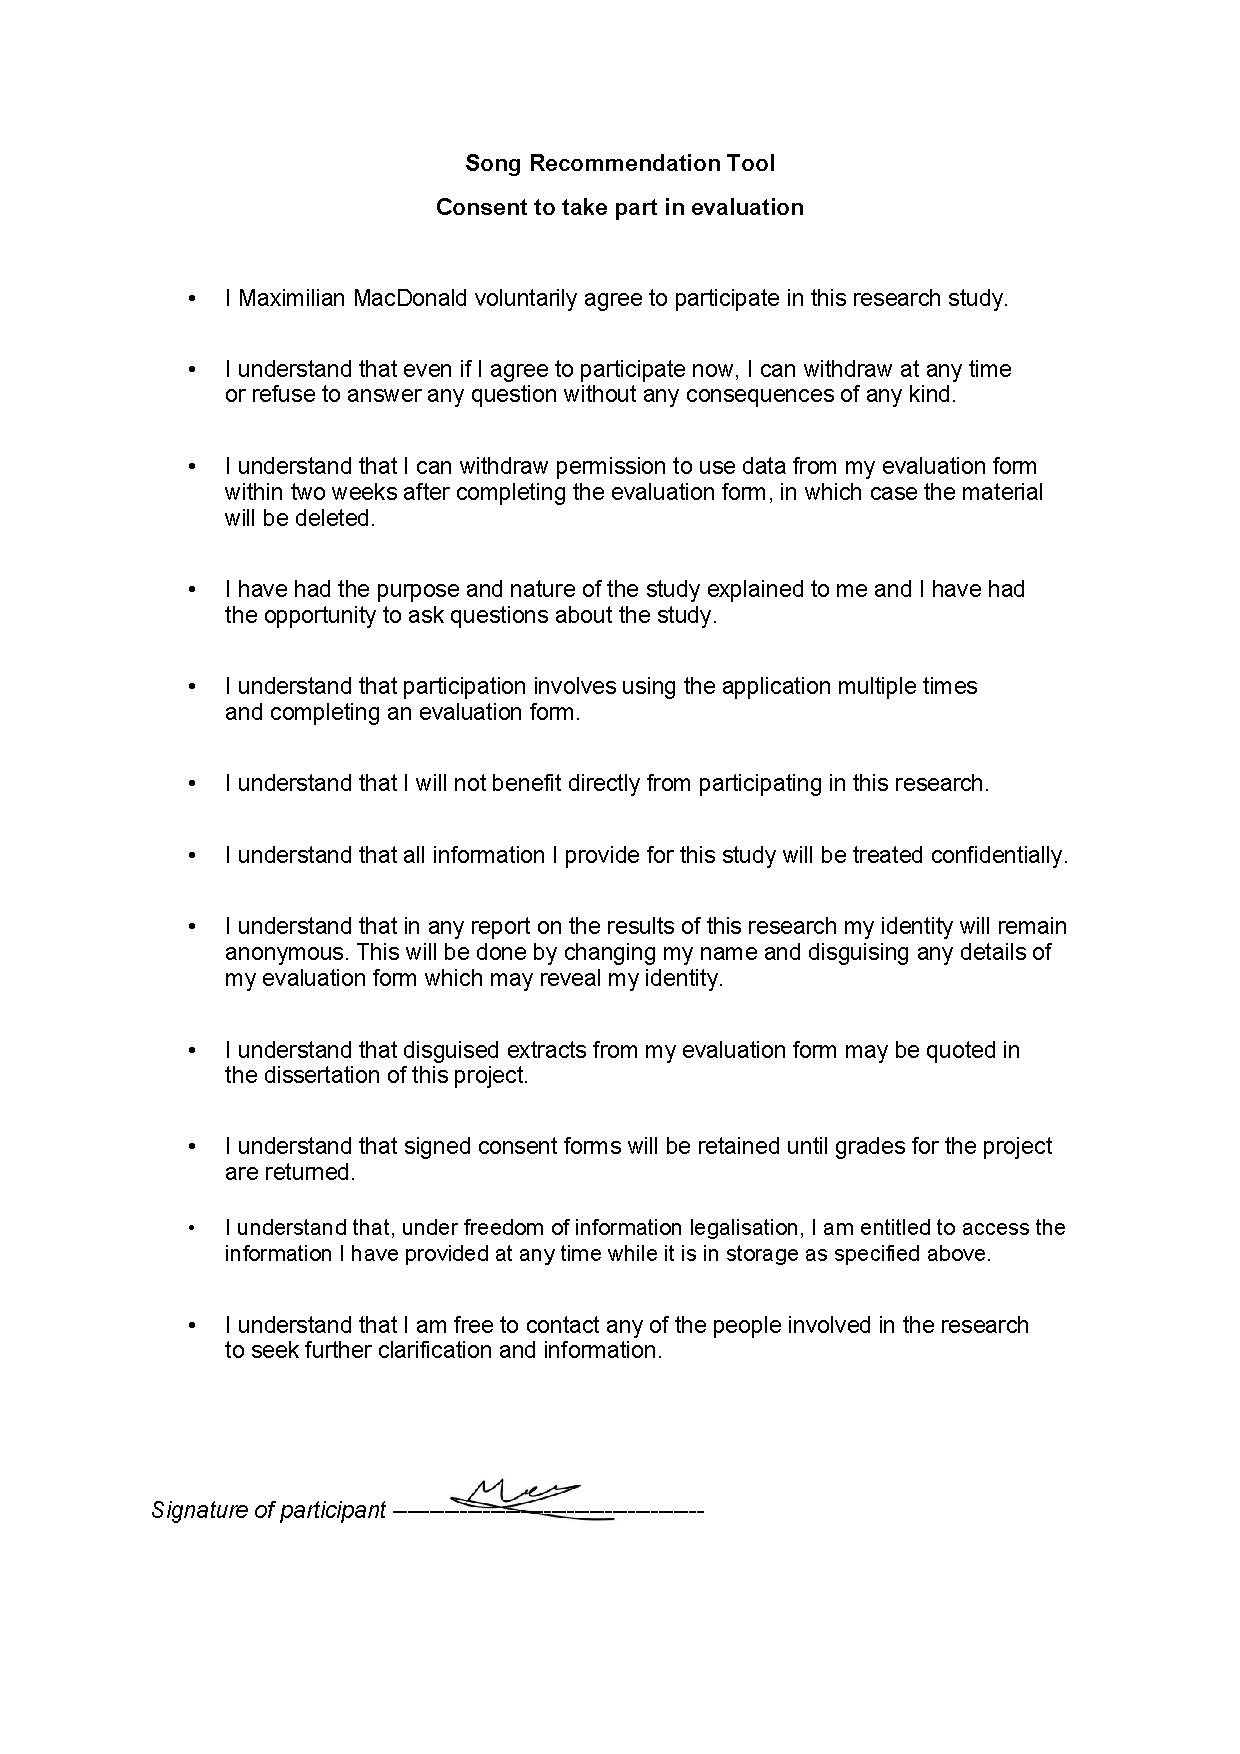
\includepdf[page={1,2}]{appendices/ConsentFormMax}
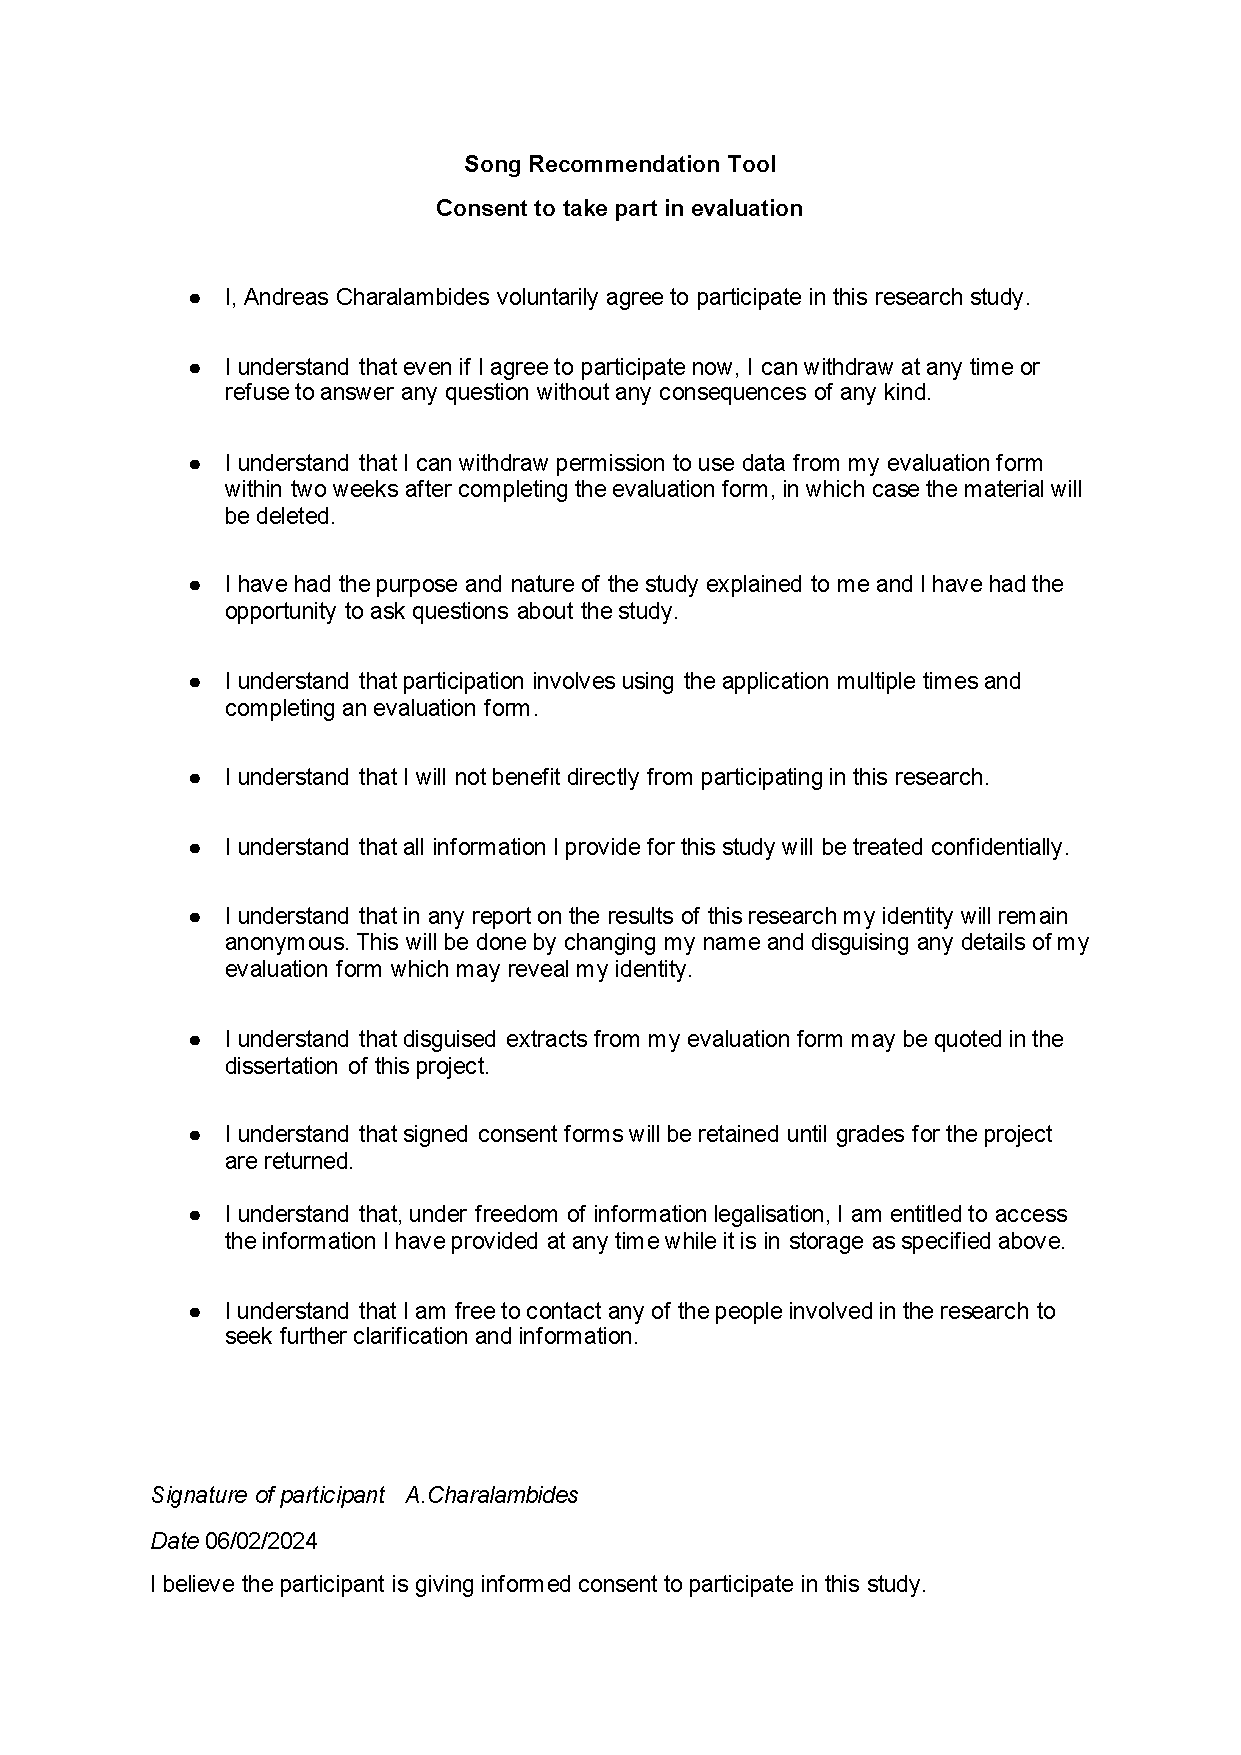
\includepdf[page={1,2}]{appendices/ConsentFormMbides}
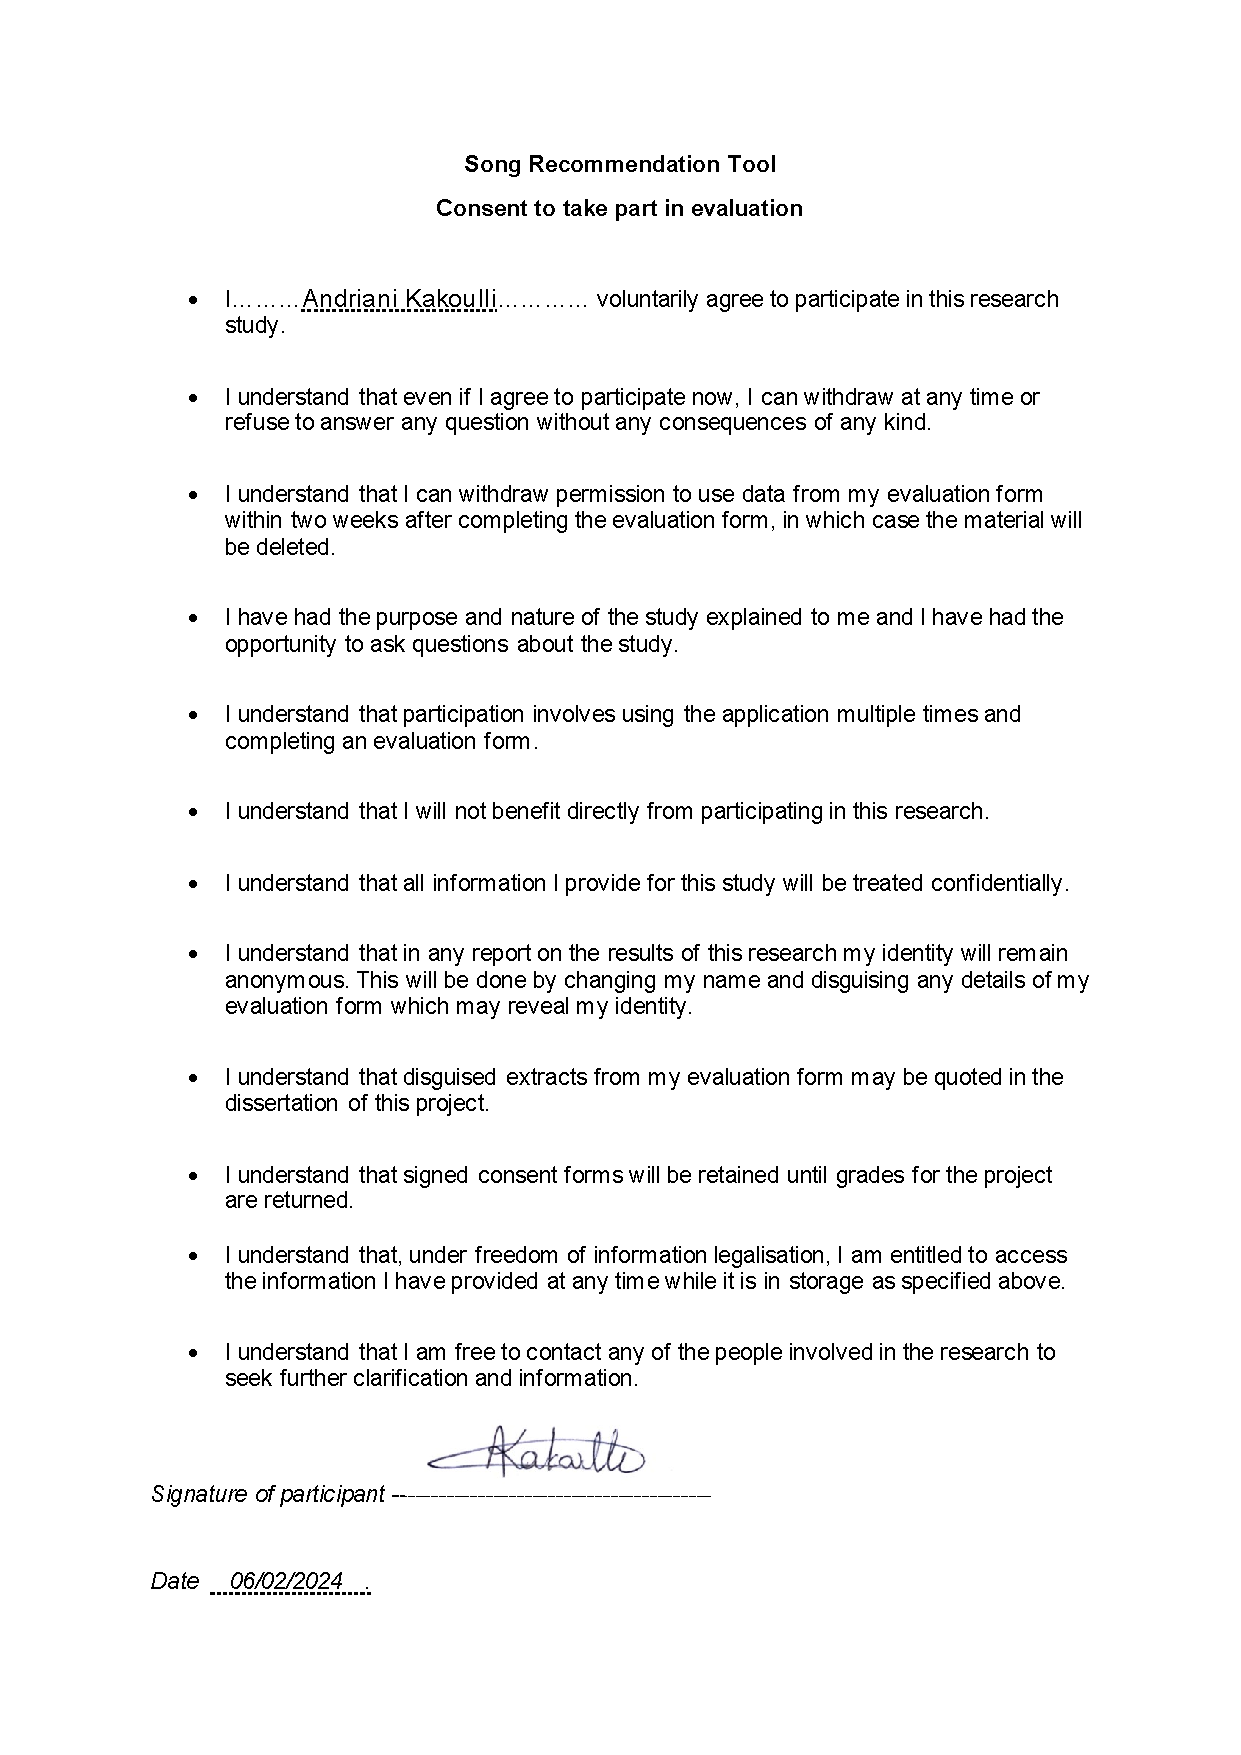
\includepdf[page={1,2}]{appendices/ConsentFormNoulla}

\chapter{Evaluation Ethics Checklist}
Start on next page.
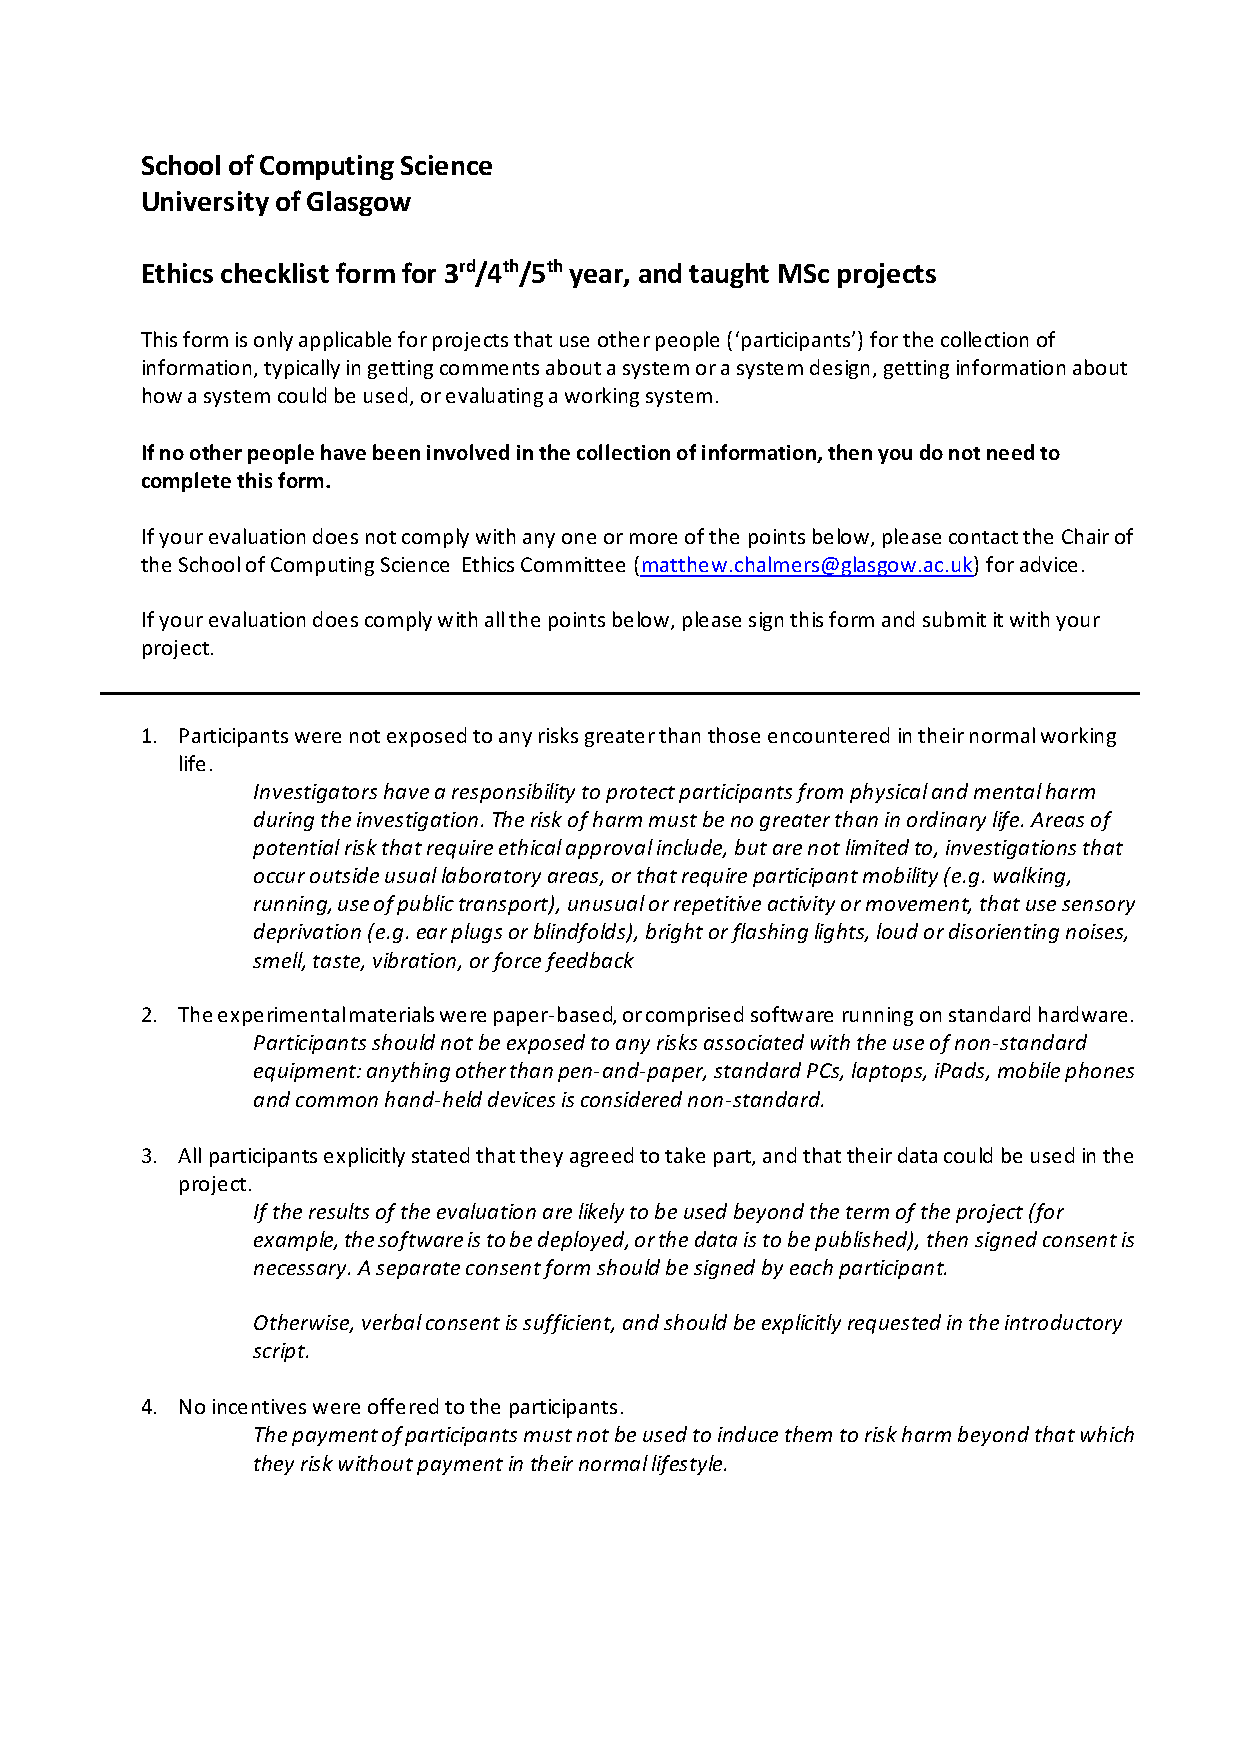
\includepdf[page={1,2}]{appendices/EvaluationEthicsChecklists}

\chapter{Evaluation Survey Responses}
Start on next page.
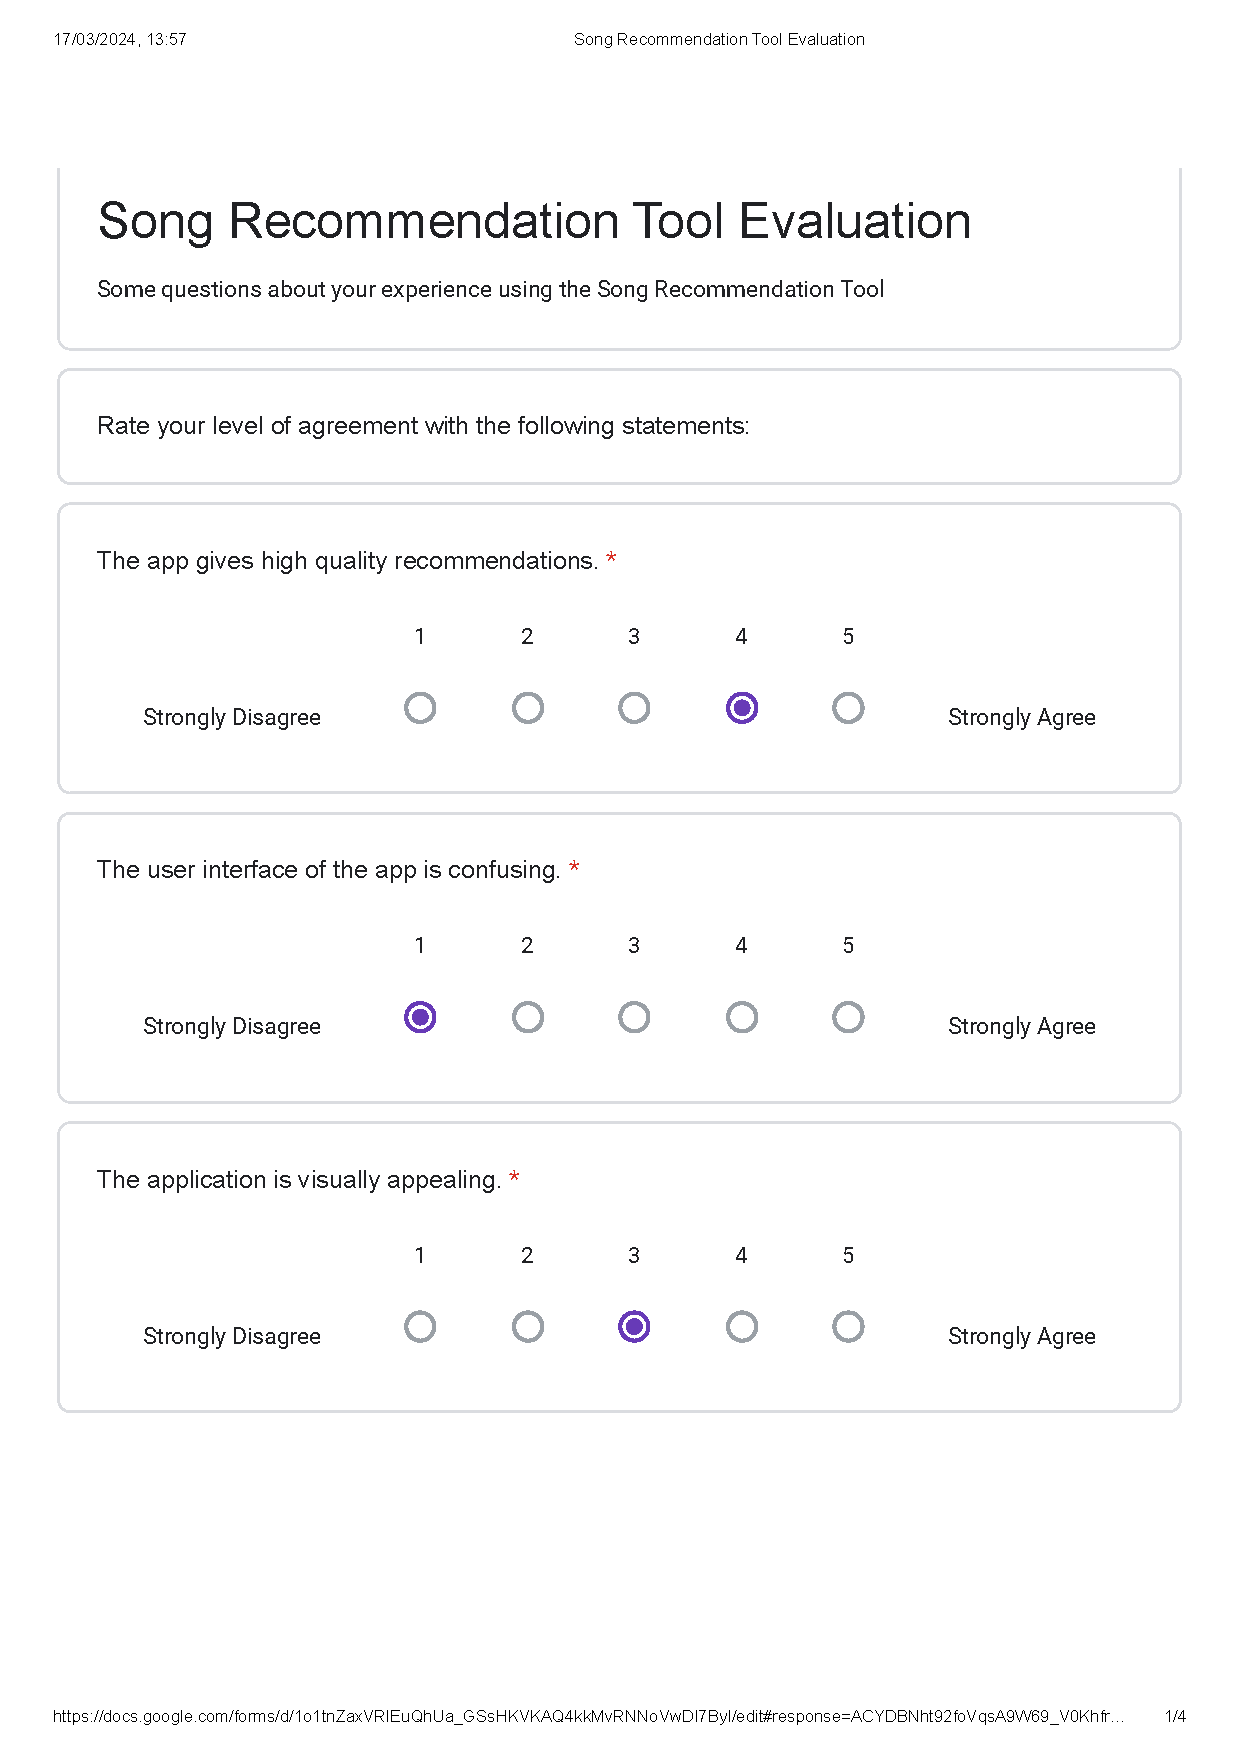
\includepdf[page={1,2,3,4}]{appendices/Song Recommendation Tool Evaluation - Google Forms - 1}
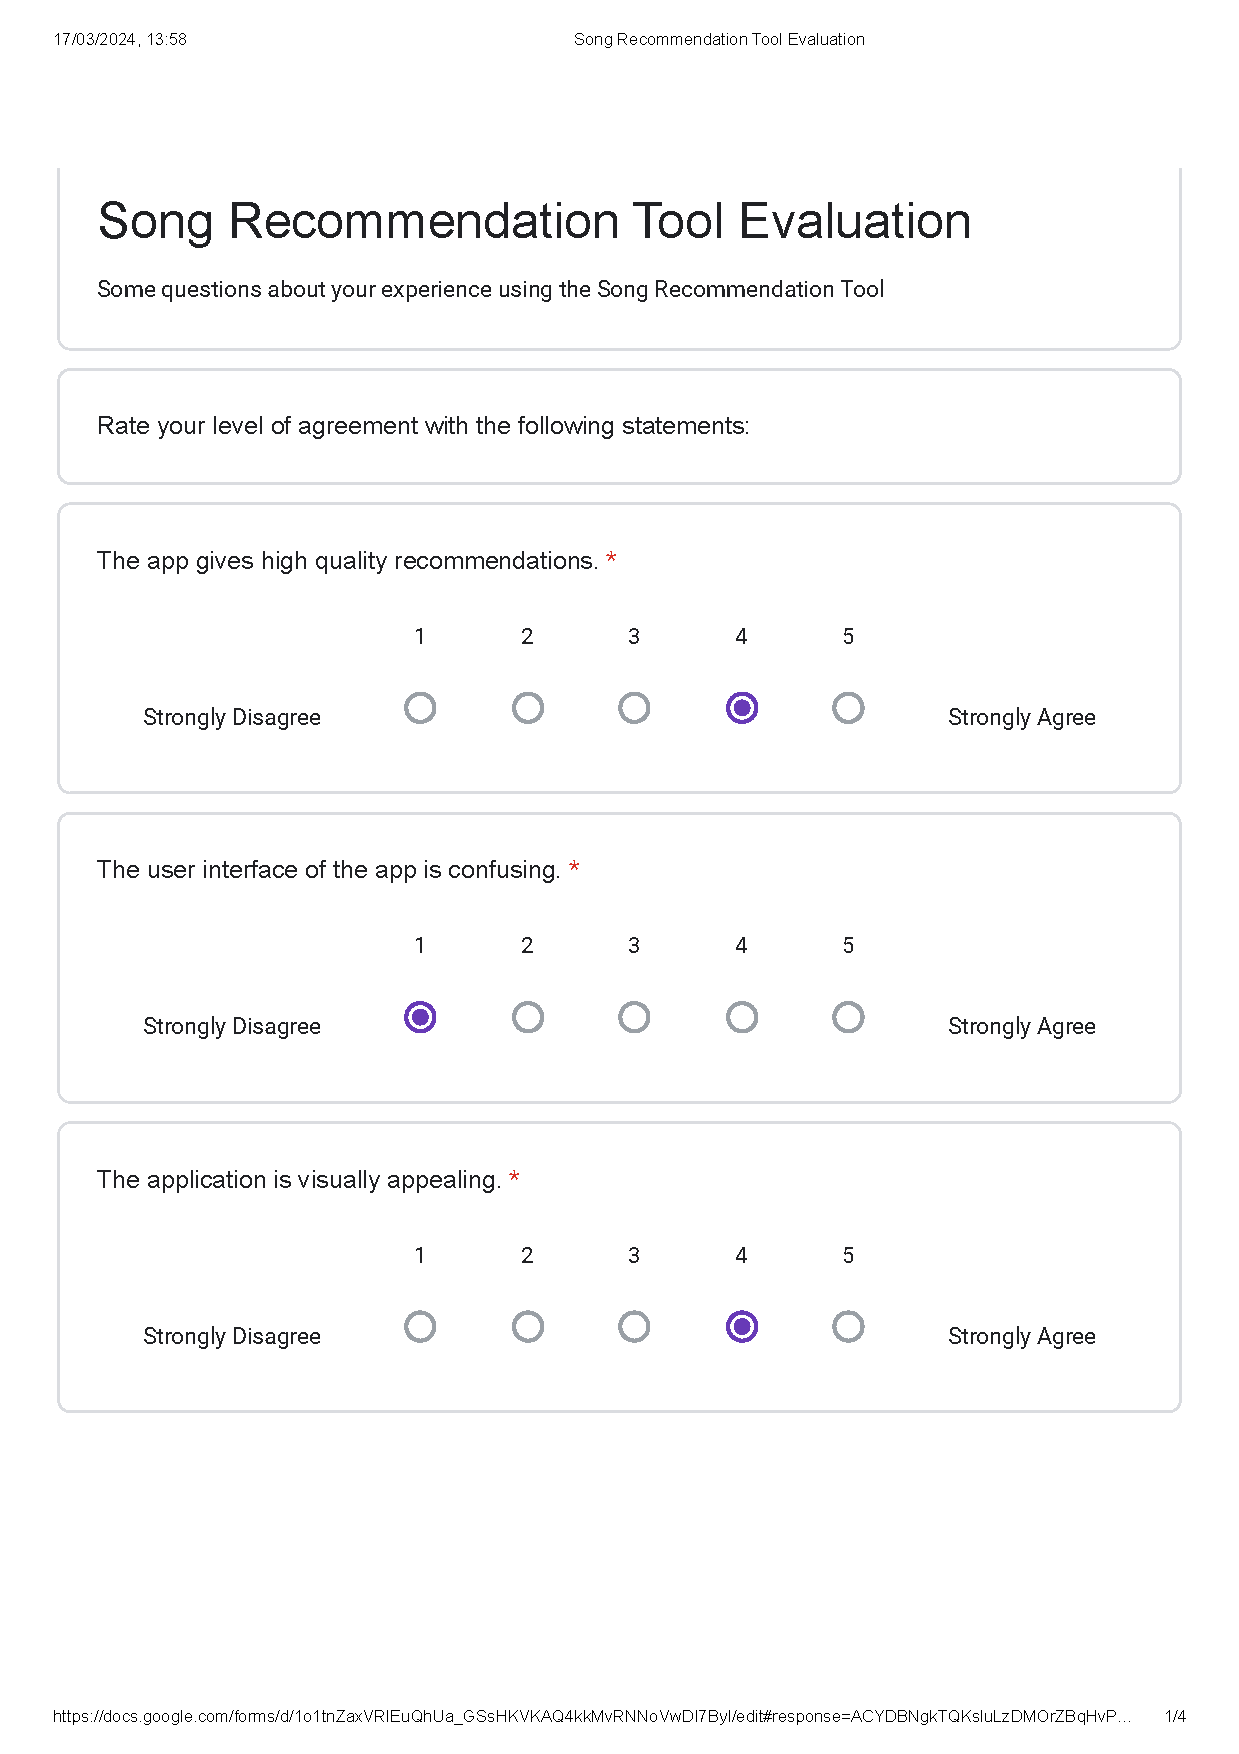
\includepdf[page={1,2,3,4}]{appendices/Song Recommendation Tool Evaluation - Google Forms - 2}
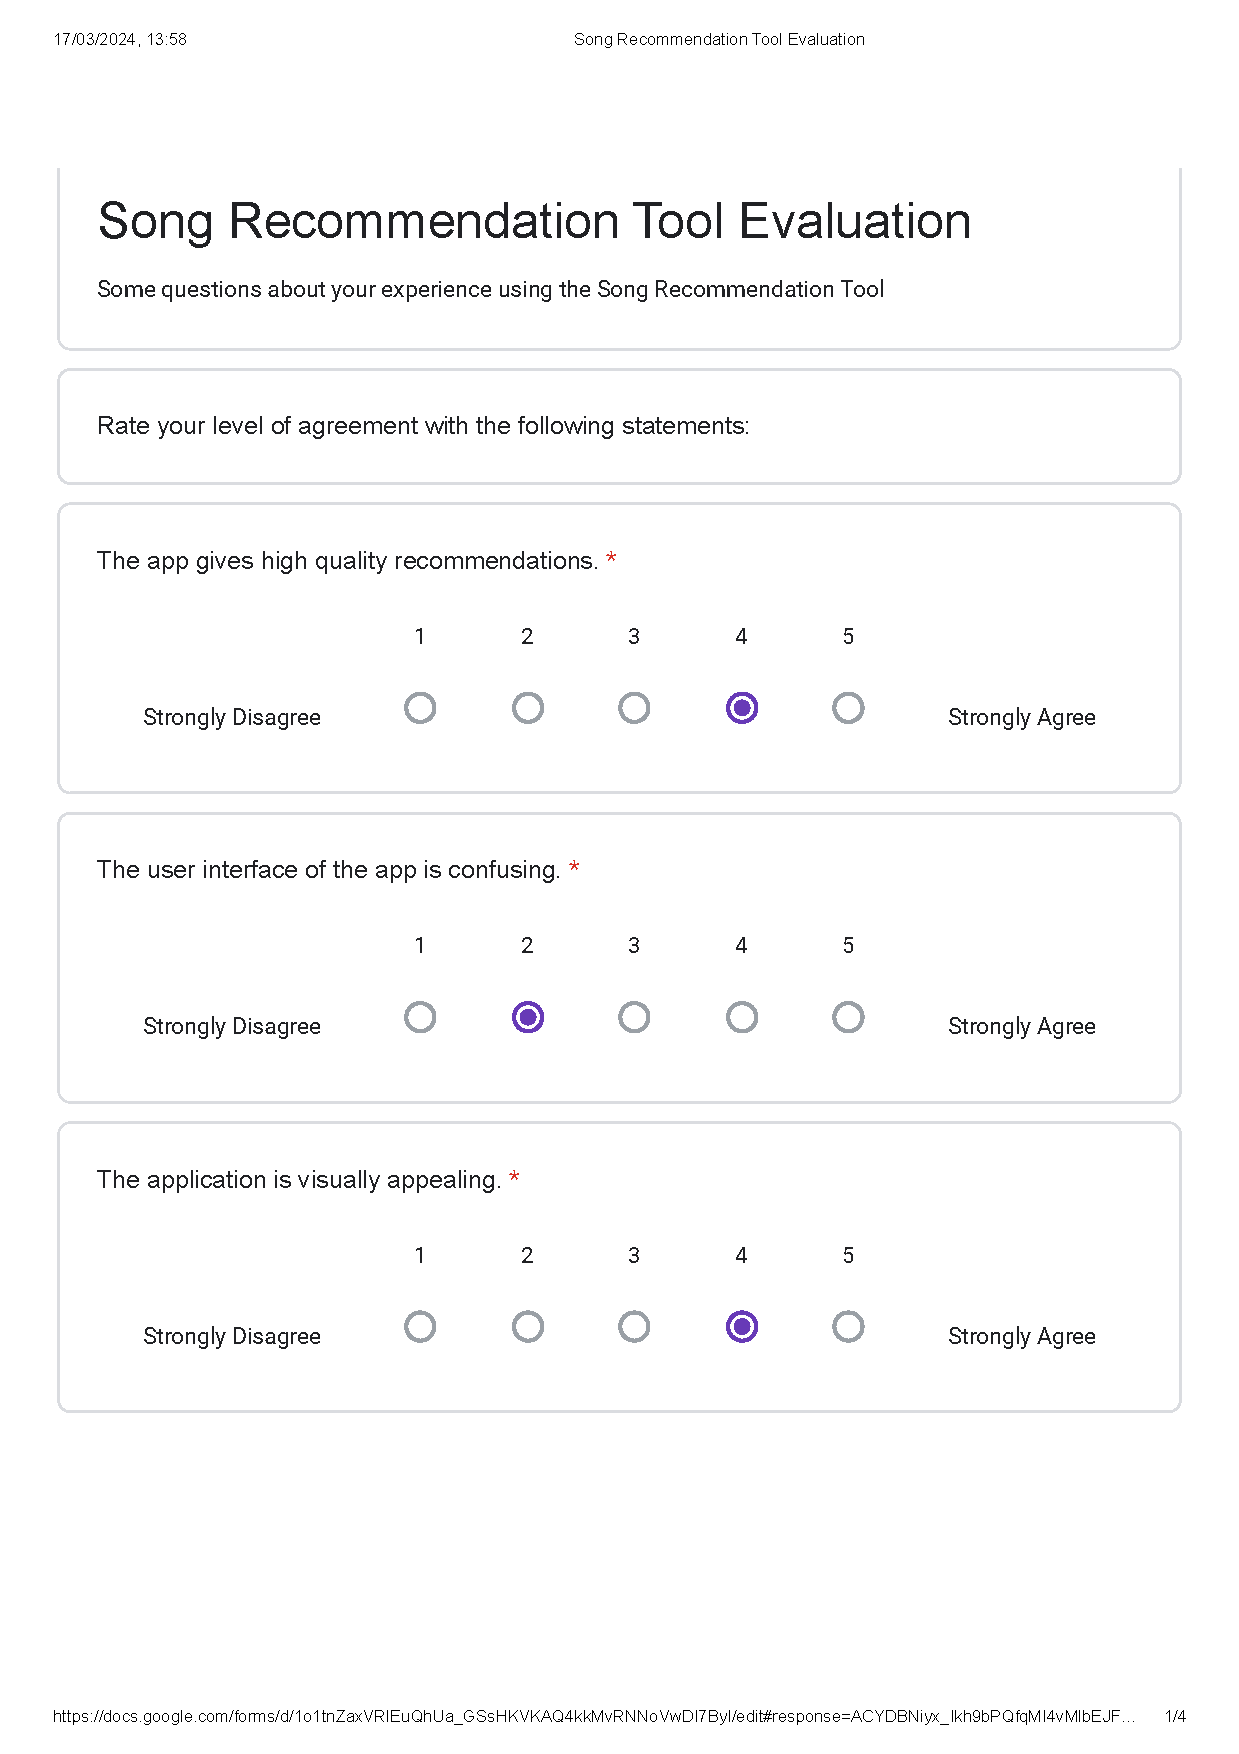
\includepdf[page={1,2,3,4}]{appendices/Song Recommendation Tool Evaluation - Google Forms - 3}
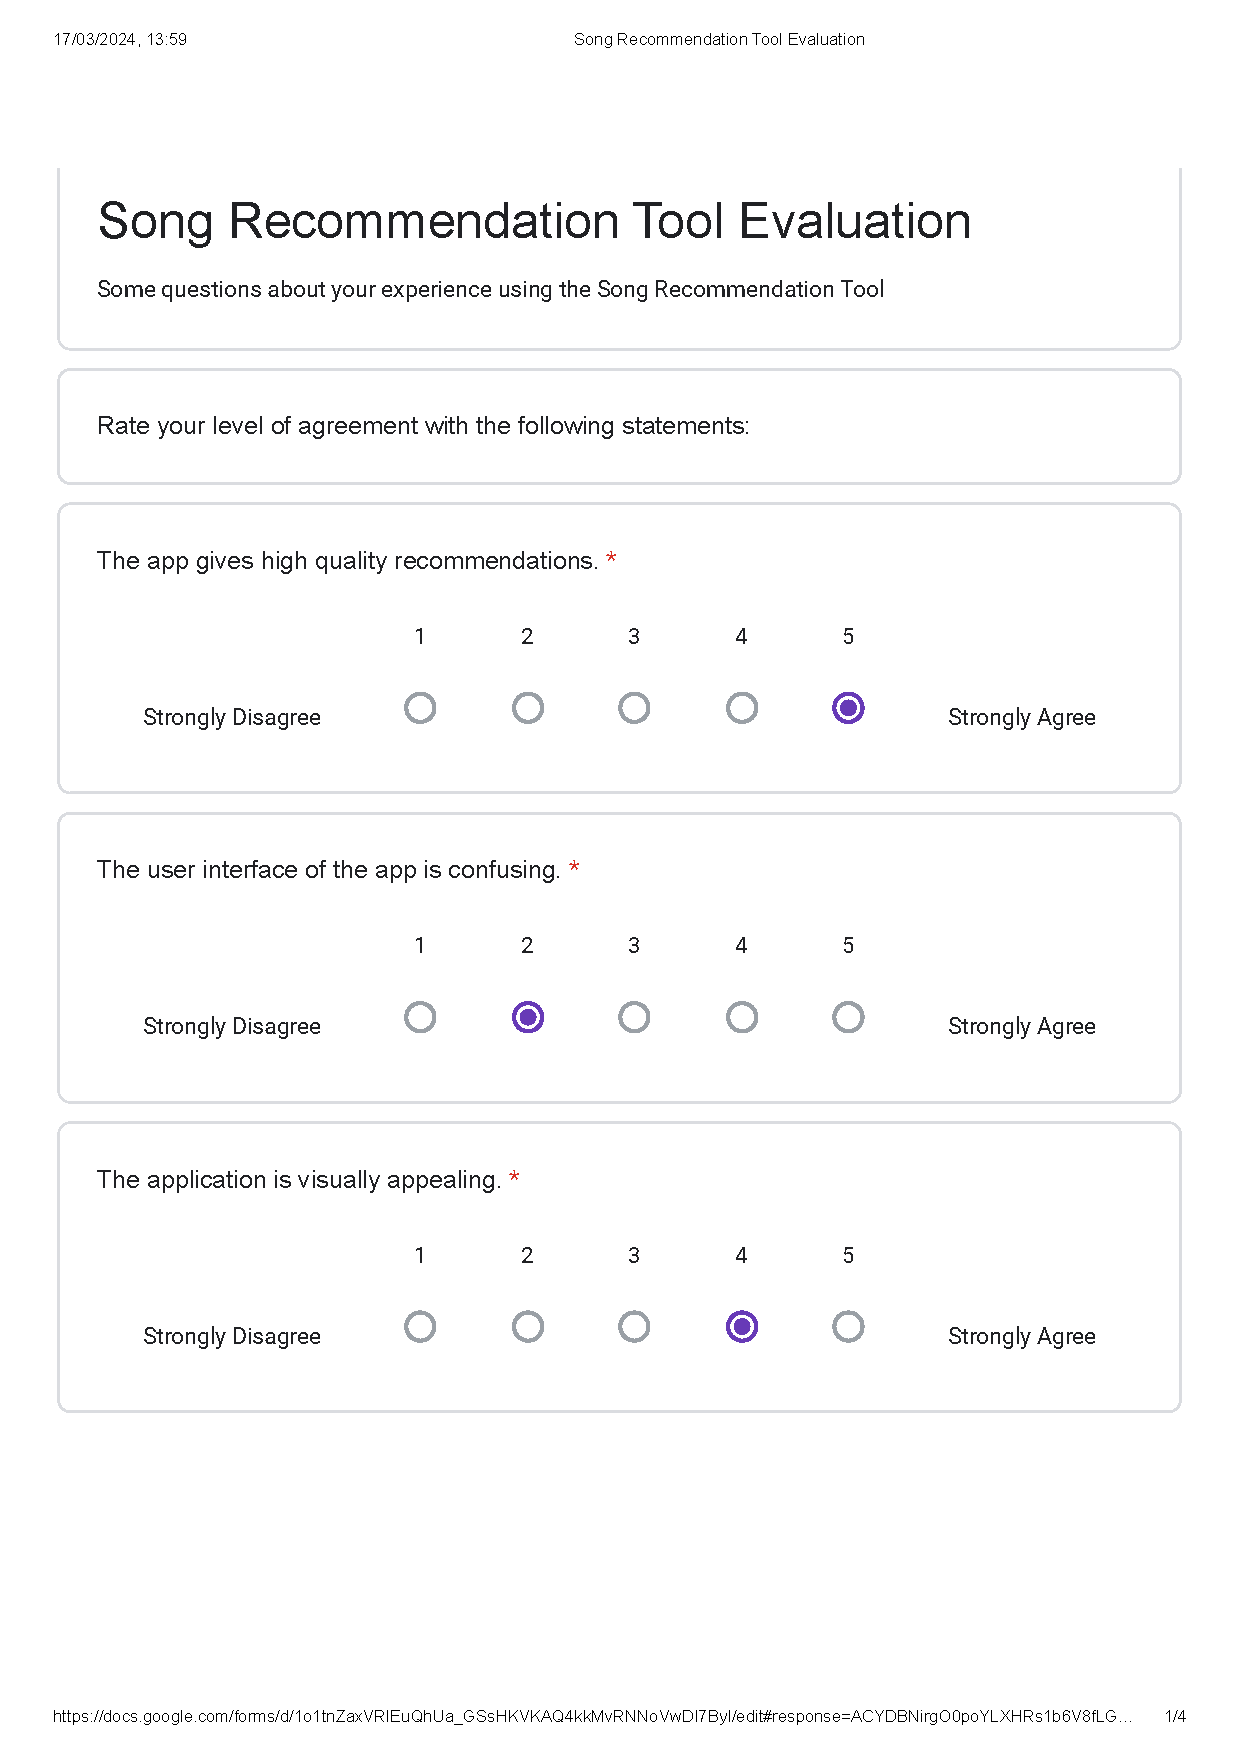
\includepdf[page={1,2,3,4}]{appendices/Song Recommendation Tool Evaluation - Google Forms - 4}
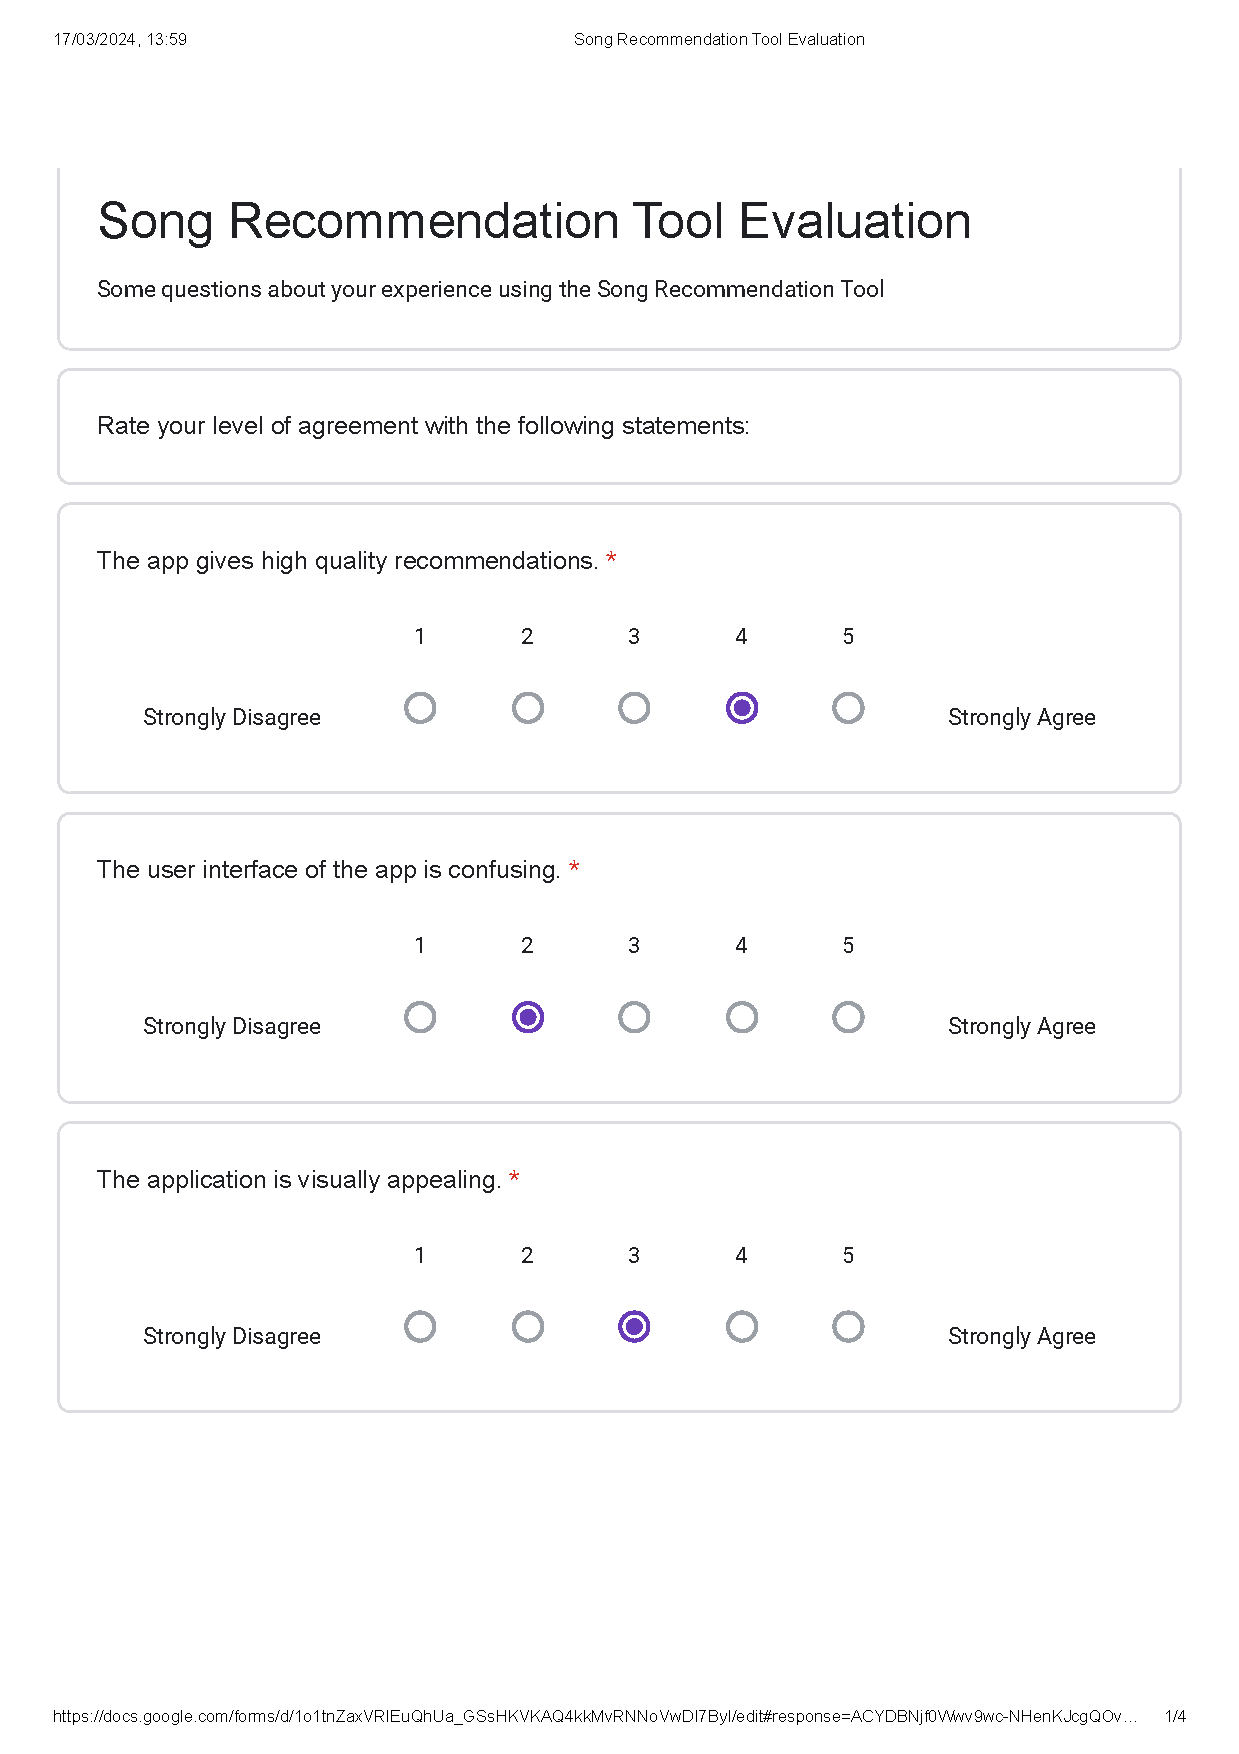
\includepdf[page={1,2,3,4}]{appendices/Song Recommendation Tool Evaluation - Google Forms - 5}
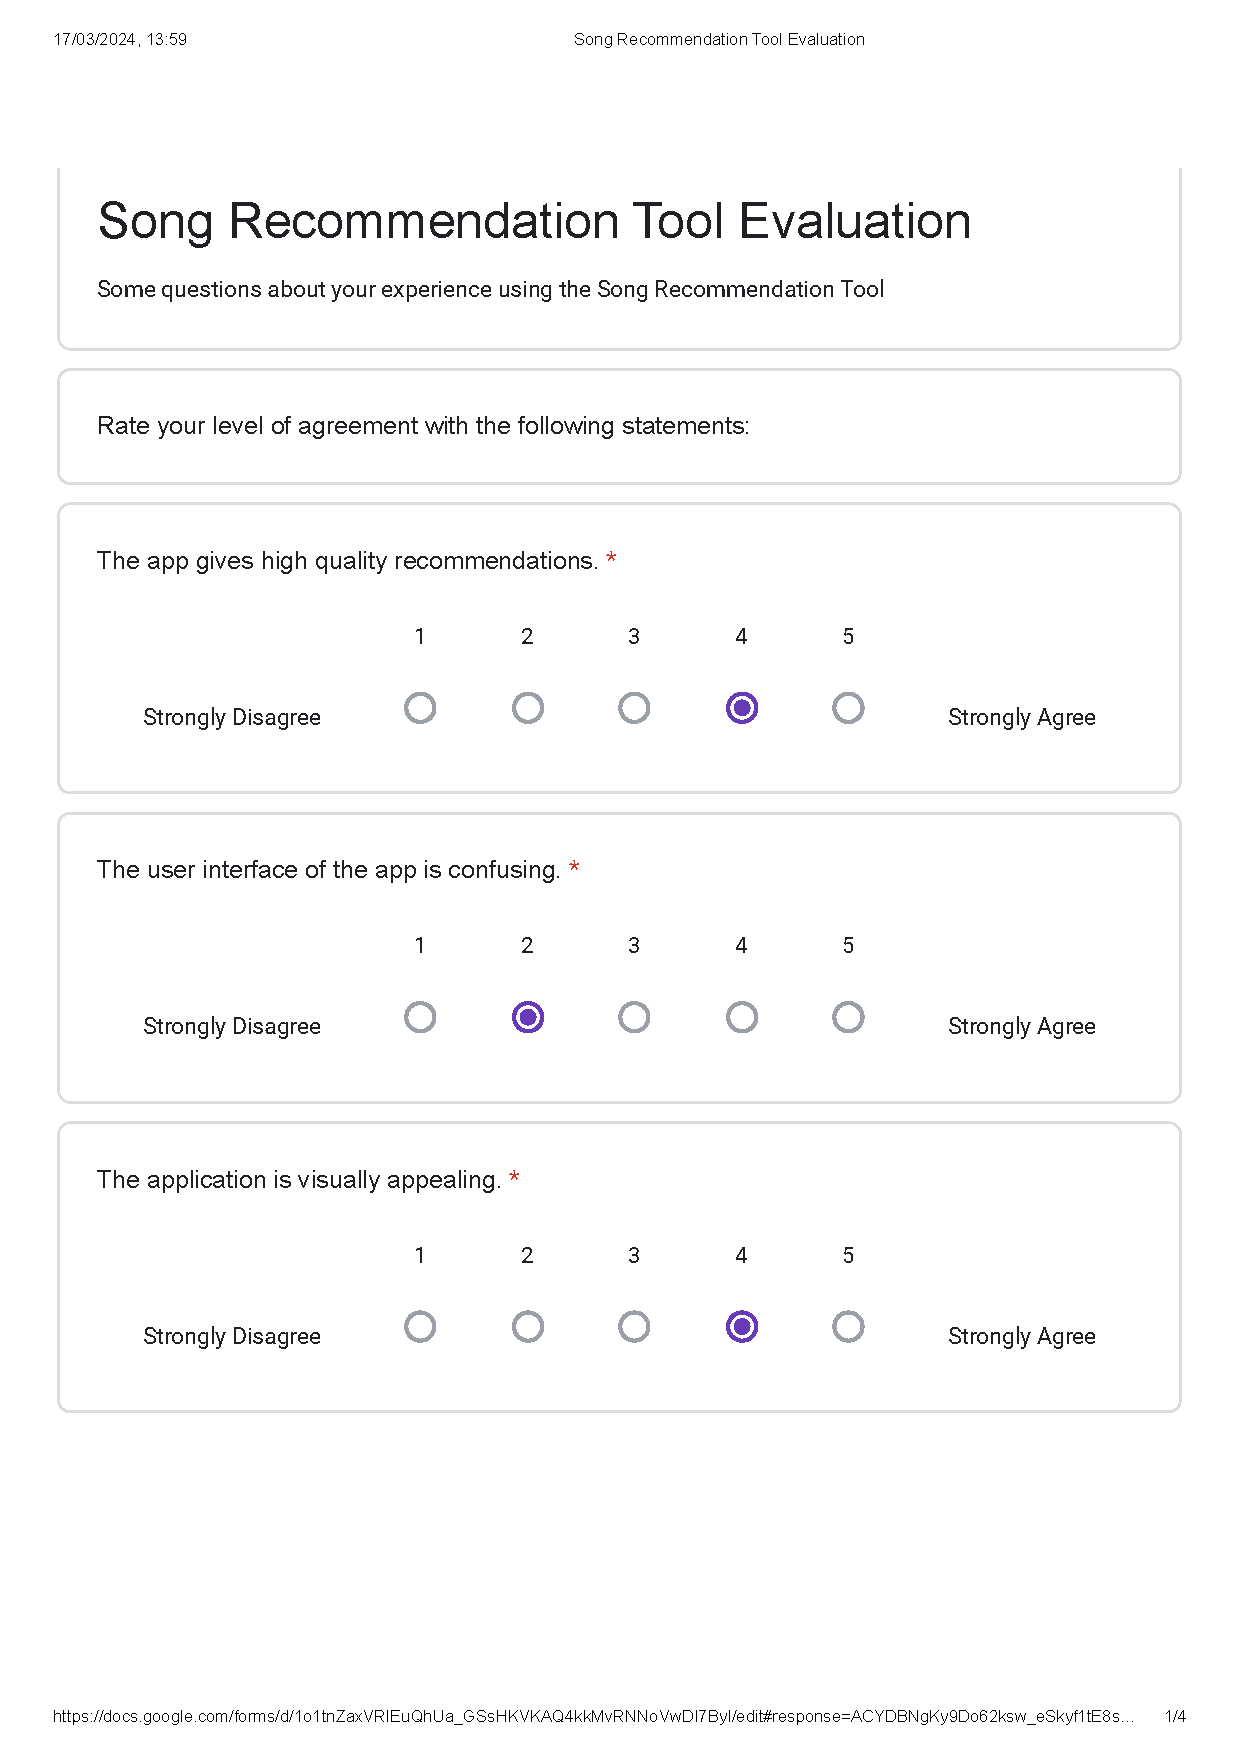
\includepdf[page={1,2,3,4}]{appendices/Song Recommendation Tool Evaluation - Google Forms - 6}
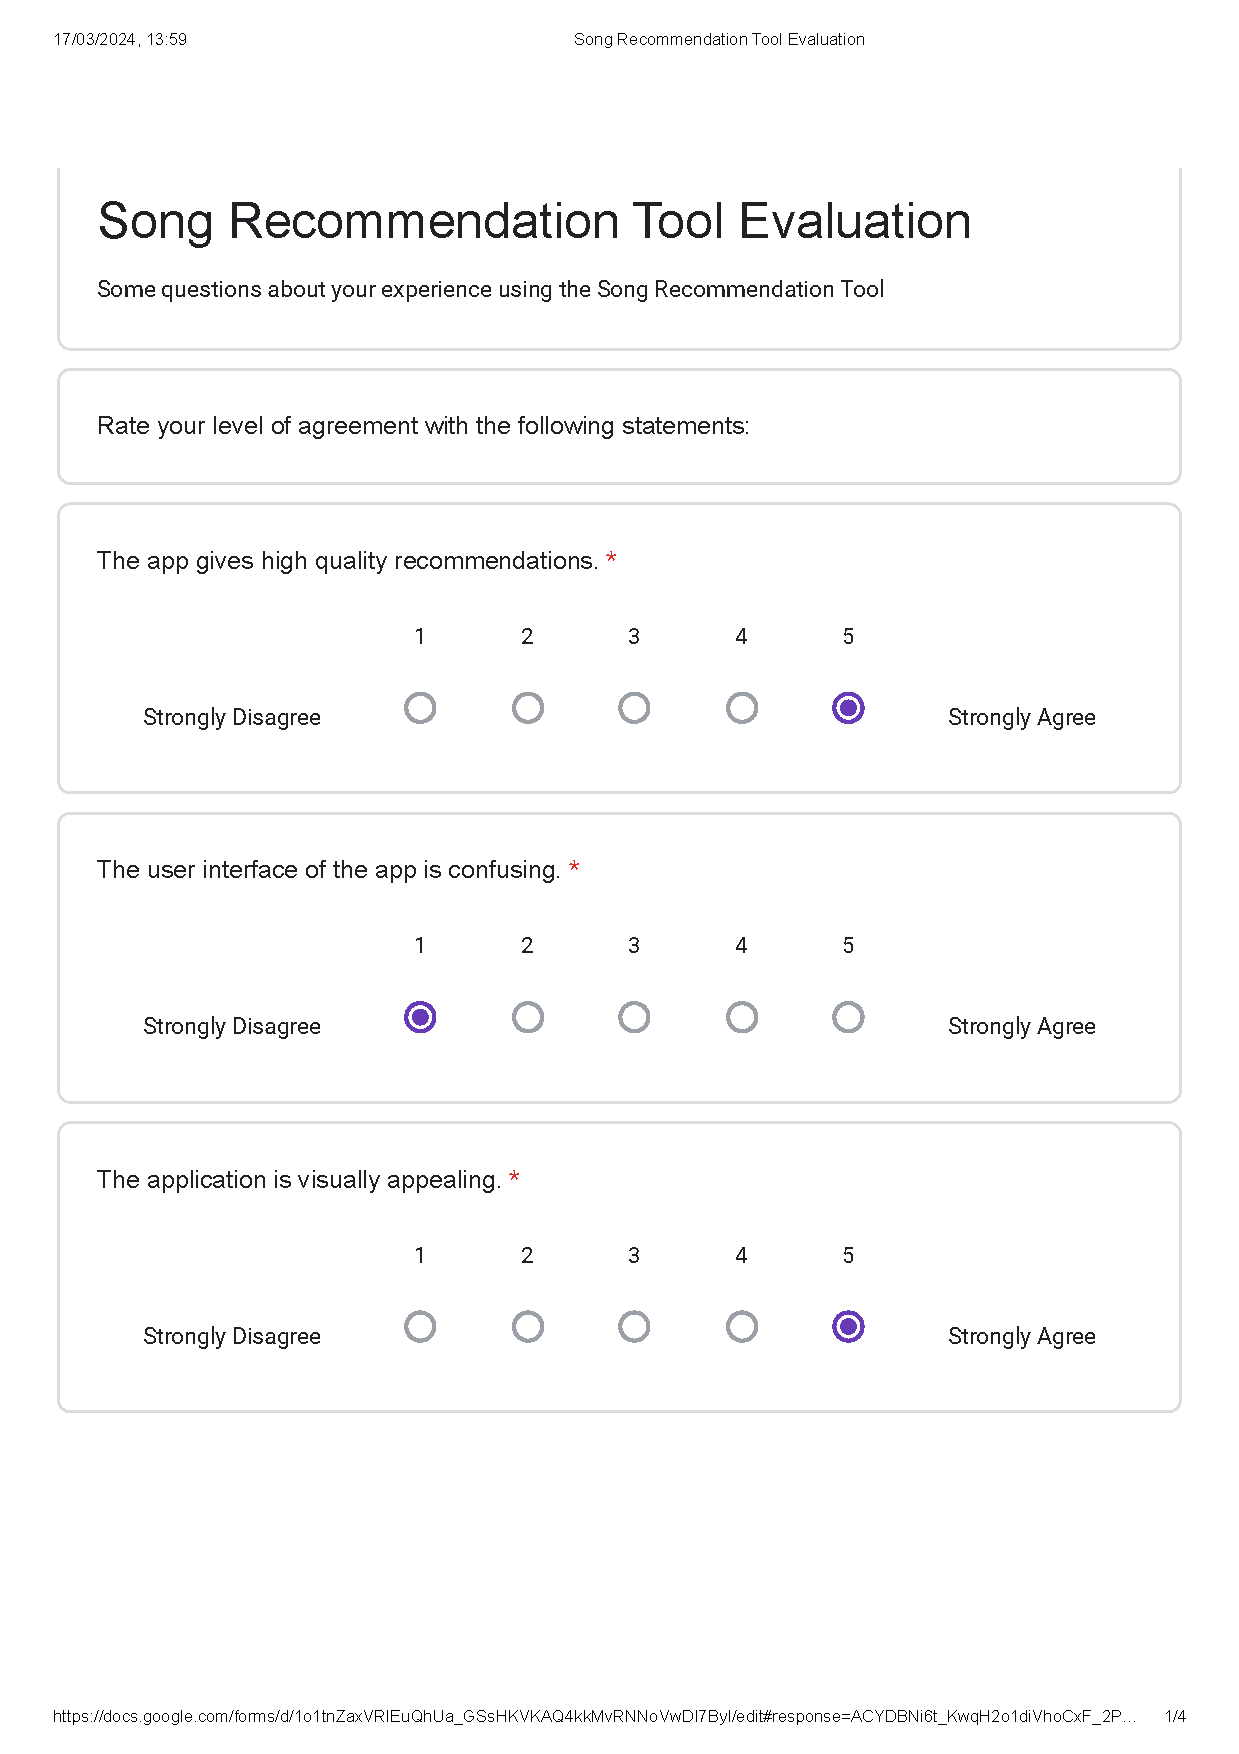
\includepdf[page={1,2,3,4}]{appendices/Song Recommendation Tool Evaluation - Google Forms - 7}
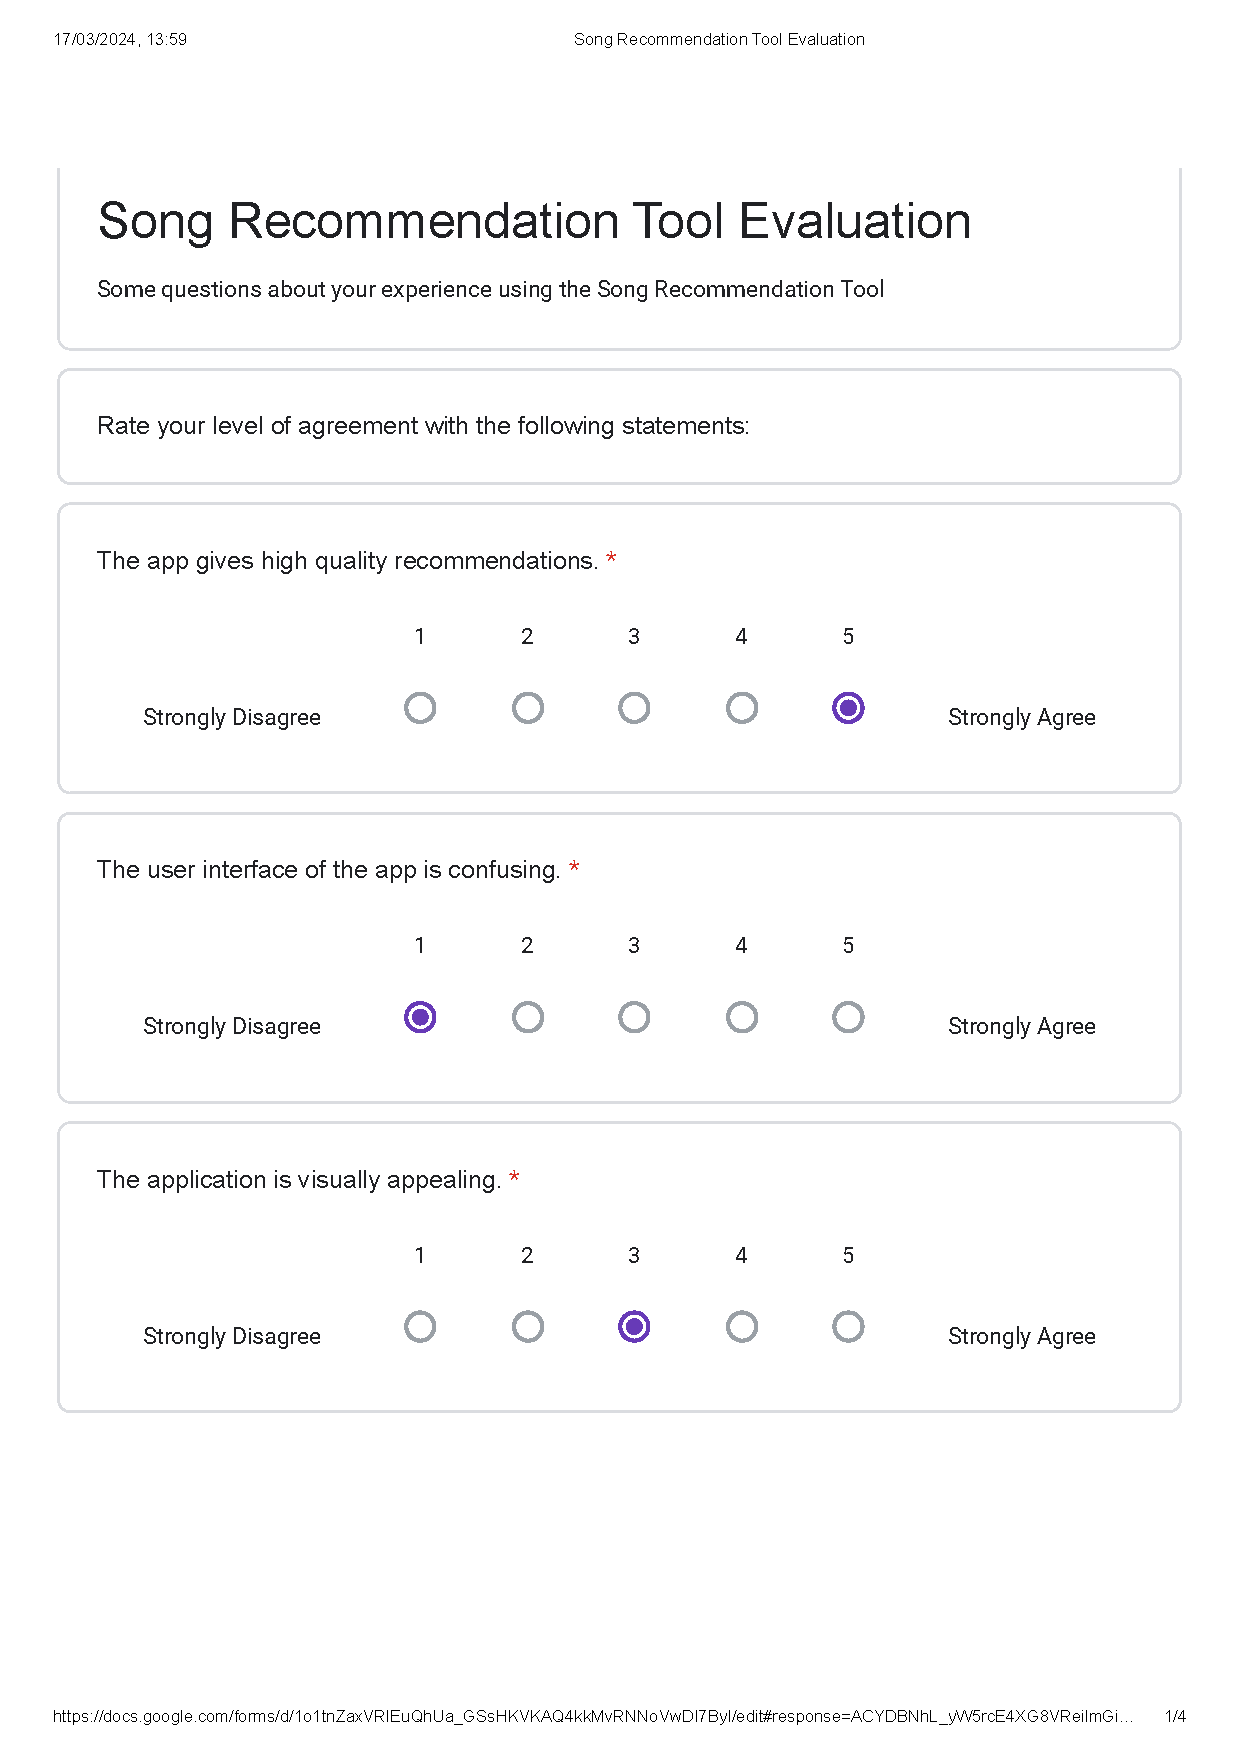
\includepdf[page={1,2,3,4}]{appendices/Song Recommendation Tool Evaluation - Google Forms - 8}
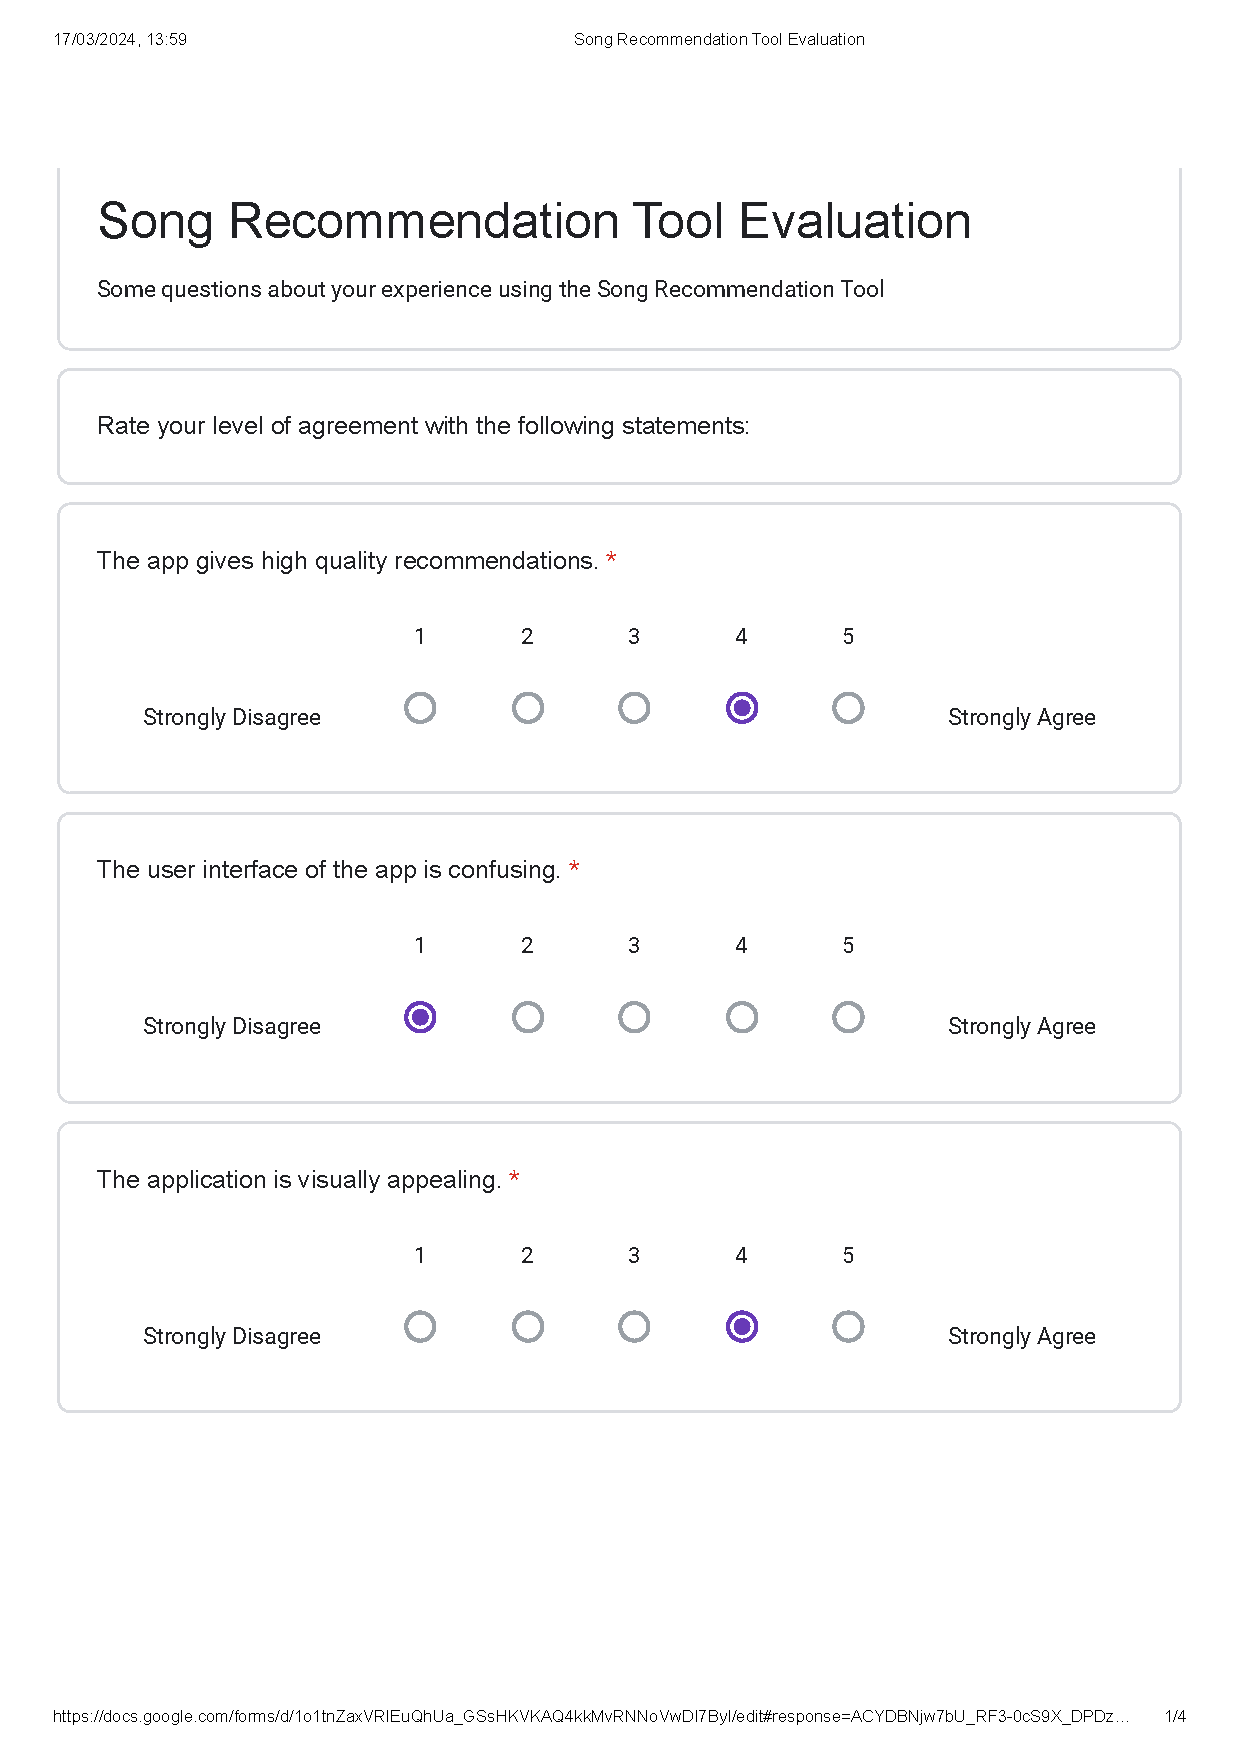
\includepdf[page={1,2,3,4}]{appendices/Song Recommendation Tool Evaluation - Google Forms - 9}
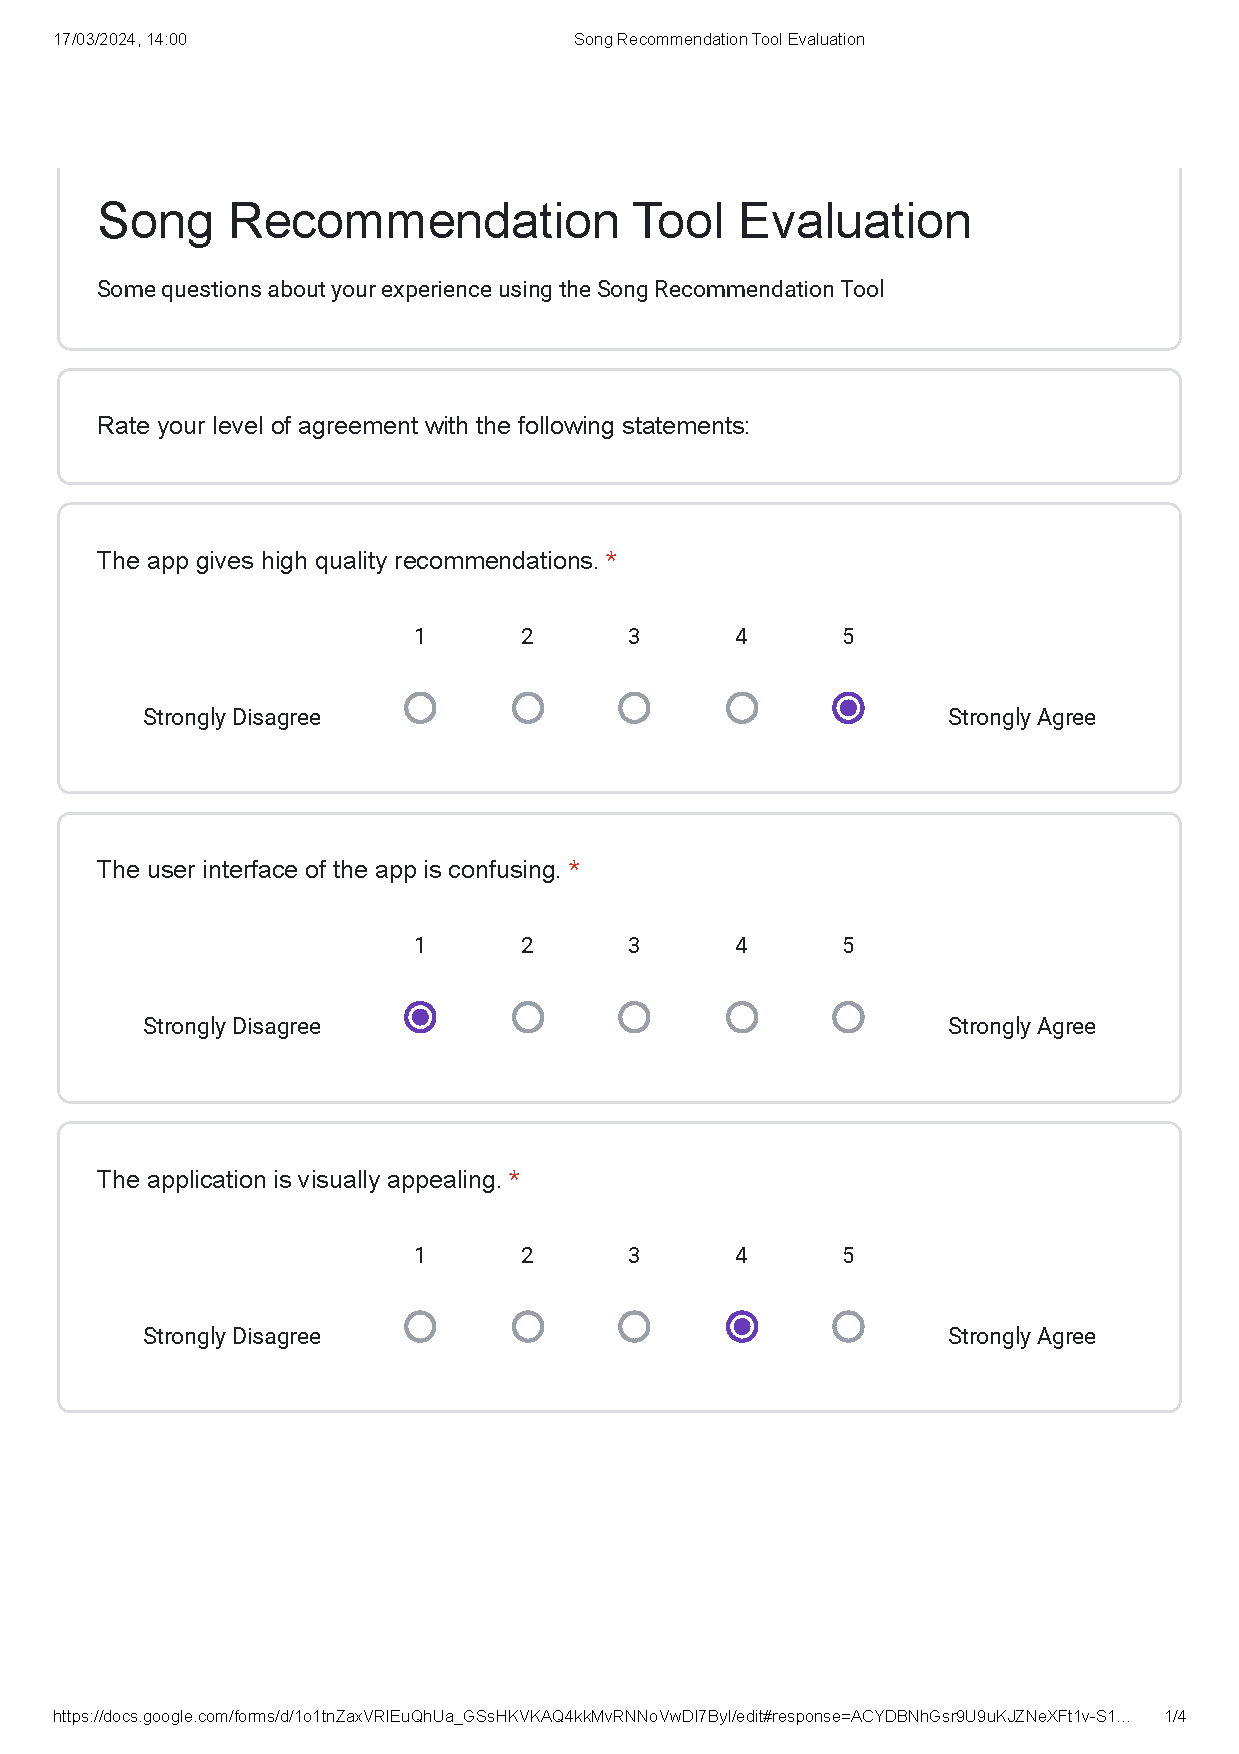
\includepdf[page={1,2,3,4}]{appendices/Song Recommendation Tool Evaluation - Google Forms - 10}

\chapter{User Manual}
On next page.
\begin{figure}
    \centering
    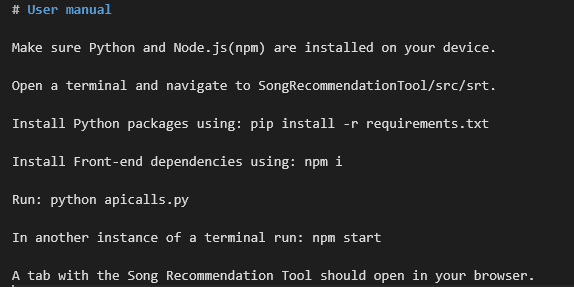
\includegraphics[width=1\linewidth]{appendices/image_2024-03-17_142801856.png}
    \caption{User Manual}
    \label{fig:enter-label}
\end{figure}

\chapter{Project Directory Structure}
On next page.
\includepdf[page={1,2}]{appendices/Song Recommendation Tooldir}

\end{appendices}


%==================================================================================================================================
%   BIBLIOGRAPHY   

% The bibliography style is abbrvnat
% The bibliography always appears last, after the appendices.

\bibliographystyle{abbrvnat}

\bibliography{l4proj.bib}

\end{document}
